\section{Predicting House Sale Prices with Statistical Modeling and
Neural
Networks}\label{predicting-house-sale-prices-with-statistical-modeling-and-neural-networks}

\textbf{Project Report}

\begin{itemize}
\tightlist
\item
  \textbf{Student 1:} Gayakpa Kenny --- 22510580
\item
  \textbf{Student 2:} Khaireddine Gatti
\end{itemize}

\emph{Computational Statistics --- Spring 2026 --- May 27, 2026}

\subsection{Abstract}\label{abstract}

This report presents a statistical and machine-learning analysis of the
Kaggle \emph{House Prices --- Advanced Regression Techniques} dataset,
which describes 1460 residential homes in Ames, Iowa through 79
explanatory variables. The work is organised in five complementary
parts, applied in parallel on three target scales (\texttt{SalePrice},
\texttt{SalePrice\_Log}, \texttt{SalePrice\_BoxCox}) to assess the
robustness of every conclusion across transformations.

We first characterise the distribution of \texttt{SalePrice} through
classical inference (descriptive statistics, 95\% confidence intervals,
one-sample t-tests against \$180,000, Shapiro--Wilk normality tests),
confirming the strong right-skew that motivates the \texttt{log1p} and
Box--Cox transformations. We then identify the ordinal features that
significantly influence price via one-way ANOVA, and quantify pairwise
interactions through a two-way ANOVA assisted by Tukey HSD post-hoc
tests and a structural level-merging strategy. A 2³ factorial design on
three dominant factors decomposes the price structure into main effects
and interactions. A linear regression model (OLS, with Ridge and Lasso
comparisons) built on the significant features supplemented by
\texttt{GrLivArea} and \texttt{TotalBsmtSF} reaches R² ≈ 0.82. Finally,
a multi-layer perceptron trained on all 79 features and tuned via 3-fold
cross-validated grid search achieves a CV RMSE of 0.1821 on the log
scale and a Kaggle public leaderboard RMSE of 0.15591, surpassing both
the OLS benchmark and the CV estimate. The convergence of feature
rankings across parametric and non-parametric methods
(\texttt{GrLivArea}, \texttt{OverallQual}, and \texttt{KitchenQual}
dominate every method) confirms the robustness of the structural
conclusions, while the modest gain of the MLP over OLS indicates that
the bulk of the predictive signal is already captured by a small number
of dominant features.

\begin{center}\rule{0.5\linewidth}{0.5pt}\end{center}

\subsection{Contents}\label{contents}

\begin{enumerate}
\def\labelenumi{\arabic{enumi}.}
\tightlist
\item
  \hyperref[1-introduction]{Introduction}
\item
  \hyperref[2-data-and-preprocessing]{Data and Preprocessing}
\item
  \hyperref[3-classical-statistical-inference]{Classical Statistical
  Inference}
\item
  \hyperref[4-anova-for-ordinal-features]{ANOVA for Ordinal Features}
\item
  \hyperref[5-2k-factorial-design]{2\^{}k Factorial Design}
\item
  \hyperref[6-parametric-regression]{Parametric Regression}
\item
  \hyperref[7-neural-network-regression]{Neural-Network Regression}
\item
  \hyperref[8-conclusion]{Conclusion}
\item
  \hyperref[individual-contributions]{Individual Contributions}
\end{enumerate}

\begin{center}\rule{0.5\linewidth}{0.5pt}\end{center}

\subsection{1 Introduction}\label{introduction}

\subsubsection{What the project is
about}\label{what-the-project-is-about}

This project tackles a classic problem in applied statistical learning:
predicting the sale price of residential houses. The work is built on
the \emph{House Prices --- Advanced Regression Techniques} dataset
hosted on Kaggle, which describes the residential real estate. The
objective is twofold: first, to understand which factors genuinely drive
the price of a house through a thorough statistical analysis; second, to
build a predictive model capable of generalising to unseen houses, whose
predictions are submitted to Kaggle and evaluated through the RMSE.

More broadly, the project serves as a framework for applying a coherent
set of statistical and machine-learning techniques: classical inference,
analysis of variance, factorial experimental design, parametric
regression, and a non-parametric neural network model. Each method
answers a distinct question about the data, and their progressive
articulation forms the backbone of the project.

\subsubsection{Outline of the project}\label{outline-of-the-project}

The work is organised into five parts.

\textbf{Part 1 --- Classical statistical inference.} We begin by
characterising the distribution of \texttt{SalePrice} (mean, variance,
95\% confidence interval), then formally test several hypotheses: does
the mean differ from \$180,000? Is the distribution normal
(Shapiro--Wilk test)? This part also introduces the two transformations
(\texttt{log1p} and Box--Cox) that will serve as alternative targets
throughout the rest of the project.

\textbf{Part 2 --- ANOVA and identification of significant features.}
Out of ten candidate variables, we identify via a one-way ANOVA those
that have a statistically significant effect on price. We then proceed
with a two-way ANOVA to detect interactions between pairs of variables,
relying on Tukey HSD post-hoc tests and a level-merging strategy.

\textbf{Part 3 --- 2³ Factorial Design.} We binarise three of the
significant factors to build a 2³ experimental design. This compact
structure allows the price to be decomposed into main effects, two-way
interactions, and the three-way interaction, and to visually identify
the couplings between factors through interaction plots.

\textbf{Part 4 --- Parametric regression.} We build a linear regression
model (OLS) using the significant ordinal features, supplemented by two
numerical variables (\texttt{GrLivArea}, \texttt{TotalBsmtSF}). The
analysis covers the coefficients, their p-values, residual diagnostics,
and a comparison with the regularised Ridge and Lasso variants.

\textbf{Part 5 --- Non-parametric model (neural network).} The final
part leverages all 79 available variables to train a multi-layer
perceptron (MLP). We build a complete preprocessing pipeline
(imputation, one-hot encoding, standardisation), tune the
hyperparameters via \texttt{GridSearchCV}, analyse the residuals of the
final model, and generate the \texttt{submission.csv} file submitted to
Kaggle.

Three scales of the target (\texttt{SalePrice}, \texttt{SalePrice\_Log},
\texttt{SalePrice\_BoxCox}) are kept in parallel across Parts 1 to 4,
allowing every step to compare the robustness of conclusions across
transformations.

\begin{center}\rule{0.5\linewidth}{0.5pt}\end{center}

\subsection{2 Data and Preprocessing}\label{data-and-preprocessing}

\subsubsection{2.1 Data Source}\label{data-source}

The dataset used in this project is the \emph{House Prices --- Advanced
Regression Techniques} corpus, hosted by Kaggle {[}2{]}. The data is
delivered in two CSV files:

\begin{itemize}
\tightlist
\item
  \textbf{\texttt{train.csv}} --- 1460 houses, each accompanied by 81
  columns: a unique identifier \texttt{Id}, the target variable
  \texttt{SalePrice} (the actual sale price in US dollars), and 79
  explanatory variables.
\item
  \textbf{\texttt{test.csv}} --- 1459 houses described by the same 79
  explanatory variables, but without the \texttt{SalePrice} column.
  These are the houses for which a prediction must be produced.
\end{itemize}

The split between training and test sets is fixed by Kaggle and cannot
be modified --- the test set is the official evaluation set against
which submissions are scored. The evaluation metric is the Root Mean
Squared Error (RMSE) computed on the logarithm of the predicted price.

The 79 explanatory variables describe (almost) every aspect of
residential homes. Of these, \textbf{36 are numerical} (\texttt{int64},
\texttt{float64}) and \textbf{43 are categorical} (\texttt{object}). The
categorical variables are predominantly ordinal quality scales (e.g.,
\texttt{Po}, \texttt{Fa}, \texttt{TA}, \texttt{Gd}, \texttt{Ex}), with
some nominal attributes such as \texttt{Neighborhood} (25 distinct
levels --- the highest cardinality of the dataset). Numerical variables
include surfaces (\texttt{GrLivArea}, \texttt{TotalBsmtSF},
\texttt{LotArea}), counts, and years.

\subsubsection{2.2 Preprocessing
Decisions}\label{preprocessing-decisions}

\paragraph{Handling the target
variable}\label{handling-the-target-variable}

The variable \texttt{SalePrice} is heavily right-skewed (skewness =
1.883). Since most statistical methods used in this project (t-tests,
ANOVA, OLS regression) and the Kaggle evaluation metric itself assume
approximate symmetry on the target, a transformation that brings the
distribution closer to a bell curve is needed. Two candidates are
evaluated and kept in parallel throughout Parts 1 to 4.

\begin{figure}
\centering
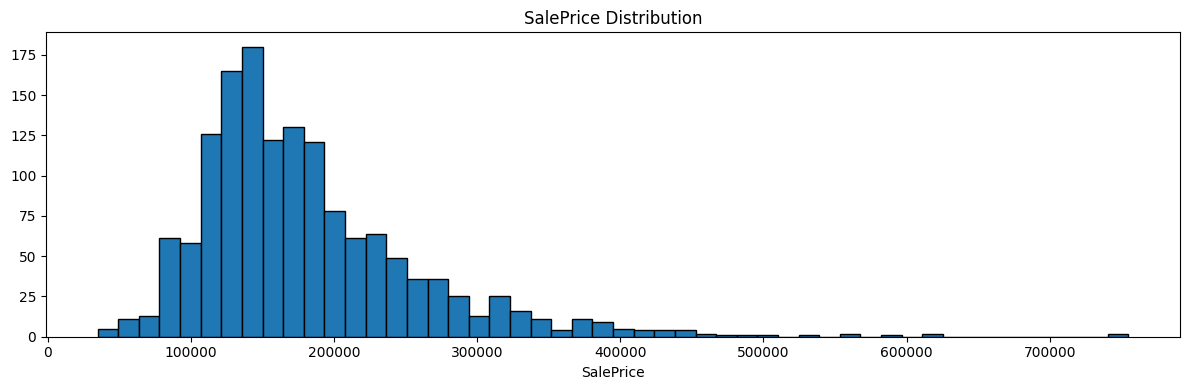
\includegraphics{figures/saleprice_distribution.png}
\caption{Distribution of SalePrice on the training set}
\end{figure}

\emph{Figure 1: Distribution of \texttt{SalePrice} on the training set.
The histogram shows the strong right-skew (skewness = 1.883) that
motivates the use of the \texttt{log1p} and Box--Cox transformations.}

\textbf{The logarithmic transformation (\texttt{log1p}).} The logarithm
compresses large numbers much more aggressively than small ones, which
is exactly what a right-skewed distribution needs.

\begin{itemize}
\tightlist
\item
  \textbf{Formula:} \(y = \ln(1 + x)\)
\item
  \textbf{Why \texttt{log1p} instead of \texttt{log}:} the +1 shift
  avoids the singularity of \(\ln(0)\), since the natural logarithm is
  undefined at zero.
\item
  \textbf{Effect:} very high prices (the right tail) are pulled toward
  the centre of the distribution, producing a roughly symmetrical bell
  curve.
\end{itemize}

To recover dollar amounts from a log-transformed prediction, we invert
the operation using the exponential function:

\begin{itemize}
\tightlist
\item
  \textbf{Inverse formula:} \(x = e^y - 1\)
\item
  \textbf{In Python:} \texttt{np.expm1(log\_value)}
\end{itemize}

\textbf{The Box--Cox transformation.} Unlike the logarithm, Box--Cox
does not rely on a single fixed formula. Instead, it searches for the
power \(\lambda\) that makes the transformed data as normal as possible.

\begin{itemize}
\tightlist
\item
  \textbf{Formula:}
\end{itemize}

\[y = \begin{cases} \dfrac{x^\lambda - 1}{\lambda} & \text{if } \lambda \neq 0 \\ \ln(x) & \text{if } \lambda = 0 \end{cases}\]

\begin{itemize}
\tightlist
\item
  \textbf{Logic:} the algorithm tests many candidate values of
  \(\lambda\) and retains the one that brings the transformed data
  closest to a normal distribution.
\end{itemize}

The inverse transformation is:

\begin{itemize}
\tightlist
\item
  \textbf{Inverse formula:} \(x = (y \cdot \lambda + 1)^{1/\lambda}\)
\item
  \textbf{In Python:}
  \texttt{scipy.special.inv\_boxcox(bc\_value,\ lmbda)}
\end{itemize}

\textbf{How the algorithm finds the optimal λ.} The procedure proceeds
in three logical steps:

\begin{enumerate}
\def\labelenumi{\arabic{enumi}.}
\tightlist
\item
  \textbf{The ``best score'' test (likelihood).} For each candidate
  value of \(\lambda\), the algorithm computes a score on the
  transformed data. The closer the transformed distribution is to a
  normal one, the higher the score.
\item
  \textbf{Searching for the peak.} The algorithm adjusts \(\lambda\)
  incrementally until it locates the value that produces the highest
  possible score.
\item
  \textbf{Two validation objectives.} A correct \(\lambda\) should
  produce a distribution that satisfies two properties simultaneously:
  \textbf{symmetry} (skewness close to 0) and \textbf{balance} (a
  reduced gap between small and large values).
\end{enumerate}

On our \texttt{SalePrice} data, the search yields
\(\lambda \approx -0.0769\). A \(\lambda\) of exactly 0 would be
equivalent to a pure logarithm, so a \(\lambda\) of \(-0.0769\) means
the data needed a transformation only slightly stronger than
\texttt{log1p} to reach near-perfect symmetry.

\textbf{Comparative demonstration.} The table below shows how both
methods transform a representative sample of price levels. Both compress
the gap between cheap and expensive houses, but Box--Cox (with
\(\lambda = -0.0769\)) is slightly more aggressive on the high end. The
rightmost column confirms that the inverse transformation recovers the
original price exactly in both cases.

\begin{longtable}[]{@{}lllll@{}}
\toprule\noalign{}
House Type & Original Price (x) & y\_log & y\_bc & Return Accuracy \\
\midrule\noalign{}
\endhead
\bottomrule\noalign{}
\endlastfoot
Entry-level & \$50,000 & 10.8198 & 7.3342 & \$50,000 \\
Average Price (Target) & \$180,000 & 12.1007 & 7.8672 & \$180,000 \\
High-end & \$350,000 & 12.7657 & 8.1311 & \$350,000 \\
Luxury (Outlier) & \$500,000 & 13.1224 & 8.2444 & \$500,000 \\
Ultra-Luxury & \$750,000 & 13.5278 & 8.4005 & \$750,000 \\
\end{longtable}

\textbf{Detailed calculation example.} Consider a house priced at
exactly \$300,000 and follow each step of the round-trip.

\emph{Case A --- Logarithm (\texttt{log1p}).}

\begin{enumerate}
\def\labelenumi{\arabic{enumi}.}
\tightlist
\item
  \textbf{Transformation:} \(y = \ln(1 + 300{,}000) \approx 12.6115\)
\item
  \textbf{Reverse (return to price):}

  \begin{itemize}
  \tightlist
  \item
    \(x = e^{12.6115} - 1\)
  \item
    \(x = 300{,}001 - 1 = \$300{,}000\)
  \end{itemize}
\end{enumerate}

\emph{Case B --- Box--Cox (with \(\lambda = -0.0769\)).}

\begin{enumerate}
\def\labelenumi{\arabic{enumi}.}
\tightlist
\item
  \textbf{Transformation:}

  \begin{itemize}
  \tightlist
  \item
    \(y = \dfrac{300{,}000^{-0.0769} - 1}{-0.0769}\)
  \item
    \(300{,}000^{-0.0769} \approx 0.37985\)
  \item
    \(y = \dfrac{0.37985 - 1}{-0.0769} = \dfrac{-0.62015}{-0.0769} \approx 8.0644\)
  \end{itemize}
\item
  \textbf{Reverse (return to price):}

  \begin{itemize}
  \tightlist
  \item
    \(x = (8.0644 \cdot -0.0769 + 1)^{1/-0.0769}\)
  \item
    \(x = (-0.62015 + 1)^{-13.0039}\)
  \item
    \(x = (0.37985)^{-13.0039} \approx \$300{,}000\)
  \end{itemize}
\end{enumerate}

\textbf{Applying the transformations to the data.} Having defined both
transformations theoretically, we now apply them to the
\texttt{SalePrice} column and inspect the result. The code creates the
two new variables \texttt{SalePrice\_Log} and
\texttt{SalePrice\_BoxCox}, computes the skewness on each scale to
verify the effect of each transformation, and produces a three-panel
histogram comparing the original distribution against its two normalised
counterparts.

From this point on, the two transformed variables
\texttt{SalePrice\_Log} and \texttt{SalePrice\_BoxCox} are kept
alongside the original \texttt{SalePrice} as three parallel targets
across Parts 1 to 4. For Part 5 (neural network), only
\texttt{SalePrice\_Log} is used as the training target, because the
Kaggle evaluation metric itself operates on the log scale.

\begin{figure}
\centering
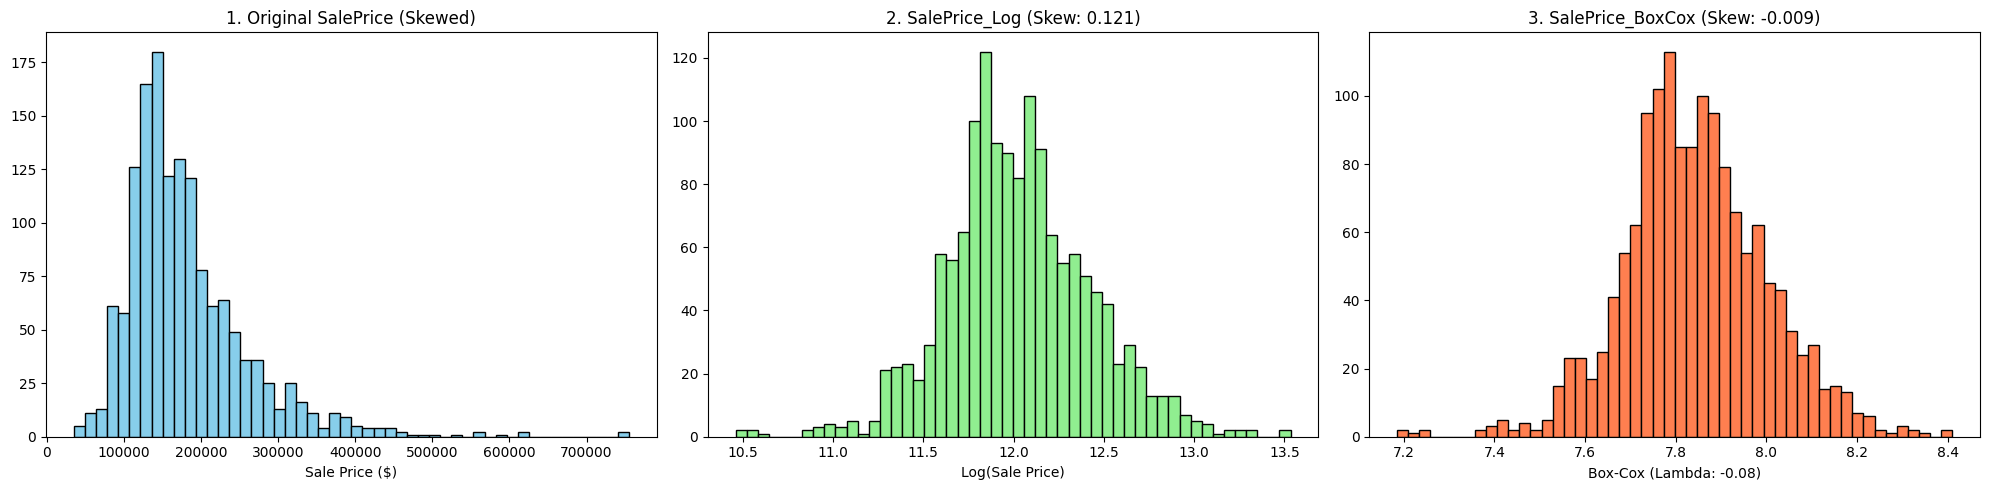
\includegraphics{figures/transformations_comparison.png}
\caption{Visual comparison of three target scales}
\end{figure}

\emph{Figure 2: Visual comparison of the three target scales: original
\texttt{SalePrice} (skewed), \texttt{SalePrice\_Log} (skewness 0.121),
and \texttt{SalePrice\_BoxCox} with \(\lambda = -0.08\) (skewness
\(-0.009\)).}

\paragraph{Interpretation of Skewness and Statistical
Transformations}\label{interpretation-of-skewness-and-statistical-transformations}

\textbf{Statistical rule of symmetry:}

\begin{quote}
\textbf{The Skewness Rule:} A perfectly symmetrical distribution (a
perfect bell curve) has a skewness of 0. - Between \(-0.5\) and \(0.5\):
The data is considered ``fairly symmetrical''. - Greater than 1 or less
than \(-1\): The data is ``highly skewed''.
\end{quote}

\textbf{1. Original SalePrice (Skewness: 1.883).}

\begin{itemize}
\tightlist
\item
  \textbf{The Deduction:} With a score of 1.883, the original data is
  \textbf{highly skewed}.
\item
  \textbf{The Rule:} This exceeds the threshold of 1.0. This ``positive
  skew'' indicates a long tail to the right.
\item
  \textbf{The Impact:} If we use this value as-is, our future models
  will make large errors on average-priced houses.
\end{itemize}

\textbf{2. After Log Transformation (Skewness: 0.121).}

\begin{itemize}
\tightlist
\item
  \textbf{The Deduction:} By applying the Log, we brought the skewness
  down from 1.883 to 0.121.
\item
  \textbf{The Rule:} Since 0.121 is between \(-0.5\) and \(0.5\), the
  data is now considered \textbf{fairly symmetrical}.
\end{itemize}

\textbf{3. After Box-Cox Transformation (Skewness: \(-0.009\)).}

\begin{itemize}
\tightlist
\item
  \textbf{The Deduction:} Box-Cox is the winner with a score of
  \(-0.009\), which is almost absolute zero.
\item
  \textbf{The Rule of Lambda (\(\lambda\)):} Box-Cox Optimal Lambda
  (\(\lambda = -0.0769\)).

  \begin{itemize}
  \tightlist
  \item
    \emph{Note:} A \(\lambda\) of 0 would be a perfect Log. A
    \(\lambda\) of \(-0.0769\) means the data needed a transformation
    slightly ``stronger'' than a Log to reach near-perfect symmetry.
  \end{itemize}
\item
  \textbf{The Conclusion:} This is the most precise result possible.
  While the Log is ``good enough,'' Box-Cox reaches the statistical
  ideal.
\end{itemize}

\begin{center}\rule{0.5\linewidth}{0.5pt}\end{center}

\subsection{3 Classical Statistical
Inference}\label{classical-statistical-inference}

The first part of the project applies basic statistical methods to
explore the data: sample mean and variance of \texttt{SalePrice} and key
features, confidence intervals for the mean \texttt{SalePrice}, and
hypothesis testing --- in particular, whether the mean differs from
\$180,000 and whether the distribution of the transformed
\texttt{SalePrice} is normal (Shapiro--Wilk). All three target scales
(\texttt{SalePrice}, \texttt{SalePrice\_Log},
\texttt{SalePrice\_BoxCox}) are analysed in parallel.

\subsubsection{3.1 Descriptive Statistics}\label{descriptive-statistics}

We compute the sample mean and variance of \texttt{SalePrice} alongside
the two key features identified in the assignment:

\begin{itemize}
\tightlist
\item
  \textbf{\texttt{GrLivArea}:} above grade (ground) living area square
  feet.
\item
  \textbf{\texttt{OverallQual}:} rates the overall material and finish
  of the house.
\end{itemize}

The three target scales (\texttt{SalePrice}, \texttt{SalePrice\_Log},
\texttt{SalePrice\_BoxCox}) are included alongside, so the descriptive
statistics can be compared across transformations.

\begin{longtable}[]{@{}lll@{}}
\toprule\noalign{}
Variable & Sample Mean & Sample Variance \\
\midrule\noalign{}
\endhead
\bottomrule\noalign{}
\endlastfoot
\texttt{SalePrice} & 180921.195890 & 6.311111 × 10⁹ \\
\texttt{SalePrice\_Log} & 12.024057 & 1.595597 × 10⁻¹ \\
\texttt{SalePrice\_BoxCox} & 7.842249 & 2.504540 × 10⁻² \\
\texttt{GrLivArea} & 1515.463699 & 2.761296 × 10⁵ \\
\texttt{OverallQual} & 6.099315 & 1.912679 \\
\end{longtable}

\emph{Table 1: Sample mean and variance for \texttt{SalePrice}, its two
transformations, and the two key features.}

\textbf{Dollar correspondence of the transformed means.} Back-converting
the means of the transformed variables yields:

\begin{itemize}
\tightlist
\item
  \textbf{Log method mean (in dollars):} \$166,716.73
\item
  \textbf{Box-Cox method mean (in dollars):} \$165,698.52
\end{itemize}

\textbf{Central tendency and dispersion.}

\begin{itemize}
\tightlist
\item
  \textbf{Sample Mean (\$180,921.20):} this represents the standard
  arithmetic average of our dataset.
\item
  \textbf{Massive Variance (\(6.31 \times 10^9\)):} the extreme
  magnitude of this variance confirms high data volatility.
\end{itemize}

\textbf{Monetary divergence (mean comparison).} After back-transforming
the Log and Box-Cox means into dollar amounts, the resulting values are
approximately \$15,000 lower than the arithmetic mean (\$180,921
vs.~\textasciitilde\$166,000). This divergence indicates that the raw
average is heavily influenced by high-value outliers (positive skew).

\subsubsection{3.2 Confidence Interval}\label{confidence-interval}

We construct a 95\% confidence interval for the mean of each scale using
a Student's t-distribution with \(n - 1\) degrees of freedom, where
\(n\) is the number of observations in the training set. For the two
transformed scales, the bounds of the interval are computed first on the
transformed scale, then back-converted to dollars using
\texttt{np.expm1} and \texttt{inv\_boxcox} respectively, for direct
comparison with the original interval.

\begin{longtable}[]{@{}lll@{}}
\toprule\noalign{}
Scale & CI in dollars & CI in original scale \\
\midrule\noalign{}
\endhead
\bottomrule\noalign{}
\endlastfoot
Original & \$176,842.84 to \$184,999.55 & 176842.84 to 184999.55 \\
Log method & \$163,332.73 to \$170,170.83 & 12.003551 to 12.044564 \\
Box-Cox method & \$162,342.47 to \$169,129.40 & 7.834125 to 7.850374 \\
\end{longtable}

\emph{Table 2: 95\% confidence interval for the mean \texttt{SalePrice}
on the three target scales, reported both in dollars (after
back-conversion for the transformed scales) and in their original
scale.}

\textbf{95\% Confidence Interval (CI) Analysis.}

\begin{itemize}
\tightlist
\item
  \textbf{Original Interval (\$176,842 to \$184,999):} this range is
  derived from raw, skewed data, making it a less representative
  estimator of the market's true center.
\item
  \textbf{Transformed Intervals (\textasciitilde\$162,000 to
  \textasciitilde\$170,000):} both the Log and Box-Cox intervals are
  shifted significantly lower and do not overlap with the original
  interval.
\item
  \textbf{Key Insight:} this lack of overlap proves that once the
  distribution is normalized (achieving symmetry), the statistical heart
  of the market is considerably lower than the raw data suggests.
\end{itemize}

\subsubsection{3.3 Hypothesis Test}\label{hypothesis-test}

We perform six distinct tests: three one-sample t-tests against the
reference value \$180,000 (one per scale), and three Shapiro--Wilk
normality tests (one per scale).

\textbf{One-sample t-tests against \$180,000.}

\begin{itemize}
\tightlist
\item
  \textbf{Original \texttt{SalePrice}:} \(H_0: \mu = 180{,}000\)
  vs.~\(H_1: \mu \neq 180{,}000\)
\item
  \textbf{Log transformed:} \(H_0: \mu_{\log} = \log(180{,}000)\)
  vs.~\(H_1: \mu_{\log} \neq \log(180{,}000)\), with
  \(\log(180{,}000) \approx 12.099\).
\item
  \textbf{Box-Cox transformed:}
  \(H_0: \mu_{\text{BoxCox}} = \text{BoxCox}(180{,}000)\)
  vs.~\(H_1: \mu_{\text{BoxCox}} \neq \text{BoxCox}(180{,}000)\)
\end{itemize}

\textbf{Shapiro--Wilk normality tests.} For each of the three variables
(\texttt{SalePrice}, \texttt{SalePrice\_Log},
\texttt{SalePrice\_BoxCox}):

\begin{itemize}
\tightlist
\item
  \(H_0\): the distribution is normal.
\item
  \(H_1\): the distribution is not normal.
\end{itemize}

\paragraph{Raw test outputs}\label{raw-test-outputs}

\begin{longtable}[]{@{}
  >{\raggedright\arraybackslash}p{(\columnwidth - 6\tabcolsep) * \real{0.2500}}
  >{\raggedright\arraybackslash}p{(\columnwidth - 6\tabcolsep) * \real{0.2500}}
  >{\raggedright\arraybackslash}p{(\columnwidth - 6\tabcolsep) * \real{0.2500}}
  >{\raggedright\arraybackslash}p{(\columnwidth - 6\tabcolsep) * \real{0.2500}}@{}}
\toprule\noalign{}
\begin{minipage}[b]{\linewidth}\raggedright
Test
\end{minipage} & \begin{minipage}[b]{\linewidth}\raggedright
Reference / Observed
\end{minipage} & \begin{minipage}[b]{\linewidth}\raggedright
T-statistic
\end{minipage} & \begin{minipage}[b]{\linewidth}\raggedright
P-value
\end{minipage} \\
\midrule\noalign{}
\endhead
\bottomrule\noalign{}
\endlastfoot
T-test (Original \texttt{SalePrice}) & ref. \$180,000 / mean
\$180,921.20 & 0.443 & 6.578 × 10⁻¹ \\
T-test (Log transformed) & ref. 12.100718 / mean 12.024057 & −7.333 &
3.715 × 10⁻¹³ \\
T-test (Box-Cox transformed) & ref. 7.874990 / mean 7.842249 & −7.905 &
5.244 × 10⁻¹⁵ \\
\end{longtable}

\emph{Table 3: One-sample t-test outputs on the three scales.}

\begin{longtable}[]{@{}lll@{}}
\toprule\noalign{}
Variable & Test Statistic & P-value \\
\midrule\noalign{}
\endhead
\bottomrule\noalign{}
\endlastfoot
\texttt{SalePrice} & 0.870 & 3.206 × 10⁻³³ \\
\texttt{SalePrice\_Log} & 0.991 & 1.149 × 10⁻⁷ \\
\texttt{SalePrice\_BoxCox} & 0.992 & 1.905 × 10⁻⁷ \\
\end{longtable}

\emph{Table 4: Shapiro--Wilk normality test outputs on the three
scales.}

\paragraph{Analysis of means (one-sample
t-tests)}\label{analysis-of-means-one-sample-t-tests}

The objective was to verify whether the average price differs
significantly from the \$180,000 threshold. The results reveal a
divergence depending on the scale used:

\begin{itemize}
\tightlist
\item
  \textbf{On the original scale (\texttt{SalePrice}):} the t-test
  compares the observed mean of \$180,921.20 to the reference value of
  \$180,000. With a p-value of 0.6578 (well above 0.05), we \textbf{fail
  to reject} \(H_0\). There is insufficient evidence to conclude that
  the raw mean differs significantly from \$180,000.
\item
  \textbf{On the logarithmic scale (\texttt{SalePrice\_Log}):} the
  situation is reversed. The test compares the observed logarithmic mean
  of 12.024057 to the logarithmically transformed reference value
  \(\log(180{,}000) = 12.100712\). With an extremely low p-value of
  \(3.729 \times 10^{-13}\), we \textbf{reject} \(H_0\). There is strong
  evidence that the transformed mean is significantly different from
  (and lower than) the \(\log(180{,}000)\) reference value.
\item
  \textbf{On the Box-Cox scale (\texttt{SalePrice\_BoxCox}):} the trend
  is confirmed. The test compares the observed Box-Cox mean of 7.842249
  to the Box-Cox transformed reference value
  \(\text{BoxCox}(180{,}000) = 7.874990\). With a p-value of
  \(5.244 \times 10^{-15}\), we \textbf{reject} \(H_0\). There is strong
  evidence that the Box-Cox optimized mean is significantly different
  from (and lower than) the \(\text{BoxCox}(180{,}000)\) reference.
\end{itemize}

\textbf{Comparative interpretation.} This contradiction is explained by
the nature of the original distribution. The \texttt{SalePrice} variable
contains very high extreme values (right skewness) that pull the classic
arithmetic mean upward, bringing it to \$180,921.20 (close to the
reference). The Log and Box-Cox transformations compress these extreme
values. Once this effect is mitigated, the true center of the data
(12.024 in Log; 7.842 in Box-Cox) reveals itself to be significantly
lower than the mathematical equivalent of \$180,000 (12.100 in Log;
7.874 in Box-Cox).

\paragraph{Analysis of normality (Shapiro--Wilk
tests)}\label{analysis-of-normality-shapirowilk-tests}

The objective was to determine whether the raw data or the
transformations (Log and Box-Cox) followed a perfectly normal
distribution.

\begin{itemize}
\tightlist
\item
  \textbf{On the original scale (\texttt{SalePrice}):} the test yields a
  test statistic of 0.870 and a p-value of \(3.206 \times 10^{-33}\). We
  \textbf{reject} \(H_0\). There is very strong evidence that the
  original distribution is \textbf{not normal}.
\item
  \textbf{On the logarithmic scale (\texttt{SalePrice\_Log}):} the test
  yields a test statistic of 0.991 and a p-value of
  \(1.149 \times 10^{-7}\). We \textbf{reject} \(H_0\). Although the
  statistic is much better, the logarithmic distribution is still not
  strictly normal.
\item
  \textbf{On the Box-Cox scale (\texttt{SalePrice\_BoxCox}):} the test
  yields a test statistic of 0.992 and a p-value of
  \(1.905 \times 10^{-7}\). We \textbf{reject} \(H_0\). The Box-Cox
  optimized distribution is also not strictly normal in the mathematical
  sense.
\end{itemize}

\textbf{Comparative interpretation.} Statistically, none of the three
distributions is perfectly normal, as the p-values are all below 0.05
(leading to the rejection of \(H_0\) each time).

\paragraph{Visualizing distributions and supporting the conclusions with
plots}\label{visualizing-distributions-and-supporting-the-conclusions-with-plots}

To support the conclusions drawn from the descriptive statistics,
confidence intervals, and hypothesis tests, we produce a six-panel
figure organised as three rows (one per target scale) and two columns
(histogram with mean, 95\% CI, and \$180k target on the left; QQ-plot
against the normal distribution on the right).

\begin{figure}
\centering
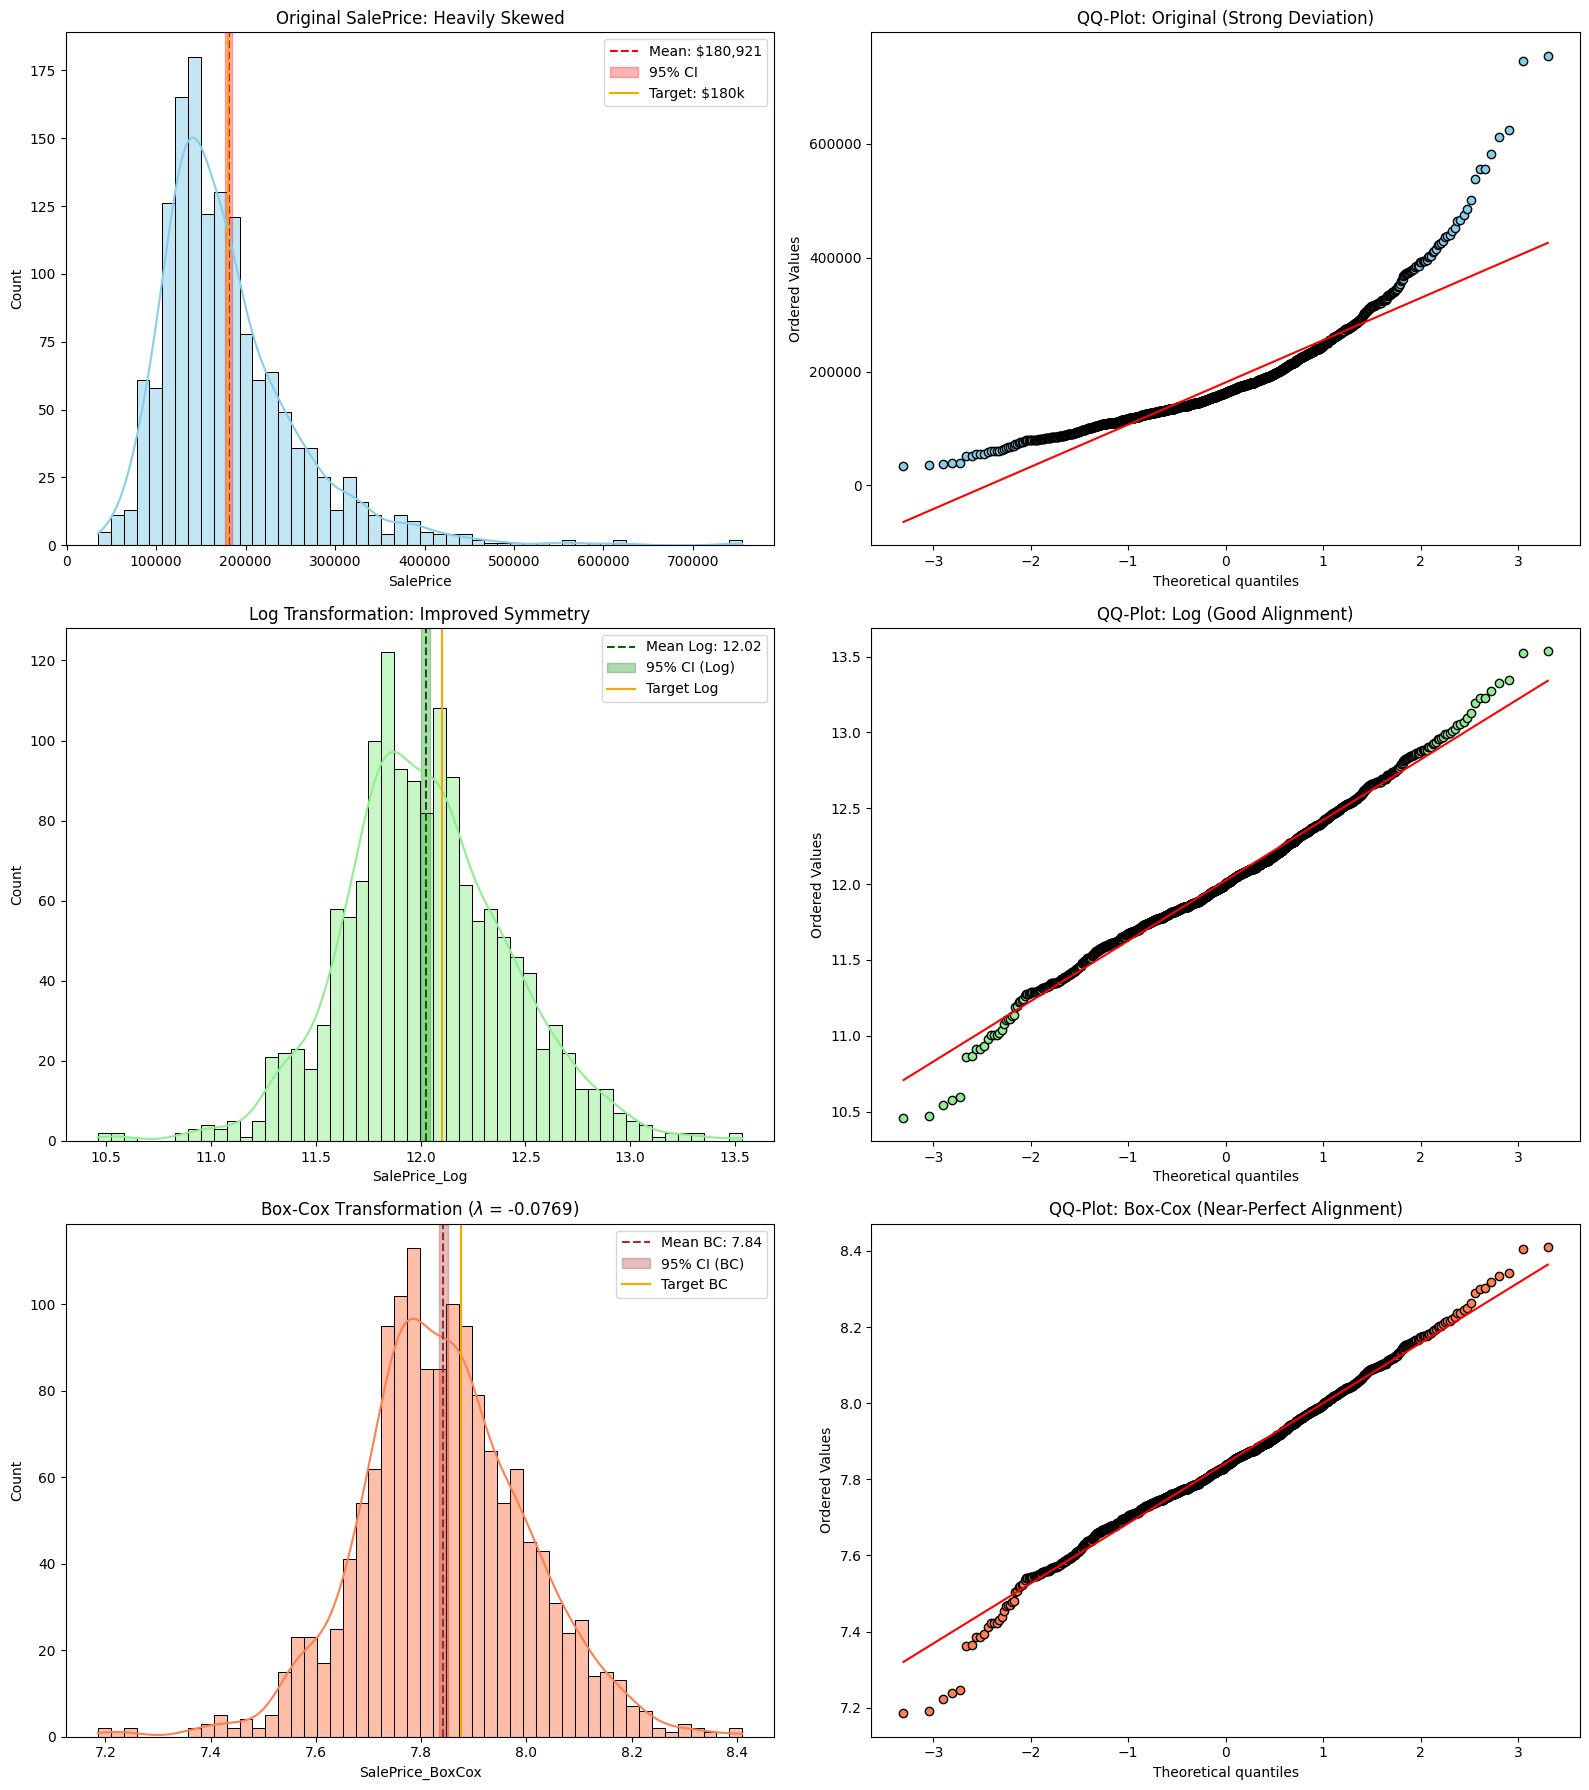
\includegraphics{figures/six_panel_distribution.png}
\caption{Six-panel diagnostic for the three target scales}
\end{figure}

\emph{Figure 3: Six-panel diagnostic for the three target scales. Left
column: histograms with mean (dashed line), 95\% confidence interval
(shaded band), and the \$180,000 reference (orange line). Right column:
QQ-plots against the standard normal distribution. Rows: original
\texttt{SalePrice} (top), \texttt{SalePrice\_Log} (middle),
\texttt{SalePrice\_BoxCox} with \(\lambda = -0.0769\) (bottom).}

\textbf{Comparative analysis of histograms.}

\begin{itemize}
\tightlist
\item
  \textbf{Original \texttt{SalePrice} (Blue) --- Positive Skewness:} the
  initial distribution exhibits highly pronounced right-hand skewness. A
  strong concentration of transactions is observed between \$100k and
  \$200k, while a ``tail'' stretches out to \$750k.
\item
  \textbf{Log Transformation (Green) --- Normalization via Compression:}
  applying the logarithm reduces variance gaps. The distribution now
  adopts a much more balanced bell-curve shape. The peak is better
  centered, and the influence of outliers at the tail of the
  distribution is neutralized.
\item
  \textbf{Box-Cox Transformation (Orange) --- Optimal Symmetry:}
  utilizing an optimized \(\lambda\) (\(-0.0769\)), this method
  outperforms the logarithmic transformation by further tightening the
  extremes. The resulting symmetry is near-perfect.
\end{itemize}

\textbf{Comparative analysis of QQ-plots.}

\begin{itemize}
\tightlist
\item
  \textbf{Original (High Deviation):} a systematic deviation of the data
  points from the bisector (red line) is observed, particularly at the
  extremities. This curvature indicates that the ``tails'' of the actual
  distribution are significantly heavier than those of a normal
  distribution.
\item
  \textbf{Log Transformation (Satisfactory Alignment):} the majority of
  observations now follow the reference line. While slight curvatures
  persist at the extremities (distribution tails), the overall alignment
  is sufficient to consider the variable as following a normal
  distribution for practical application.
\item
  \textbf{Box-Cox (Near-Perfect Alignment):} the Box-Cox transformation
  successfully normalized the center of the data, which closely follows
  the red reference line. However, noticeable deviations at the extremes
  (downward on the left, upward on the right) show the alignment is not
  perfect.
\end{itemize}

\begin{center}\rule{0.5\linewidth}{0.5pt}\end{center}

\subsection{4 ANOVA for Ordinal
Features}\label{anova-for-ordinal-features}

The second part of the project applies ANOVA to determine which of the
ten provided features have a statistically significant effect on the
(transformed) \texttt{SalePrice}. The analysis is conducted on all three
target scales (\texttt{SalePrice}, \texttt{SalePrice\_Log},
\texttt{SalePrice\_BoxCox}) in parallel.

\subsubsection{4.1 Features Analyzed}\label{features-analyzed}

Ten categorical or ordinal features are submitted to the ANOVA analysis.
They are listed in the table below together with their levels and short
description.

\begin{longtable}[]{@{}llll@{}}
\toprule\noalign{}
\# & Feature & Levels & Description \\
\midrule\noalign{}
\endhead
\bottomrule\noalign{}
\endlastfoot
1 & \texttt{OverallQual} & 1--10 & Overall material and finish
quality \\
2 & \texttt{ExterQual} & Po, Fa, TA, Gd, Ex & Exterior material
quality \\
3 & \texttt{BsmtQual} & None, Po, Fa, TA, Gd, Ex & Basement height
quality \\
4 & \texttt{KitchenQual} & Po, Fa, TA, Gd, Ex & Kitchen quality \\
5 & \texttt{FireplaceQu} & None, Po, Fa, TA, Gd, Ex & Fireplace
quality \\
6 & \texttt{CentralAir} & N, Y & Central air conditioning \\
7 & \texttt{LotShape} & IR3, IR2, IR1, Reg & General shape of
property \\
8 & \texttt{LandSlope} & Sev, Mod, Gtl & Slope of property \\
9 & \texttt{MoSold} & 1--12 & Month sold \\
10 & \texttt{YrSold} & 2006--2010 & Year sold \\
\end{longtable}

\emph{Table 5: The ten features submitted to ANOVA analysis, with their
levels and description.}

\subsubsection{4.2 One-Way ANOVA}\label{one-way-anova}

\paragraph{Our approach}\label{our-approach}

\begin{enumerate}
\def\labelenumi{\arabic{enumi}.}
\tightlist
\item
  \textbf{Data inspection (categories):} we first look at the unique
  categories (levels) for each of our 10 features (e.g., checking that
  missing basements have been correctly grouped into a \texttt{None}
  category).
\item
  \textbf{One-Way ANOVA:} we run the ANOVA test for each feature against
  our standard target (\texttt{SalePrice}) as well as our two normalized
  targets (\texttt{SalePrice\_Log} and \texttt{SalePrice\_BoxCox}). This
  allows us to determine which features significantly influence the
  price and to observe how mathematical transformations affect the
  statistical significance.
\end{enumerate}

\paragraph{Results: identifying significant features (p \textless{}
0.05)}\label{results-identifying-significant-features-p-0.05}

The table below reports the F-statistic, p-value, and significance
verdict for each of the ten features across the three target scales. If
\(p < 0.05\), the feature is considered a significant driver of price.

\begin{longtable}[]{@{}
  >{\raggedright\arraybackslash}p{(\columnwidth - 18\tabcolsep) * \real{0.1000}}
  >{\raggedright\arraybackslash}p{(\columnwidth - 18\tabcolsep) * \real{0.1000}}
  >{\raggedright\arraybackslash}p{(\columnwidth - 18\tabcolsep) * \real{0.1000}}
  >{\raggedright\arraybackslash}p{(\columnwidth - 18\tabcolsep) * \real{0.1000}}
  >{\raggedright\arraybackslash}p{(\columnwidth - 18\tabcolsep) * \real{0.1000}}
  >{\raggedright\arraybackslash}p{(\columnwidth - 18\tabcolsep) * \real{0.1000}}
  >{\raggedright\arraybackslash}p{(\columnwidth - 18\tabcolsep) * \real{0.1000}}
  >{\raggedright\arraybackslash}p{(\columnwidth - 18\tabcolsep) * \real{0.1000}}
  >{\raggedright\arraybackslash}p{(\columnwidth - 18\tabcolsep) * \real{0.1000}}
  >{\raggedright\arraybackslash}p{(\columnwidth - 18\tabcolsep) * \real{0.1000}}@{}}
\toprule\noalign{}
\begin{minipage}[b]{\linewidth}\raggedright
Feature
\end{minipage} & \begin{minipage}[b]{\linewidth}\raggedright
F (Orig.)
\end{minipage} & \begin{minipage}[b]{\linewidth}\raggedright
p (Orig.)
\end{minipage} & \begin{minipage}[b]{\linewidth}\raggedright
Sig.
\end{minipage} & \begin{minipage}[b]{\linewidth}\raggedright
F (Log)
\end{minipage} & \begin{minipage}[b]{\linewidth}\raggedright
p (Log)
\end{minipage} & \begin{minipage}[b]{\linewidth}\raggedright
Sig.
\end{minipage} & \begin{minipage}[b]{\linewidth}\raggedright
F (BC)
\end{minipage} & \begin{minipage}[b]{\linewidth}\raggedright
p (BC)
\end{minipage} & \begin{minipage}[b]{\linewidth}\raggedright
Sig.
\end{minipage} \\
\midrule\noalign{}
\endhead
\bottomrule\noalign{}
\endlastfoot
\texttt{OverallQual} & 349.02 & 0.00e+00 & YES & 332.16 & 0.00e+00 & YES
& 325.93 & 0.00e+00 & YES \\
\texttt{ExterQual} & 443.33 & 1.43e-204 & YES & 415.30 & 6.93e-195 & YES
& 406.19 & 1.12e-191 & YES \\
\texttt{BsmtQual} & 316.14 & 8.15e-196 & YES & 300.39 & 2.02e-188 & YES
& 294.55 & 1.23e-185 & YES \\
\texttt{KitchenQual} & 407.80 & 3.03e-192 & YES & 393.32 & 4.43e-187 &
YES & 386.07 & 1.83e-184 & YES \\
\texttt{FireplaceQu} & 121.07 & 2.97e-107 & YES & 131.19 & 6.96e-115 &
YES & 130.06 & 4.88e-114 & YES \\
\texttt{CentralAir} & 98.30 & 1.80e-22 & YES & 205.66 & 9.85e-44 & YES &
215.98 & 1.06e-45 & YES \\
\texttt{LotShape} & 40.13 & 6.44e-25 & YES & 46.72 & 7.85e-29 & YES &
46.63 & 8.89e-29 & YES \\
\texttt{LandSlope} & 1.95 & 0.141 & NO & 1.08 & 0.338 & NO & 0.98 &
0.373 & NO \\
\texttt{MoSold} & 0.95 & 0.483 & NO & 0.99 & 0.449 & NO & 1.00 & 0.443 &
NO \\
\texttt{YrSold} & 0.64 & 0.630 & NO & 0.73 & 0.565 & NO & 0.75 & 0.555 &
NO \\
\end{longtable}

\emph{Table 6: One-Way ANOVA results for the ten features on the three
target scales. Significance is declared at \(\alpha = 0.05\).}

\paragraph{Summary of significant
features}\label{summary-of-significant-features}

The most striking takeaway from the table is that \textbf{transforming
the target variable did not change the final ``True/False'' significance
verdict for a single feature.} Seven features emerge as significant
across all three scales:

\begin{quote}
\texttt{OverallQual}, \texttt{ExterQual}, \texttt{BsmtQual},
\texttt{KitchenQual}, \texttt{FireplaceQu}, \texttt{CentralAir},
\texttt{LotShape}.
\end{quote}

\subsubsection{4.3 Two-Way ANOVA and
Interactions}\label{two-way-anova-and-interactions}

\paragraph{Objective}\label{objective}

Test whether \textbf{two features have a joint effect (interaction) on
the sale price.} For example: does the effect of kitchen quality on
price also depend on the overall quality of the house?

\begin{itemize}
\tightlist
\item
  \textbf{No interaction:} central air conditioning adds \$10,000 to the
  price, regardless of whether the house is low-quality or high-quality.
\item
  \textbf{Interaction:} central air conditioning adds only \$2,000 to a
  low-quality house but \$30,000 to a high-quality house.
\end{itemize}

In the second case the two features ``interact'' because the benefit of
one depends on the level of the other. Operationally, the interaction is
read from the p-value attached to the term \texttt{C(f1):C(f2)} in a
Type II ANOVA table: \(p < 0.05\) means the two features influence the
price jointly, \(p \geq 0.05\) means they act independently. Up to
Section 4.2 we already knew, from One-Way ANOVA, that each of the seven
significant features individually has a significant effect on price. The
entire detour described below is not aimed at re-confirming those main
effects --- it is aimed at unlocking a quantity that One-Way ANOVA
cannot measure: \textbf{the interaction term.}

\paragraph{Why OLS with Type II Sum of
Squares}\label{why-ols-with-type-ii-sum-of-squares}

Two-Way ANOVA can be computed either via the classical manual
Sum-of-Squares formulas or via an OLS regression. We choose OLS for two
concrete reasons.

\textbf{1. Our design is unbalanced.} The classical Two-Way ANOVA
formula was designed for \textbf{balanced designs} --- where every
combination of two features contains exactly the same number of
observations. In our dataset, group sizes are highly unequal (e.g.,
\texttt{OverallQual} level 5 contains hundreds of houses, level 1
contains only 2). The OLS approach combined with Type II Sum of Squares
(\texttt{anova\_lm(model,\ typ=2)}) handles this: it tests each effect
after accounting for all other effects simultaneously, producing
unambiguous results regardless of group sizes.

\textbf{2. The interaction term is natural in a regression formula.} The
classical computation of the interaction Sum of Squares is a cascading
subtraction

\[SS_{\text{interaction}} = SS_{\text{total}} - SS_A - SS_B - SS_{\text{error}}\]

which amplifies rounding errors and becomes complex when categories have
many levels. With OLS, the interaction is directly encoded in the model
formula:

\[Y \sim C(A) + C(B) + C(A):C(B)\]

The term \texttt{C(A):C(B)} creates dummy variables for every
combination of A and B, and the corresponding p-value is read directly
from the ANOVA table.

\paragraph{First attempt: 100\% of pairs are
blocked}\label{first-attempt-100-of-pairs-are-blocked}

We applied the Two-Way ANOVA pipeline to all \(\binom{7}{2} = 21\) pairs
of significant features identified in Section 4.2. Before fitting any
model, the code performs a completeness check on the crosstab of each
pair: any cell with \(N = 0\) (empty combination) or \(N = 1\)
(singleton --- no within-cell variance) blocks the analysis. The
mechanism behind these blockages is mathematical:

\begin{itemize}
\tightlist
\item
  \textbf{Empty cells (\(N = 0\)):} computing the cell mean requires
  dividing by zero observations, which is undefined. The design matrix
  becomes singular and the OLS solver cannot invert it.
\item
  \textbf{Singletons (\(N = 1\)):} the cell mean exists, but the
  within-cell variance formula divides by \(N - 1 = 0\). The F-statistic
  for the interaction term requires this variance, so the test becomes
  undefined.
\end{itemize}

We cannot work around these failures by zero-filling (which would inject
a fake interaction) or by leaving the cells NaN (which would make the
matrix singular).

\begin{figure}
\centering
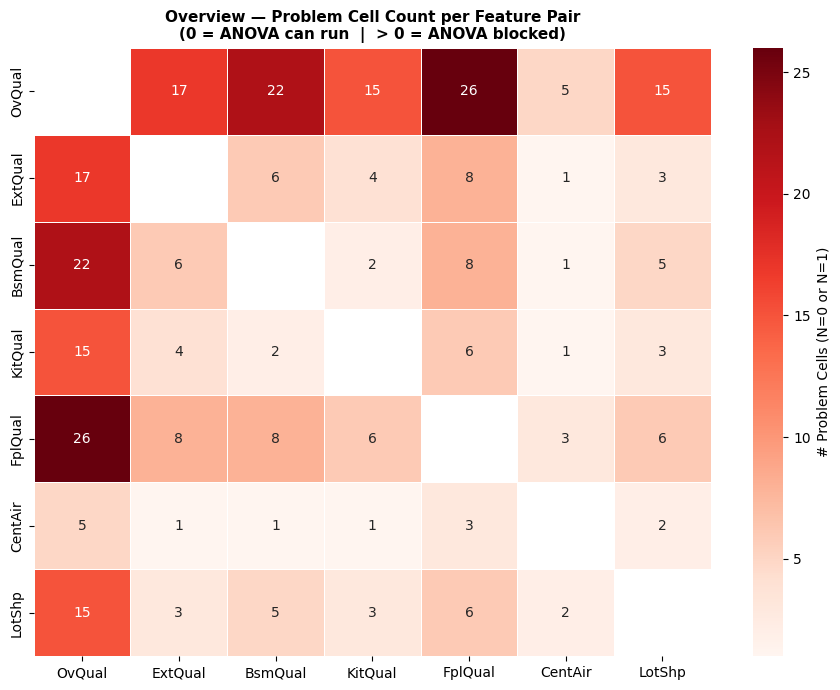
\includegraphics{figures/crosstab_overview.png}
\caption{Overview heatmap of problem cells per feature pair}
\end{figure}

\emph{Figure 4: Overview heatmap of problem cells per feature pair. Each
off-diagonal cell counts the total \(N=0\) plus \(N=1\) combinations
between the two corresponding features. Every pair shows a positive
count, confirming that 100\% of the 21 pairs are blocked.}

Five representative crosstabs (\texttt{OverallQual\ ×\ ExterQual},
\texttt{OverallQual\ ×\ BsmtQual}, \texttt{OverallQual\ ×\ CentralAir},
\texttt{ExterQual\ ×\ KitchenQual}, \texttt{CentralAir\ ×\ LotShape})
are shown in Figures 5--9, with blue cells indicating safe combinations
(\(N \geq 2\)), black cells indicating holes (\(N = 0\)), and red cells
indicating fragile singletons (\(N = 1\)).

\begin{figure}
\centering
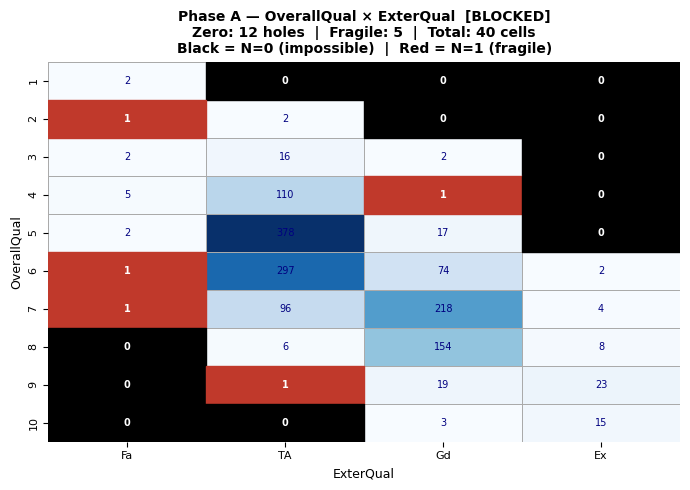
\includegraphics{figures/crosstab_ovqual_extqual.png}
\caption{Crosstab OverallQual × ExterQual}
\end{figure}

\emph{Figure 5: Crosstab OverallQual × ExterQual. Blue cells: safe
(\(N \geq 2\)); black cells with ``0'': empty combinations; red cells
with ``1'': fragile singletons. Pair flagged as {[}BLOCKED{]}.}

\begin{figure}
\centering
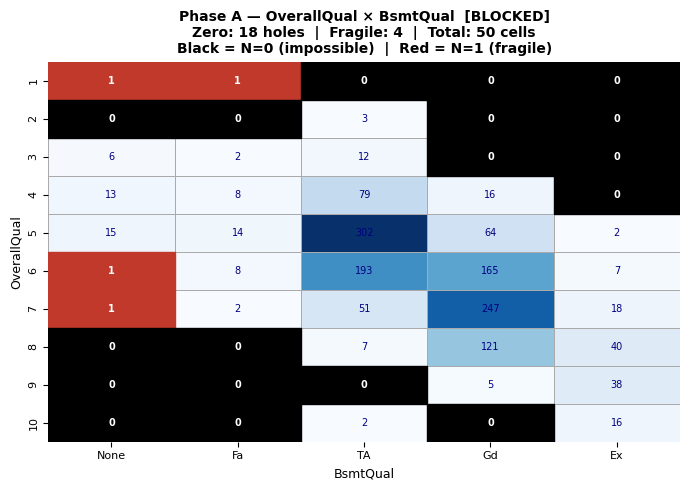
\includegraphics{figures/crosstab_ovqual_bsmqual.png}
\caption{Crosstab OverallQual × BsmtQual}
\end{figure}

\emph{Figure 6: Crosstab OverallQual × BsmtQual. Same colour code as
above. Pair flagged as {[}BLOCKED{]}.}

\begin{figure}
\centering
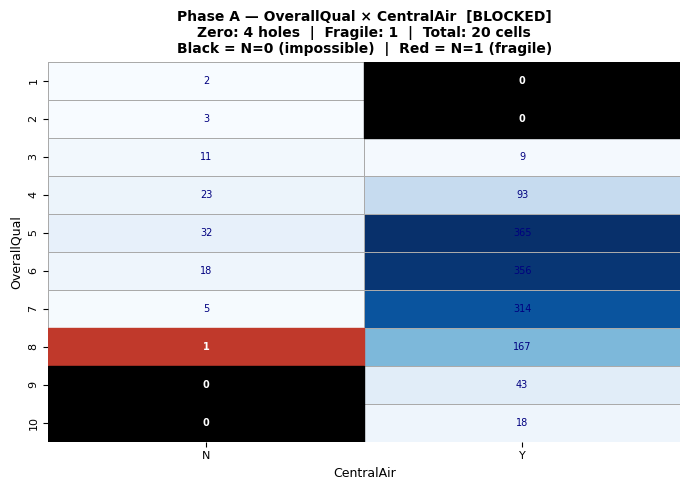
\includegraphics{figures/crosstab_ovqual_centair.png}
\caption{Crosstab OverallQual × CentralAir}
\end{figure}

\emph{Figure 7: Crosstab OverallQual × CentralAir. Same colour code as
above. Pair flagged as {[}BLOCKED{]}.}

\begin{figure}
\centering
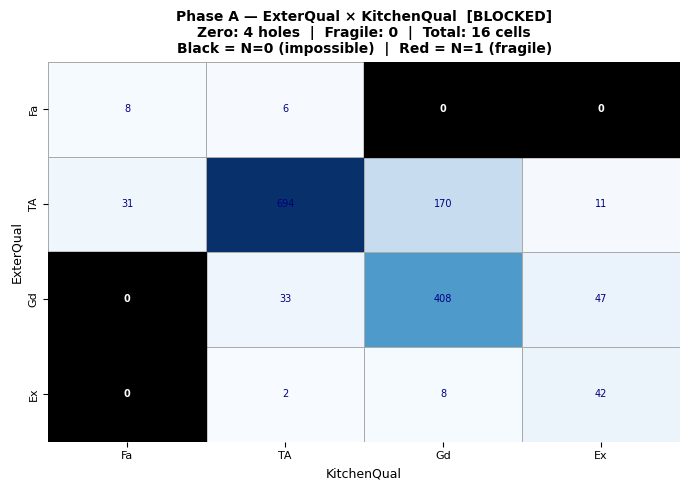
\includegraphics{figures/crosstab_extqual_kitqual.png}
\caption{Crosstab ExterQual × KitchenQual}
\end{figure}

\emph{Figure 8: Crosstab ExterQual × KitchenQual. Same colour code as
above. Pair flagged as {[}BLOCKED{]}.}

\begin{figure}
\centering
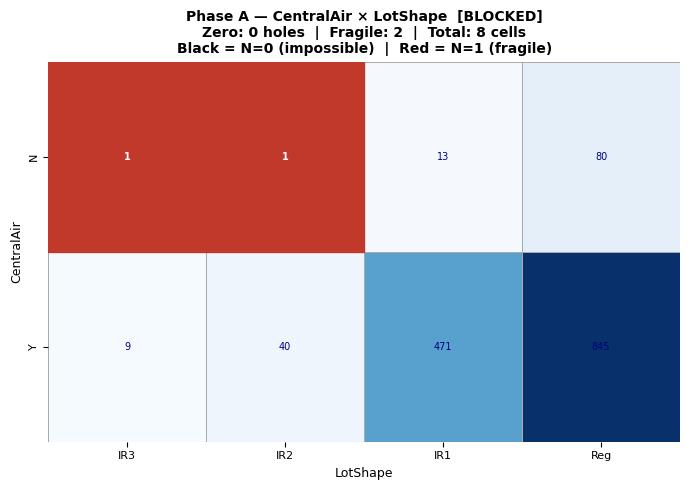
\includegraphics{figures/crosstab_centair_lotshp.png}
\caption{Crosstab CentralAir × LotShape}
\end{figure}

\emph{Figure 9: Crosstab CentralAir × LotShape. Same colour code as
above. Pair flagged as {[}BLOCKED{]}.}

The full severity ranking of the 21 pairs is given in the table below.

\begin{longtable}[]{@{}
  >{\raggedright\arraybackslash}p{(\columnwidth - 12\tabcolsep) * \real{0.1429}}
  >{\raggedright\arraybackslash}p{(\columnwidth - 12\tabcolsep) * \real{0.1429}}
  >{\raggedright\arraybackslash}p{(\columnwidth - 12\tabcolsep) * \real{0.1429}}
  >{\raggedright\arraybackslash}p{(\columnwidth - 12\tabcolsep) * \real{0.1429}}
  >{\raggedright\arraybackslash}p{(\columnwidth - 12\tabcolsep) * \real{0.1429}}
  >{\raggedright\arraybackslash}p{(\columnwidth - 12\tabcolsep) * \real{0.1429}}
  >{\raggedright\arraybackslash}p{(\columnwidth - 12\tabcolsep) * \real{0.1429}}@{}}
\toprule\noalign{}
\begin{minipage}[b]{\linewidth}\raggedright
\#
\end{minipage} & \begin{minipage}[b]{\linewidth}\raggedright
Pair
\end{minipage} & \begin{minipage}[b]{\linewidth}\raggedright
Total Cells
\end{minipage} & \begin{minipage}[b]{\linewidth}\raggedright
Holes (N=0)
\end{minipage} & \begin{minipage}[b]{\linewidth}\raggedright
Fragile (N=1)
\end{minipage} & \begin{minipage}[b]{\linewidth}\raggedright
Problems
\end{minipage} & \begin{minipage}[b]{\linewidth}\raggedright
Status
\end{minipage} \\
\midrule\noalign{}
\endhead
\bottomrule\noalign{}
\endlastfoot
0 & \texttt{OverallQual\ ×\ FireplaceQu} & 60 & 22 & 4 & 26 &
{[}BLOCKED{]} \\
1 & \texttt{OverallQual\ ×\ BsmtQual} & 50 & 18 & 4 & 22 &
{[}BLOCKED{]} \\
2 & \texttt{OverallQual\ ×\ ExterQual} & 40 & 12 & 5 & 17 &
{[}BLOCKED{]} \\
3 & \texttt{OverallQual\ ×\ KitchenQual} & 40 & 12 & 3 & 15 &
{[}BLOCKED{]} \\
4 & \texttt{OverallQual\ ×\ LotShape} & 40 & 10 & 5 & 15 &
{[}BLOCKED{]} \\
5 & \texttt{BsmtQual\ ×\ FireplaceQu} & 30 & 6 & 2 & 8 &
{[}BLOCKED{]} \\
6 & \texttt{ExterQual\ ×\ FireplaceQu} & 24 & 6 & 2 & 8 &
{[}BLOCKED{]} \\
7 & \texttt{FireplaceQu\ ×\ LotShape} & 24 & 3 & 3 & 6 &
{[}BLOCKED{]} \\
8 & \texttt{ExterQual\ ×\ BsmtQual} & 20 & 3 & 3 & 6 & {[}BLOCKED{]} \\
9 & \texttt{KitchenQual\ ×\ FireplaceQu} & 24 & 5 & 1 & 6 &
{[}BLOCKED{]} \\
10 & \texttt{OverallQual\ ×\ CentralAir} & 20 & 4 & 1 & 5 &
{[}BLOCKED{]} \\
11 & \texttt{BsmtQual\ ×\ LotShape} & 20 & 3 & 2 & 5 & {[}BLOCKED{]} \\
12 & \texttt{ExterQual\ ×\ KitchenQual} & 16 & 4 & 0 & 4 &
{[}BLOCKED{]} \\
13 & \texttt{FireplaceQu\ ×\ CentralAir} & 12 & 2 & 1 & 3 &
{[}BLOCKED{]} \\
14 & \texttt{KitchenQual\ ×\ LotShape} & 16 & 2 & 1 & 3 &
{[}BLOCKED{]} \\
15 & \texttt{ExterQual\ ×\ LotShape} & 16 & 1 & 2 & 3 & {[}BLOCKED{]} \\
16 & \texttt{BsmtQual\ ×\ KitchenQual} & 20 & 2 & 0 & 2 &
{[}BLOCKED{]} \\
17 & \texttt{CentralAir\ ×\ LotShape} & 8 & 0 & 2 & 2 & {[}BLOCKED{]} \\
18 & \texttt{ExterQual\ ×\ CentralAir} & 8 & 1 & 0 & 1 &
{[}BLOCKED{]} \\
19 & \texttt{KitchenQual\ ×\ CentralAir} & 8 & 0 & 1 & 1 &
{[}BLOCKED{]} \\
20 & \texttt{BsmtQual\ ×\ CentralAir} & 10 & 1 & 0 & 1 &
{[}BLOCKED{]} \\
\end{longtable}

\emph{Table 7: Severity summary of the 21 feature pairs, sorted by total
number of problem cells. The full grid is blocked: even the least severe
pairs at the bottom contain at least one problem cell, which is enough
to block the test.}

The root cause is \textbf{structural rather than methodological.} The
dataset is \textbf{observational}: certain quality combinations simply
do not exist in the housing market (a house with overall quality ``Very
Poor'' and an ``Excellent'' fireplace, for example). Classical Two-Way
ANOVA was designed for controlled experimental designs where all
combinations are guaranteed by construction; observational data does not
satisfy this prerequisite.

\paragraph{Two naive approaches and why they
fail}\label{two-naive-approaches-and-why-they-fail}

Before designing the pipeline, we considered two simpler strategies and
rejected both.

\textbf{Approach 1 --- Dropping rare sub-categories.} The idea is to
remove the levels that create empty cells (e.g., drop \texttt{Po} and
\texttt{Fa} from \texttt{FireplaceQu} because too few houses fall into
those categories). This causes real information loss and biases the
results: dropping ``Poor'' and ``Fair'' means analysing only
average-to-excellent quality houses, so the model no longer represents
the full market. Conclusions would be valid only on a subset of the
data, making them non-generalisable.

\textbf{Approach 2 --- Naive merging (the small-sample trap).} The idea
is to merge rare levels with their neighbours to fill the empty cells,
based purely on a t-test of mean equality. This falls into a subtle but
systematic trap.

Consider \texttt{FireplaceQu} on \texttt{SalePrice\_Log}: ``Po'' has
\(N = 3\), mean = 11.80, \(\sigma = 0.41\); ``Fa'' has \(N = 28\), mean
= 11.85, \(\sigma = 0.38\). The gap between means is only 0.05, the
t-test returns \(p = 0.72\), and a naive reading would conclude
``compatible, safe to merge''. But the 95\% confidence interval on the
true mean of ``Po'' is

\[11.80 \pm 2.92 \times \frac{0.41}{\sqrt{3}} = [11.11, 12.49],\]

so the true mean of ``Poor'' could plausibly be as high as 12.3 --- a
real gap of \(+0.45\) against ``Fair'', equivalent to a
\textasciitilde45\% price difference. The t-test fails to detect this
gap not because it does not exist, but because \(N = 3\) gives the test
no statistical power. The problem is systematic in our dataset: the rare
sub-categories (the ones causing empty cells) are exactly those with low
\(N\). The merging approach therefore falls into a vicious cycle --- the
categories that need merging are precisely those for which merging is
statistically unreliable.

We need a strategy that (i) merges only when the indistinguishability is
detected with appropriate multiple-testing protection, and (ii) refuses
to merge when doing so would violate the ordinal or categorical
structure of the variable. This motivates the 4-cell pipeline below.

\paragraph{The escape route: a 4-cell
pipeline}\label{the-escape-route-a-4-cell-pipeline}

Rather than abandon the Two-Way ANOVA, we implement an
\textbf{intelligent binning strategy}: merge ordinally adjacent levels
that the data cannot distinguish, in order to refill the empty cells.
The pipeline runs in four cells:

\begin{enumerate}
\def\labelenumi{\arabic{enumi}.}
\tightlist
\item
  \textbf{Cell A --- Tukey HSD:} map every pairwise within-feature
  difference and flag which level pairs are statistically
  indistinguishable.
\item
  \textbf{Cell B --- Rule-based filter:} keep only the merge candidates
  that are both non-significant in Tukey and structurally meaningful (no
  fusing of non-adjacent levels, no fusing of a binary variable, no
  fusing across nominal macro-families).
\item
  \textbf{Cell C --- Union-Find fusion + diagnostic:} apply the filtered
  candidates as a transitive equivalence relation on the levels of each
  feature, then recompute the crosstabs to see which pairs are now
  unblocked.
\item
  \textbf{Cell D --- Two-Way ANOVA:} run the OLS test on the pairs that
  survived, skip the rest with an explicit reason.
\end{enumerate}

The pipeline is repeated independently on the three target scales
(\texttt{SalePrice}, \texttt{SalePrice\_Log},
\texttt{SalePrice\_BoxCox}), since the choice of scale affects which
levels Tukey considers indistinguishable and therefore which fusions are
produced.

\textbf{Cell A --- Tukey HSD.} Tukey's Honestly Significant Difference
test compares the means of every pair of levels within a feature
(e.g.~all 45 pairs for the 10 levels of \texttt{OverallQual}), and
returns a family-wise-corrected p-value for each comparison. The
correction matters: running many comparisons at once inflates the
false-positive rate; Tukey controls the family-wise error rate, so the
verdict on each pair stays reliable even when dozens of tests are run
together. This is precisely the protection that the naive t-test in
Approach 2 lacks.

For each pair we obtain a \texttt{meandiff} (gap between the two group
means), a \texttt{p-adj} (family-wise-corrected p-value), and a
\texttt{reject} verdict (\(H_0\) rejected or not). A non-significant
pair (\(p \geq 0.05\)) is a candidate for merging; a significant pair
must never be merged.

Because the same statistical information is read on three scales with
very different units, we format \texttt{meandiff} differently per target
to keep the output legible: dollars for \texttt{SalePrice}; log units
with a percentage equivalent \(e^\Delta - 1\) for
\texttt{SalePrice\_Log}; raw value to six decimals for
\texttt{SalePrice\_BoxCox} (the Box-Cox scale has no intuitive
interpretation since \(\lambda \approx -0.0769\)). The table below
consolidates the pair counts across the three target scales.

\begin{longtable}[]{@{}
  >{\raggedright\arraybackslash}p{(\columnwidth - 14\tabcolsep) * \real{0.1250}}
  >{\raggedright\arraybackslash}p{(\columnwidth - 14\tabcolsep) * \real{0.1250}}
  >{\raggedright\arraybackslash}p{(\columnwidth - 14\tabcolsep) * \real{0.1250}}
  >{\raggedright\arraybackslash}p{(\columnwidth - 14\tabcolsep) * \real{0.1250}}
  >{\raggedright\arraybackslash}p{(\columnwidth - 14\tabcolsep) * \real{0.1250}}
  >{\raggedright\arraybackslash}p{(\columnwidth - 14\tabcolsep) * \real{0.1250}}
  >{\raggedright\arraybackslash}p{(\columnwidth - 14\tabcolsep) * \real{0.1250}}
  >{\raggedright\arraybackslash}p{(\columnwidth - 14\tabcolsep) * \real{0.1250}}@{}}
\toprule\noalign{}
\begin{minipage}[b]{\linewidth}\raggedright
Feature
\end{minipage} & \begin{minipage}[b]{\linewidth}\raggedright
Total Pairs
\end{minipage} & \begin{minipage}[b]{\linewidth}\raggedright
Sig. (Orig.)
\end{minipage} & \begin{minipage}[b]{\linewidth}\raggedright
Non-Sig. (Orig.)
\end{minipage} & \begin{minipage}[b]{\linewidth}\raggedright
Sig. (Log)
\end{minipage} & \begin{minipage}[b]{\linewidth}\raggedright
Non-Sig. (Log)
\end{minipage} & \begin{minipage}[b]{\linewidth}\raggedright
Sig. (BC)
\end{minipage} & \begin{minipage}[b]{\linewidth}\raggedright
Non-Sig. (BC)
\end{minipage} \\
\midrule\noalign{}
\endhead
\bottomrule\noalign{}
\endlastfoot
\texttt{OverallQual} & 45 & 37 & 8 & 43 & 2 & 43 & 2 \\
\texttt{ExterQual} & 6 & 6 & 0 & 6 & 0 & 6 & 0 \\
\texttt{BsmtQual} & 10 & 8 & 2 & 9 & 1 & 9 & 1 \\
\texttt{KitchenQual} & 6 & 6 & 0 & 6 & 0 & 6 & 0 \\
\texttt{FireplaceQu} & 15 & 12 & 3 & 13 & 2 & 13 & 2 \\
\texttt{CentralAir} & 1 & 1 & 0 & 1 & 0 & 1 & 0 \\
\texttt{LotShape} & 6 & 3 & 3 & 2 & 4 & 2 & 4 \\
\textbf{TOTAL} & \textbf{89} & \textbf{73} & \textbf{16} & \textbf{80} &
\textbf{9} & \textbf{80} & \textbf{9} \\
\end{longtable}

\emph{Table 8: Tukey HSD pair counts per feature on the three target
scales. ``Non-Sig.'' counts the raw merge candidates before structural
filtering.}

Two observations stand out. First, \textbf{transforming the target
dramatically reduces the number of non-significant pairs} --- from 16 on
the original scale down to 9 on both Log and Box-Cox. The mechanism is
the heavy variance within high-quality groups on the original scale (a
single
\(750k outlier in the `OverallQual = 9` group inflates the standard error), which Tukey's test compares against the gap between means; once the scale is normalised the variance shrinks and previously hidden differences become detectable. Second, Log and Box-Cox produce nearly identical verdicts on every feature, consistent with the fact that the optimal Box-Cox parameter (\)\lambda \approx -0.0769\$)
is close to 0 --- the value at which Box-Cox becomes a logarithm.

\textbf{Cell B --- Rule-based filter.} Tukey alone tells us which means
are statistically indistinguishable, but it does not tell us whether
merging them is structurally meaningful. Blindly merging on p-values
alone leads to two failure modes: destroying ordinal structure (merging
``Poor'' with ``Excellent'' just because their sample means happened to
be close) and collapsing categorical semantics. We therefore enforce
three rules in addition to the Tukey verdict.

\begin{itemize}
\tightlist
\item
  \textbf{Rule 1 --- Ordinal Proximity (for ordinal features).} For
  features with a natural ordering (\texttt{OverallQual} 1→10,
  \texttt{ExterQual}/\texttt{KitchenQual} Po→Ex,
  \texttt{BsmtQual}/\texttt{FireplaceQu} None→Ex), only \textbf{adjacent
  pairs} on the scale are eligible. Merging \texttt{Po} with \texttt{Fa}
  is acceptable (direct neighbours on a quality ladder); merging
  \texttt{Po} with \texttt{Ex} is forbidden, because it would create a
  group spanning the entire quality range with no real-world meaning.
  This rule preserves the monotonic relationship between quality level
  and price that justified treating these features as ordinal in the
  first place.
\item
  \textbf{Rule 2 --- Binary Lock (for binary features).} The variable
  \texttt{CentralAir} has only two levels (N, Y). Merging them would
  eliminate the variable entirely: a feature with a single level carries
  zero information. Even if Tukey returned a non-significant verdict,
  fusion would be analytically nonsensical. \texttt{CentralAir} is
  therefore marked as \textbf{untouchable}: no pair is eligible.
\item
  \textbf{Rule 3 --- Nominal Macro-Families (for nominal features).}
  \texttt{LotShape} is the only non-ordinal feature in the set. Its four
  levels (Reg, IR1, IR2, IR3) split naturally into two semantic
  families: \textbf{Reg} (regular rectangular lot) versus
  \textbf{IR1/IR2/IR3} (progressively more irregular shapes). Eligible
  pairs are restricted to those within the same macro-family --- any
  pair among \{IR1, IR2, IR3\} is allowed, but no irregular level may
  ever be merged with \texttt{Reg}.
\item
  \textbf{Rule 4 --- Handling \texttt{None} (automatic).} Some features
  (\texttt{BsmtQual}, \texttt{FireplaceQu}) include a \texttt{None}
  level representing the absence of the feature. We place \texttt{None}
  at the bottom of the ordinal scale, so Rule 1 automatically applies:
  \texttt{None} is adjacent only to the lowest quality level
  (\texttt{Po}).
\end{itemize}

A pair becomes a merge candidate if and only if it satisfies both
eligibility (R1, R2, or R3) and non-significance in Tukey. The table
below shows the final candidate counts after applying the filter.

\begin{longtable}[]{@{}llll@{}}
\toprule\noalign{}
Feature & SalePrice & SalePrice\_Log & SalePrice\_BoxCox \\
\midrule\noalign{}
\endhead
\bottomrule\noalign{}
\endlastfoot
\texttt{OverallQual} & 3 & 2 & 2 \\
\texttt{ExterQual} & 0 & 0 & 0 \\
\texttt{BsmtQual} & 2 & 1 & 1 \\
\texttt{KitchenQual} & 0 & 0 & 0 \\
\texttt{FireplaceQu} & 2 & 2 & 2 \\
\texttt{CentralAir} & 0 & 0 & 0 \\
\texttt{LotShape} & 2 & 3 & 3 \\
\textbf{TOTAL} & \textbf{9} & \textbf{8} & \textbf{8} \\
\end{longtable}

\emph{Table 9: Final merge candidates per feature and target, after
applying the three structural rules. Three features (\texttt{ExterQual},
\texttt{KitchenQual}, \texttt{CentralAir}) produce zero candidates on
all three targets and will pass through to the fusion step unchanged.}

The structural filter has the biggest effect on the original scale: of
the 16 raw non-significant pairs returned by Tukey, only 9 survive. The
cuts come almost entirely from \texttt{OverallQual} --- pairs like (1,
3), (1, 4), (1, 5), (2, 4), (2, 5) are non-adjacent and are blocked by
Rule 1. On the transformed scales, almost no candidate is wasted (8 of 9
raw candidates survive), which is consistent with the fact that the
transformations naturally yield Tukey-non-significant pairs at the
extremes of each scale (e.g.~adjacent pairs like (1, 2) and (9, 10) on
\texttt{OverallQual}).

\textbf{Cell C --- Union-Find fusion and post-merge diagnostic.} The
merge candidates returned by Cell B are individual pairs, but they chain
together. For example, on \texttt{SalePrice}, the candidates for
\texttt{OverallQual} include (1, 2), (2, 3), (3, 4). Taken pair by pair
these describe local indistinguishability; together they form a
\textbf{transitive equivalence relation} that groups the four levels
into a single class \(\{1, 2, 3, 4\}\). We need an algorithm that
respects this transitivity rather than producing three disjoint
pairings, which would be analytically incoherent.

We use the standard \textbf{Union-Find algorithm}:

\begin{itemize}
\tightlist
\item
  Initialise a \texttt{parent} mapping where every level points to
  itself.
\item
  For every candidate pair \((a, b)\), call \texttt{union(a,\ b)} to
  link the two groups containing \(a\) and \(b\).
\item
  After processing all candidates, the connected components of the graph
  define the merged classes. Each class is labelled with a canonical
  name built by joining its members in ordinal order
  (e.g.~\texttt{1+2+3+4}, \texttt{Fa+None}, \texttt{IR1+IR2+IR3}).
\end{itemize}

\textbf{Fusion is a hopeful operation, not a guaranteed one.} Two
structural reasons explain why the Two-Way ANOVA can remain blocked even
after merging. First, no candidates means no fusion: three of the seven
features (\texttt{ExterQual}, \texttt{KitchenQual}, \texttt{CentralAir})
produced zero merge candidates on all three targets, so their level
structure stays exactly as it was, and any feature pair involving one of
them inherits the same empty cells as before. Second, even where
candidates exist, they only collapse levels that Tukey \textbf{failed}
to distinguish; if a feature has empty cells caused by levels that Tukey
did distinguish (which we are forbidden from merging), those cells
persist. The post-fusion diagnostic is therefore not a formality --- it
is the only way to know, pair by pair, where the Two-Way ANOVA in Cell D
becomes runnable.

The table below shows the equivalence classes produced for each feature
on each target.

\begin{longtable}[]{@{}
  >{\raggedright\arraybackslash}p{(\columnwidth - 6\tabcolsep) * \real{0.2500}}
  >{\raggedright\arraybackslash}p{(\columnwidth - 6\tabcolsep) * \real{0.2500}}
  >{\raggedright\arraybackslash}p{(\columnwidth - 6\tabcolsep) * \real{0.2500}}
  >{\raggedright\arraybackslash}p{(\columnwidth - 6\tabcolsep) * \real{0.2500}}@{}}
\toprule\noalign{}
\begin{minipage}[b]{\linewidth}\raggedright
Feature
\end{minipage} & \begin{minipage}[b]{\linewidth}\raggedright
SalePrice
\end{minipage} & \begin{minipage}[b]{\linewidth}\raggedright
SalePrice\_Log
\end{minipage} & \begin{minipage}[b]{\linewidth}\raggedright
SalePrice\_BoxCox
\end{minipage} \\
\midrule\noalign{}
\endhead
\bottomrule\noalign{}
\endlastfoot
\texttt{OverallQual} & {[}1+2+3+4{]} & {[}1+2{]}, {[}9+10{]} &
{[}1+2{]}, {[}9+10{]} \\
\texttt{ExterQual} & --- (no change) & --- (no change) & --- (no
change) \\
\texttt{BsmtQual} & {[}None+Fa+TA{]} & {[}None+Fa{]} & {[}None+Fa{]} \\
\texttt{KitchenQual} & --- (no change) & --- (no change) & --- (no
change) \\
\texttt{FireplaceQu} & {[}None+Po+Fa{]} & {[}None+Po{]}, {[}TA+Gd{]} &
{[}None+Po{]}, {[}TA+Gd{]} \\
\texttt{CentralAir} & --- (locked by R2) & --- (locked by R2) & ---
(locked by R2) \\
\texttt{LotShape} & {[}IR3+IR2+IR1{]} & {[}IR3+IR2+IR1{]} &
{[}IR3+IR2+IR1{]} \\
\end{longtable}

\emph{Table 10: Applied fusions per feature and target, after
Union-Find. The original scale produces aggressive 3- and 4-level chains
on \texttt{OverallQual}, \texttt{BsmtQual}, and \texttt{FireplaceQu};
the transformed scales produce more cautious 2-level fusions at the
extremes.}

After fusion, we re-compute the 21 crosstabs on each target to count
residual empty cells and singletons.

\begin{figure}
\centering
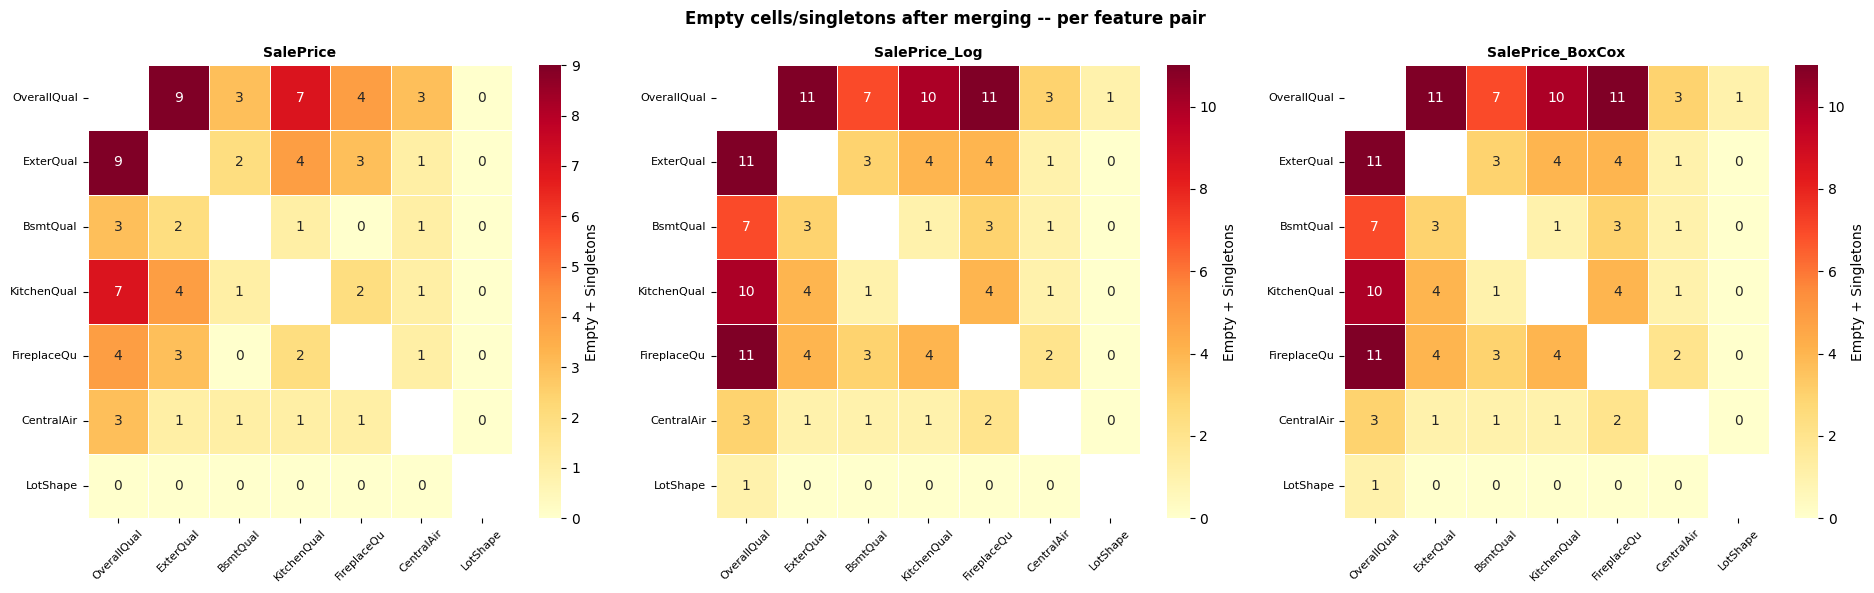
\includegraphics{figures/post_merge_heatmaps.png}
\caption{Empty cells plus singletons after merging}
\end{figure}

\emph{Figure 10: Empty cells plus singletons after merging, per feature
pair, on the three target scales. A value of 0 means the pair is now
unblocked and can be tested via Two-Way ANOVA. On \texttt{SalePrice},
the \texttt{LotShape} row and column are entirely zero. On
\texttt{SalePrice\_Log} and \texttt{SalePrice\_BoxCox}, the
\texttt{LotShape} row and column are also nearly zero (a single residual
singleton on \texttt{OverallQual\ ×\ LotShape}). The
\texttt{OverallQual} row remains the most saturated on the transformed
scales.}

The fusion strategy partially succeeded: \texttt{LotShape}-anchored
pairs are fully unblocked on every target (consequence of the aggressive
3-level fusion \texttt{{[}IR3+IR2+IR1{]}}), and a few additional pairs
are unblocked on the original scale thanks to the 4-level fusion
\texttt{{[}1+2+3+4{]}} on \texttt{OverallQual}. The original scale ends
up with \textbf{7 testable pairs out of 21}; the Log and Box-Cox scales
end up with \textbf{5 each}, leaving 38 and 73 residual problem cells
respectively.

\textbf{A counter-intuitive result: the original scale outperforms the
transformed scales at this step.} The transformed scales have been
consistently better than the original throughout the Tukey analysis
(more pairs detected as significant, cleaner separability). Yet here the
original ends up with roughly half the residual problem cells. The
mechanism is structural, not statistical. The original scale produced an
aggressive 4-level fusion on \texttt{OverallQual}
(\texttt{{[}1+2+3+4{]}}), while Log/BoxCox produced two cautious 2-level
fusions (\texttt{{[}1+2{]}} and \texttt{{[}9+10{]}}). This difference
comes from how Tukey behaved on each scale: on the original, the test
failed to separate 8 low-end pairs because the variance was inflated by
outliers, so many of them survived the structural filter as candidates.
On Log/BoxCox, the compressed variance restored separability across the
middle of the scale, leaving only the extremes as non-significant. Tukey
was therefore ``more correct'' on the transformed scales --- but its
correctness translated into fewer fusions, which means more surviving
levels, which means more crosstab cells, which means more opportunities
for emptiness. Two-Way ANOVA needs \textbf{density}, not
\textbf{discrimination}; the original scale's over-merging is a
statistical compromise that pays off in operational feasibility.

\textbf{Cell D --- Two-Way ANOVA on the unblocked pairs.} For each pair
that survived the diagnostic, we fit the OLS model

\[\text{target} \sim C(f_1) + C(f_2) + C(f_1):C(f_2)\]

on the fused dataframe, and read the interaction p-value from row
\texttt{C(f1):C(f2)} of the Type II ANOVA table. Pairs that did not
survive are skipped with an explicit reason
(\texttt{SKIP\ (n\ empty\ cell(s))} or
\texttt{SKIP\ (n\ singleton(s))}). The two skip conditions are reported
separately so the failure mode is diagnosable: empty cells make the
design matrix singular, while singletons make the within-cell variance
undefined. Significance is coded with the conventional stars:
\texttt{***} for \(p < 0.001\), \texttt{**} for \(p < 0.01\), \texttt{*}
for \(p < 0.05\), \texttt{.} for \(p < 0.10\).

\paragraph{Results}\label{results}

The table below gives the overall counts of tested pairs and significant
interactions on each scale.

\begin{longtable}[]{@{}
  >{\raggedright\arraybackslash}p{(\columnwidth - 8\tabcolsep) * \real{0.2000}}
  >{\raggedright\arraybackslash}p{(\columnwidth - 8\tabcolsep) * \real{0.2000}}
  >{\raggedright\arraybackslash}p{(\columnwidth - 8\tabcolsep) * \real{0.2000}}
  >{\raggedright\arraybackslash}p{(\columnwidth - 8\tabcolsep) * \real{0.2000}}
  >{\raggedright\arraybackslash}p{(\columnwidth - 8\tabcolsep) * \real{0.2000}}@{}}
\toprule\noalign{}
\begin{minipage}[b]{\linewidth}\raggedright
Target
\end{minipage} & \begin{minipage}[b]{\linewidth}\raggedright
Tested / Total
\end{minipage} & \begin{minipage}[b]{\linewidth}\raggedright
Skipped
\end{minipage} & \begin{minipage}[b]{\linewidth}\raggedright
Sig. (p \textless{} 0.05)
\end{minipage} & \begin{minipage}[b]{\linewidth}\raggedright
Borderline (0.05 ≤ p \textless{} 0.10)
\end{minipage} \\
\midrule\noalign{}
\endhead
\bottomrule\noalign{}
\endlastfoot
\texttt{SalePrice} & 7 / 21 & 14 & 3 & 1 \\
\texttt{SalePrice\_Log} & 5 / 21 & 16 & 3 & 0 \\
\texttt{SalePrice\_BoxCox} & 5 / 21 & 16 & 3 & 0 \\
\end{longtable}

\emph{Table 11: Two-Way ANOVA outcome per target. Each scale yields
exactly 3 significant interactions. Main effects (\texttt{C(f1)} and
\texttt{C(f2)}) were massively significant (\(p < 0.001\)) on every
tested pair, re-confirming the One-Way ANOVA verdicts of Section 4.2.}

The table below consolidates every interaction found significant on at
least one target.

\begin{longtable}[]{@{}
  >{\raggedright\arraybackslash}p{(\columnwidth - 6\tabcolsep) * \real{0.2500}}
  >{\raggedright\arraybackslash}p{(\columnwidth - 6\tabcolsep) * \real{0.2500}}
  >{\raggedright\arraybackslash}p{(\columnwidth - 6\tabcolsep) * \real{0.2500}}
  >{\raggedright\arraybackslash}p{(\columnwidth - 6\tabcolsep) * \real{0.2500}}@{}}
\toprule\noalign{}
\begin{minipage}[b]{\linewidth}\raggedright
Pair
\end{minipage} & \begin{minipage}[b]{\linewidth}\raggedright
SalePrice
\end{minipage} & \begin{minipage}[b]{\linewidth}\raggedright
SalePrice\_Log
\end{minipage} & \begin{minipage}[b]{\linewidth}\raggedright
SalePrice\_BoxCox
\end{minipage} \\
\midrule\noalign{}
\endhead
\bottomrule\noalign{}
\endlastfoot
\texttt{OverallQual\ ×\ LotShape} & F = 3.21, p = 0.0039 ** & SKIP
(singleton) & SKIP (singleton) \\
\texttt{ExterQual\ ×\ LotShape} & F = 2.92, p = 0.0332 * & F = 4.20, p =
0.0057 ** & F = 4.30, p = 0.0050 ** \\
\texttt{BsmtQual\ ×\ FireplaceQu} & F = 8.52, p \textless{} 0.0001 *** &
SKIP (empty) & SKIP (empty) \\
\texttt{BsmtQual\ ×\ LotShape} & F = 0.24, p = 0.7879 & F = 3.28, p =
0.0202 * & F = 3.43, p = 0.0165 * \\
\texttt{KitchenQual\ ×\ LotShape} & F = 2.00, p = 0.1117 & F = 4.79, p =
0.0025 ** & F = 5.07, p = 0.0017 ** \\
\texttt{FireplaceQu\ ×\ LotShape} & F = 2.13, p = 0.0945 . & F = 0.62, p
= 0.6029 & F = 0.57, p = 0.6356 \\
\texttt{CentralAir\ ×\ LotShape} & F = 0.49, p = 0.4824 & F = 0.30, p =
0.5833 & F = 0.28, p = 0.5969 \\
\end{longtable}

\emph{Table 12: All Two-Way ANOVA verdicts on tested pairs. Only
\texttt{ExterQual\ ×\ LotShape} is significant on all three targets
simultaneously.}

Three patterns emerge across the cross-target comparison.

\textbf{\texttt{LotShape} is the structural hub of every detected
interaction.} Out of the 9 significant-interaction verdicts across the
three targets, 8 involve \texttt{LotShape} (the exception is
\texttt{BsmtQual\ ×\ FireplaceQu} on the original scale). This is the
direct mechanical consequence of Cell C: \texttt{LotShape} was the only
feature where the fusion strategy fully unlocked the matrix (collapse of
the irregular family), so every pair involving \texttt{LotShape} becomes
testable. The analysis therefore tells us about interactions with lot
shape specifically, not about interactions in general --- the structural
limitation of the data filters the type of insight we can extract.

\textbf{The original scale unlocks a unique interaction:
\texttt{BsmtQual\ ×\ FireplaceQu}.} This pair is the strongest
interaction detected in the entire analysis (\(F = 8.52\),
\(p < 0.0001\)), but it appears only on the original scale. The reason
is again structural: on the original scale, the aggressive 3-level
fusions \texttt{{[}None+Fa+TA{]}} on \texttt{BsmtQual} and
\texttt{{[}None+Po+Fa{]}} on \texttt{FireplaceQu} shrank the crosstab
enough to fully resolve it; on Log and Box-Cox, the cautious 2-level
merges left this crosstab still fragmented. This is a concrete case
where the original scale provides analytical access that the transformed
scales lose. The interaction is real and economically interpretable: the
joint presence or absence of a quality basement and a quality fireplace
creates a price premium beyond their additive contributions.

\textbf{Log/BoxCox reveal interactions hidden by original-scale
variance.} Two pairs --- \texttt{BsmtQual\ ×\ LotShape} and
\texttt{KitchenQual\ ×\ LotShape} --- are clearly non-significant on the
original scale (\(p = 0.79\) and \(p = 0.11\)) but clearly significant
on Log and Box-Cox. The mechanism is the same as in the Tukey step: the
heavy-tailed original scale inflates within-cell variance, drowning the
interaction signal under noise; once the scale is normalised, the
variance shrinks and the interaction emerges. The choice of scale
therefore changes not only which pairs are testable but also which
signals are visible.

\paragraph{Operational verdict}\label{operational-verdict}

The Two-Way ANOVA pipeline produced the following:

\begin{itemize}
\tightlist
\item
  \textbf{Robust interaction confirmed on all three targets:}
  \texttt{ExterQual\ ×\ LotShape} --- the most reliable joint effect,
  detected regardless of scale.
\item
  \textbf{Strong interaction confirmed only on the original scale:}
  \texttt{BsmtQual\ ×\ FireplaceQu} (the largest F-value of the
  analysis, but untestable on Log/BoxCox due to residual empty cells).
\item
  \textbf{Interactions confirmed on the transformed scales:}
  \texttt{BsmtQual\ ×\ LotShape}, \texttt{KitchenQual\ ×\ LotShape}, and
  \texttt{OverallQual\ ×\ LotShape} (this last one tested only on the
  original scale due to a residual singleton on Log/BoxCox).
\item
  \textbf{Interactions explicitly rejected:}
  \texttt{FireplaceQu\ ×\ LotShape} (borderline on the original scale,
  clearly non-significant on the transformed scales) and
  \texttt{CentralAir\ ×\ LotShape} (non-significant on all three
  targets).
\item
  \textbf{Main effects:} massively significant (\(p < 0.001\)) on every
  tested pair, re-confirming the One-Way ANOVA verdicts of Section 4.2.
\item
  \textbf{Unresolved pairs:} 14 on the original scale, 16 on the
  transformed scales --- documented as a structural limitation of the
  observational nature of the dataset.
\end{itemize}

The fusion strategy converted a 0\%-feasible situation into a
24\%--33\%-feasible one. The interactions we can assert with confidence
will inform the modelling choices in Sections 5 (factorial design) and 6
(regression), and Section 7 (neural network) can rely on them as a
structural prior on the housing market. The interactions we cannot test
remain documented as a limitation rooted in the observational nature of
the data --- no amount of statistically justified merging can
manufacture combinations the housing market never produced.

\begin{center}\rule{0.5\linewidth}{0.5pt}\end{center}

\subsection{5 2\^{}k Factorial Design}\label{k-factorial-design}

Section 4 established \textbf{which features matter} (One-Way ANOVA) and
\textbf{which pairs interact} when the matrix is dense enough (Two-Way
ANOVA on a filtered subset). This section takes a different angle:
instead of testing features one or two at a time, we build a
\textbf{\(2^k\) factorial design} where \(k\) chosen factors are studied
\textbf{simultaneously}, each reduced to two levels (Low / High). With
\(k\) factors and 2 levels each, we obtain \(2^k\) treatment
combinations, every one of which is analysed under the same structural
footing.

This design unlocks three quantities at once:

\begin{itemize}
\tightlist
\item
  the \textbf{main effect} of each factor (how the price shifts when
  this factor moves from Low to High, averaged over the others);
\item
  the \textbf{two-way interactions} for every pair of factors (whether
  the effect of one depends on the level of the other);
\item
  the \textbf{higher-order interaction} (whether the two-way
  interactions themselves vary with the third factor --- the three-way
  interaction in our case).
\end{itemize}

Compared to the Two-Way ANOVA of Section 4.3, the factorial framework is
more compact (every effect is read as a contrast between group means)
and avoids the blocking problem we faced there, because the factors are
binarised --- far fewer combinations exist, so the matrix is naturally
dense.

\subsubsection{5.1 Factor Selection and
Binarization}\label{factor-selection-and-binarization}

\paragraph{Why k = 3}\label{why-k-3}

The choice of \(k\) is a trade-off between analytical richness and
interpretability:

\begin{itemize}
\tightlist
\item
  \(k = 2\) → only 4 combinations, only one possible interaction (AB).
  Too thin to learn anything beyond what Two-Way ANOVA already gave us.
\item
  \(k = 3\) → 8 combinations, three two-way interactions (AB, AC, BC),
  and one three-way interaction (ABC). Rich enough to expose
  joint-effect structure, compact enough to plot and read.
\item
  \(k = 4\) → 16 combinations and 11 distinct effect terms. The effect
  estimates become hard to compare visually, and interaction plots
  multiply.
\end{itemize}

We choose \(k = 3\) as the sweet spot.

\paragraph{Which three features}\label{which-three-features}

The 7 features confirmed significant in Section 4.2 are all eligible. To
keep the design clean and informative, we pick the three that satisfy
two criteria simultaneously: \textbf{strongest main effects} in One-Way
ANOVA (so the factors already carry weight individually) and
\textbf{natural or near-natural binary split} (so the binarisation step
is as lossless as possible). This narrows the choice to:

\begin{itemize}
\tightlist
\item
  \textbf{Factor A --- \texttt{OverallQual}} (\(F \approx 349\)). The
  strongest ordinal driver of price.
\item
  \textbf{Factor B --- \texttt{KitchenQual}} (\(F \approx 408\), the
  largest F-statistic of Section 4.2). The strongest categorical driver
  of price.
\item
  \textbf{Factor C --- \texttt{CentralAir}} (already binary in the raw
  data --- N / Y). Zero information loss in the binarisation step, which
  makes it the ideal third factor regardless of its rank.
\end{itemize}

The remaining significant features (\texttt{ExterQual},
\texttt{BsmtQual}, \texttt{FireplaceQu}, \texttt{LotShape}) are set
aside for this design.

\paragraph{Binarisation thresholds}\label{binarisation-thresholds}

\begin{itemize}
\tightlist
\item
  \textbf{Factor A --- \texttt{OverallQual} ≥ 7.} The variable is a
  1--10 scale with dataset median ≈ 6. The threshold is placed just
  above the median to clearly isolate above-average-quality houses from
  the rest. \(A = 1\) if \texttt{OverallQual} ≥ 7, else \(A = 0\).
\item
  \textbf{Factor B --- \texttt{KitchenQual} ∈ \{Gd, Ex\}.} The variable
  has 5 ordered levels (Po \textless{} Fa \textless{} TA \textless{} Gd
  \textless{} Ex), mapped to integers 1--5 via \texttt{kit\_order}. We
  cut at integer level ≥ 4: the two top tiers form the High group, the
  three bottom tiers form the Low group.
\item
  \textbf{Factor C --- \texttt{CentralAir} = Y.} Already binary.
  \(C = 1\) if
  \texttt{CentralAir\ ==\ \textquotesingle{}Y\textquotesingle{}}, else
  \(C = 0\).
\end{itemize}

\paragraph{Balance check}\label{balance-check}

Before computing any cell mean, we verify that no factor is so
unbalanced that an arm of the \(2^3\) design risks being empty. The
table below shows the Low/High distribution per factor.

\begin{longtable}[]{@{}llll@{}}
\toprule\noalign{}
Factor & Description & Low (0) & High (1) \\
\midrule\noalign{}
\endhead
\bottomrule\noalign{}
\endlastfoot
A --- \texttt{OverallQual} & threshold ≥ 7 & 912 (62.5\%) & 548
(37.5\%) \\
B --- \texttt{KitchenQual} & Gd / Ex & 774 (53.0\%) & 686 (47.0\%) \\
C --- \texttt{CentralAir} & Y = Yes & 95 (6.5\%) & 1365 (93.5\%) \\
\end{longtable}

\emph{Table 13: Distribution of the three binarised factors.}

\begin{itemize}
\tightlist
\item
  \textbf{Factor A (62.5\% / 37.5\%).} The threshold at ≥ 7 isolates
  roughly one third of the dataset as above-average-quality houses. The
  split is uneven but not problematic --- both arms contain hundreds of
  observations (912 and 548), more than enough to estimate group means
  with stable precision.
\item
  \textbf{Factor B (53.0\% / 47.0\%).} The cut produces a near-perfectly
  balanced split. This is the cleanest of the three factors: the two
  arms have almost the same size, so contrasts involving B will be
  statistically efficient.
\item
  \textbf{Factor C (6.5\% / 93.5\%).} The split is highly asymmetric ---
  only 95 houses out of 1460 lack central air conditioning. This
  reflects the structural reality of the housing market (central air is
  the norm, not the exception), but it has direct consequences for the
  \(2^3\) design: when this small \texttt{C=No} subset is cross-filtered
  by A and B, several cells will collapse to very small sample sizes, as
  we will see in Section 5.2.
\end{itemize}

\subsubsection{5.2 Main Effects and
Interactions}\label{main-effects-and-interactions}

\paragraph{Methodological choice: direct contrasts versus
regression}\label{methodological-choice-direct-contrasts-versus-regression}

A \(2^k\) factorial design can be analysed in two equivalent ways:

\begin{itemize}
\tightlist
\item
  \textbf{Direct contrasts (classical DoE approach):} compute the mean
  of each treatment combination, then build effect estimates as linear
  combinations of these cell means (e.g.~the main effect of A is the
  average of the four ``A high'' cell means minus the average of the
  four ``A low'' cell means).
\item
  \textbf{Regression approach:} fit a fully crossed OLS model
  \texttt{Y\ \textasciitilde{}\ A\ *\ B\ *\ C} and read the effects from
  the coefficients.
\end{itemize}

The two methods are \textbf{mathematically equivalent} on a balanced
design and produce the same numerical answers. We adopt the
\textbf{direct contrasts approach} for two reasons: it is the historical
and pedagogical standard of factorial design, making the calculation
transparent (every effect can be traced back to a specific difference
between specific cell means); and it keeps the building blocks visible
--- the 8 cell means are not just intermediate values, they are the
substrate that we recombine into the 7 effects (3 main, 3 two-way, 1
three-way).

As in Sections 3 and 4, the analysis is run on all three target scales
(\texttt{SalePrice}, \texttt{SalePrice\_Log},
\texttt{SalePrice\_BoxCox}) in parallel. For the two transformed
targets, the cell means are additionally back-converted into dollars
(via \texttt{np.expm1} and \texttt{inv\_boxcox} with the optimal
\(\lambda\) from Section 2) for visual comparability.

\paragraph{The 8 cell means}\label{the-8-cell-means}

The table below consolidates the cell means across the three targets.
The transformed targets are shown back-converted to dollars.

\begin{longtable}[]{@{}
  >{\raggedright\arraybackslash}p{(\columnwidth - 12\tabcolsep) * \real{0.1429}}
  >{\raggedright\arraybackslash}p{(\columnwidth - 12\tabcolsep) * \real{0.1429}}
  >{\raggedright\arraybackslash}p{(\columnwidth - 12\tabcolsep) * \real{0.1429}}
  >{\raggedright\arraybackslash}p{(\columnwidth - 12\tabcolsep) * \real{0.1429}}
  >{\raggedright\arraybackslash}p{(\columnwidth - 12\tabcolsep) * \real{0.1429}}
  >{\raggedright\arraybackslash}p{(\columnwidth - 12\tabcolsep) * \real{0.1429}}
  >{\raggedright\arraybackslash}p{(\columnwidth - 12\tabcolsep) * \real{0.1429}}@{}}
\toprule\noalign{}
\begin{minipage}[b]{\linewidth}\raggedright
A (OverallQual)
\end{minipage} & \begin{minipage}[b]{\linewidth}\raggedright
B (KitchenQual)
\end{minipage} & \begin{minipage}[b]{\linewidth}\raggedright
C (CentralAir)
\end{minipage} & \begin{minipage}[b]{\linewidth}\raggedright
N
\end{minipage} & \begin{minipage}[b]{\linewidth}\raggedright
Mean (Original)
\end{minipage} & \begin{minipage}[b]{\linewidth}\raggedright
Mean\$ (Log)
\end{minipage} & \begin{minipage}[b]{\linewidth}\raggedright
Mean\$ (BoxCox)
\end{minipage} \\
\midrule\noalign{}
\endhead
\bottomrule\noalign{}
\endlastfoot
Low & Low & No & 86 & \$98,997 & \$93,188 & \$92,718 \\
Low & Low & Yes & 618 & \$137,860 & \$134,253 & \$133,970 \\
Low & High & No & 3 & \$146,950 & \$138,134 & \$137,473 \\
Low & High & Yes & 205 & \$165,258 & \$160,842 & \$160,498 \\
High & Low & No & 3 & \$135,667 & \$134,371 & \$134,274 \\
High & Low & Yes & 67 & \$192,106 & \$186,087 & \$185,637 \\
High & High & No & 3 & \$212,826 & \$209,029 & \$208,741 \\
High & High & Yes & 475 & \$257,259 & \$245,794 & \$244,991 \\
\textbf{Grand mean} & & & \textbf{1460} & \textbf{\$180,921} &
\textbf{\$166,718} & \textbf{\$165,699} \\
\end{longtable}

\emph{Table 14: Cell means for the 8 treatment combinations of the
\(2^3\) design, on the three target scales. The transformed targets are
back-converted to dollars for visual comparability.}

\textbf{Cell size distribution --- three critical cells.} The 8 cell
counts split sharply into two groups: five well-populated cells (with
\(N\) ranging from 67 to 618) and three critical cells with \(N = 3\)
--- namely (Low, High, No), (High, Low, No), and (High, High, No). Every
combination involving \$C = \$ No and at least one ``non-default'' value
of A or B falls in this critical category. This is the direct mechanical
consequence of the \texttt{CentralAir} imbalance flagged in Table 13:
when the small 6.5\% subset is cross-filtered by A and B, three of the
four \$C = \$ No cells collapse to only 3 observations each. The
remaining \$C = \$ No cell (Low, Low, No) retains \(N = 86\) because it
represents the ``default low-quality / no-amenity'' profile.

This has a direct consequence on the interpretation. Any effect estimate
that contrasts a \$C = \$ No arm against a \$C = \$ Yes arm --- the main
effect of C, and the interactions \(A \times C\), \(B \times C\), and
\(A \times B \times C\) --- relies heavily on cell means computed from
just 3 observations and must be read with caution. Conversely, the main
effects of A and B and the interaction \(A \times B\) can also be
computed using only the \$C = \$ Yes slice, where every cell is
well-populated, so these will be the statistically robust quantities of
the design.

\textbf{Cross-target observations on the cell means.} Three patterns
stand out. First, \textbf{the cell ranking is identical on all three
targets}: all eight cells sort in the same order from (Low, Low, No) at
the bottom to (High, High, Yes) at the top. The transformations do not
reshuffle which combinations are cheaper or more expensive, they only
change the distance between them. Second, \textbf{the back-converted
dollar values are always lower than the original arithmetic means}:
\$98,997 (Original) vs \$93,188 (Log) vs \$92,718 (Box-Cox) for (Low,
Low, No); \$257,259 vs \$245,794 vs \$244,991 for (High, High, Yes).
Back-converting the mean of a log- or Box-Cox-transformed variable
yields the geometric mean, which is always smaller than the arithmetic
mean when variance is non-zero --- the same mechanism that produced the
\$180,921 vs \textasciitilde\$166,000 divergence in the grand mean back
in Section 3. Third, the standard deviation of (High, High, Yes) is
\$85,428, more than double that of (Low, Low, No) (\$33,514), confirming
the heterogeneity of the luxury segment already visible in Section 3.

\paragraph{Formal definition of the
contrasts}\label{formal-definition-of-the-contrasts}

The \(2^3\) factorial design produces 7 effect estimates, computed as
linear contrasts of the 8 cell means \(\bar{y}_{ABC}\).

\textbf{Main effect of factor A.} The average shift in price when A
moves from Low to High, computed across all 4 combinations of B and C:

\[\hat{E}_A = \frac{1}{4} \sum_{B \in \{0,1\}} \sum_{C \in \{0,1\}} (\bar{y}_{1BC} - \bar{y}_{0BC})\]

Main effects of B and C are defined analogously by symmetry.

\textbf{Two-way interaction A × B.} The ``difference of differences''
--- the gap between A's effect when B is High and A's effect when B is
Low, averaged over C:

\[\hat{E}_{AB} = \frac{1}{2} \sum_{C \in \{0,1\}} \frac{(\bar{y}_{11C} - \bar{y}_{01C}) - (\bar{y}_{10C} - \bar{y}_{00C})}{2}\]

A non-zero \(\hat{E}_{AB}\) means the two factors \textbf{amplify or
dampen each other}. Interactions \(A \times C\) and \(B \times C\)
follow the same construction.

\textbf{Three-way interaction A × B × C.} Measures whether the
\(A \times B\) interaction itself depends on C:

\[\hat{E}_{ABC} = \frac{1}{2} \left[ \frac{(\bar{y}_{111} - \bar{y}_{011}) - (\bar{y}_{101} - \bar{y}_{001})}{2} - \frac{(\bar{y}_{110} - \bar{y}_{010}) - (\bar{y}_{100} - \bar{y}_{000})}{2} \right]\]

A non-zero \(\hat{E}_{ABC}\) indicates a structural three-way coupling
that cannot be reduced to pairwise interactions.

\textbf{The ``averaged over'' logic.} Each two-way interaction is
computed by averaging over the level of the third factor. This averaging
assumes that the two-way interaction is approximately the same
regardless of the third factor --- which is exactly the assumption that
the three-way interaction tests. If \(\hat{E}_{ABC}\) turns out to be
small, the averaging is justified and the two-way estimate is meaningful
as a single number. The two-way and three-way effects therefore work
together: the two-way is the headline number, the three-way is the
qualifier that says whether the headline holds.

\paragraph{Results: the 7 effects on all three
targets}\label{results-the-7-effects-on-all-three-targets}

The table below consolidates every effect estimate produced by the
\(2^3\) factorial design.

\begin{longtable}[]{@{}llll@{}}
\toprule\noalign{}
Effect & SalePrice (\$) & SalePrice\_Log (log + \%) &
SalePrice\_BoxCox \\
\midrule\noalign{}
\endhead
\bottomrule\noalign{}
\endlastfoot
A --- \texttt{OverallQual} & +\$62,198 (+) & +0.3827 (+46.6\%) & +0.1531
(+) \\
B --- \texttt{KitchenQual} & +\$54,416 (+) & +0.3236 (+38.2\%) & +0.1290
(+) \\
C --- \texttt{CentralAir} & +\$39,511 (+) & +0.2512 (+28.6\%) & +0.1009
(+) \\
A × B (OQ × KQ) & +\$16,740 (+) & +0.0365 (+3.7\%) & +0.0124 (+) \\
A × C (OQ × CA) & +\$10,925 (+) & −0.0074 (−0.7\%) & −0.0054 (−) \\
B × C (KQ × CA) & −\$8,140 (−) & −0.0941 (−9.9\%) & −0.0389 (−) \\
A × B × C (3-way) & +\$2,137 (+) & +0.0123 (+1.2\%) & +0.0054 (+) \\
\end{longtable}

\emph{Table 15: The 7 effect estimates of the \(2^3\) factorial design
on the three target scales. Positive values marked (+), negative (−).}

The headline observation is that \textbf{the three main effects dominate
by an order of magnitude on every target.} The price structure of the
\(2^3\) design is essentially additive, with interactions playing a
secondary modulating role.

\textbf{Main effects.} The ranking is consistent across all three
targets: \(A > B > C\).

\begin{itemize}
\tightlist
\item
  \textbf{Effect A (\texttt{OverallQual} from \textless{} 7 to ≥ 7).}
  Moving overall quality from below to above the median adds
  \textbf{+\$62,198} on average (Original), equivalent to
  \textbf{+46.6\%} on the log scale. This is the largest single effect
  of the design --- a binary jump in perceived overall quality carries
  roughly half a typical house price.
\item
  \textbf{Effect B (\texttt{KitchenQual} from \{Po, Fa, TA\} to \{Gd,
  Ex\}).} Upgrading the kitchen from ``standard or below'' to ``good or
  excellent'' adds \textbf{+\$54,416} (Original), \textbf{+38.2\%}
  (Log). The kitchen alone accounts for an effect almost as large as
  overall quality.
\item
  \textbf{Effect C (\texttt{CentralAir} = Y).} Adds \textbf{+\$39,511}
  (Original), \textbf{+28.6\%} (Log). Smaller than A and B, but still
  substantial for a single amenity.
\end{itemize}

All three main effects are positive, as expected (every factor was
binarised so that High = ``better'' or ``present''). The ratio
\(A : B : C\) is roughly \(1.6 : 1.4 : 1\) on Original.

\paragraph{Interaction plots}\label{interaction-plots}

\begin{figure}
\centering
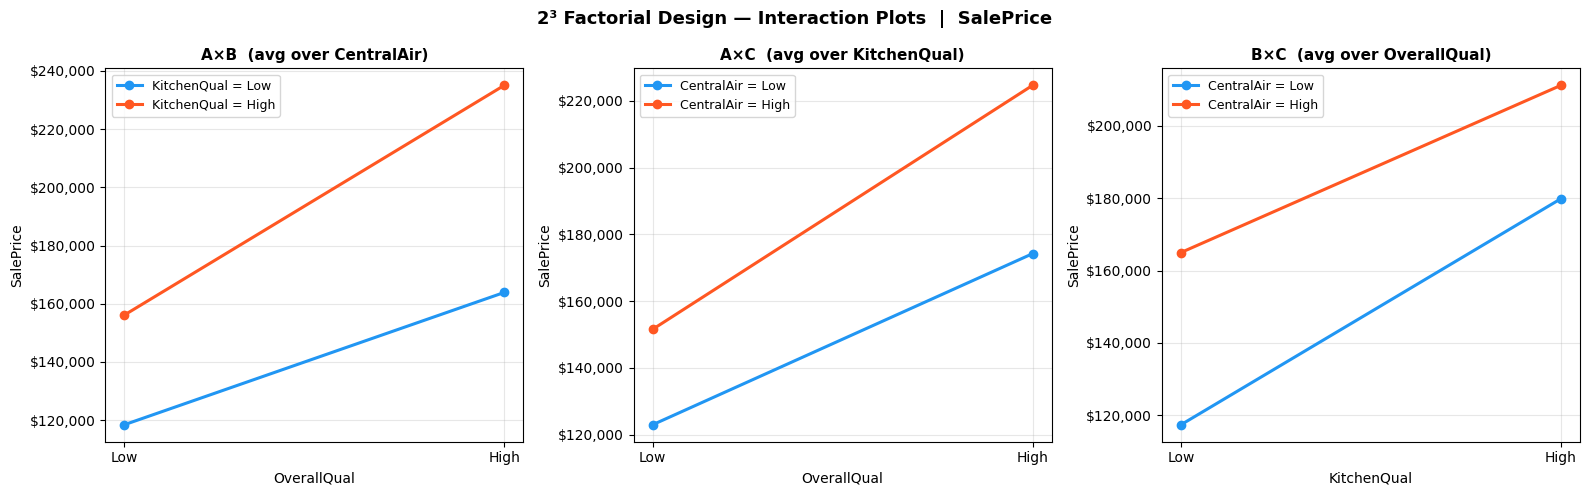
\includegraphics{figures/interaction_plots_saleprice.png}
\caption{Interaction plots SalePrice}
\end{figure}

\begin{figure}
\centering
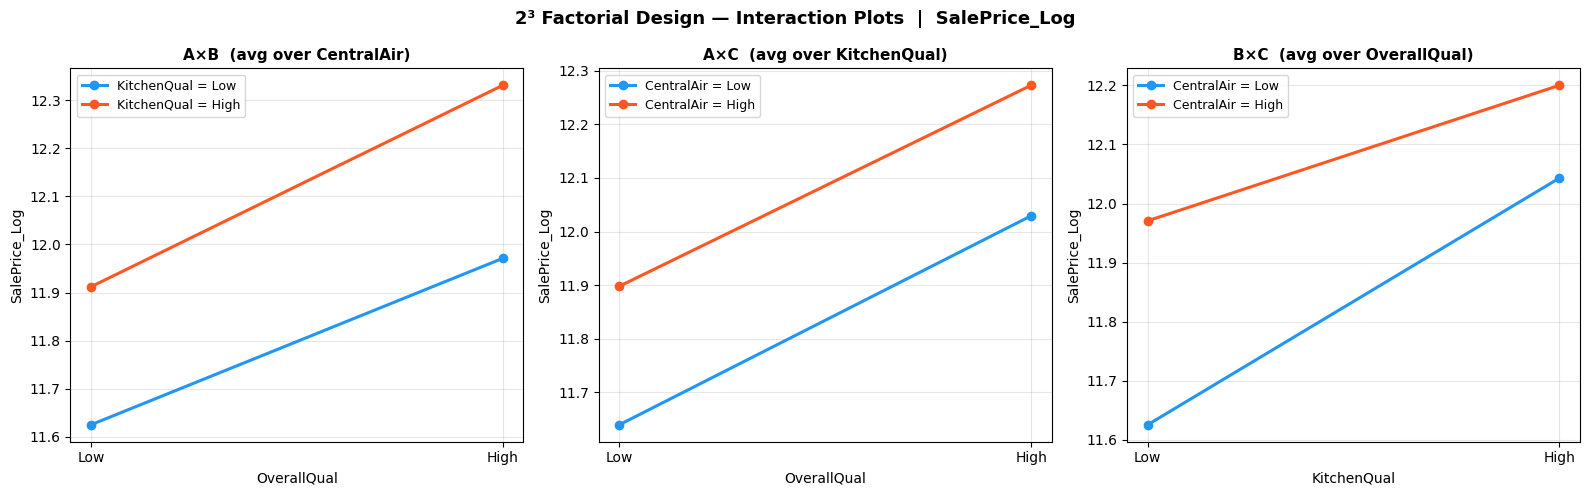
\includegraphics{figures/interaction_plots_log.png}
\caption{Interaction plots SalePrice\_Log}
\end{figure}

\begin{figure}
\centering
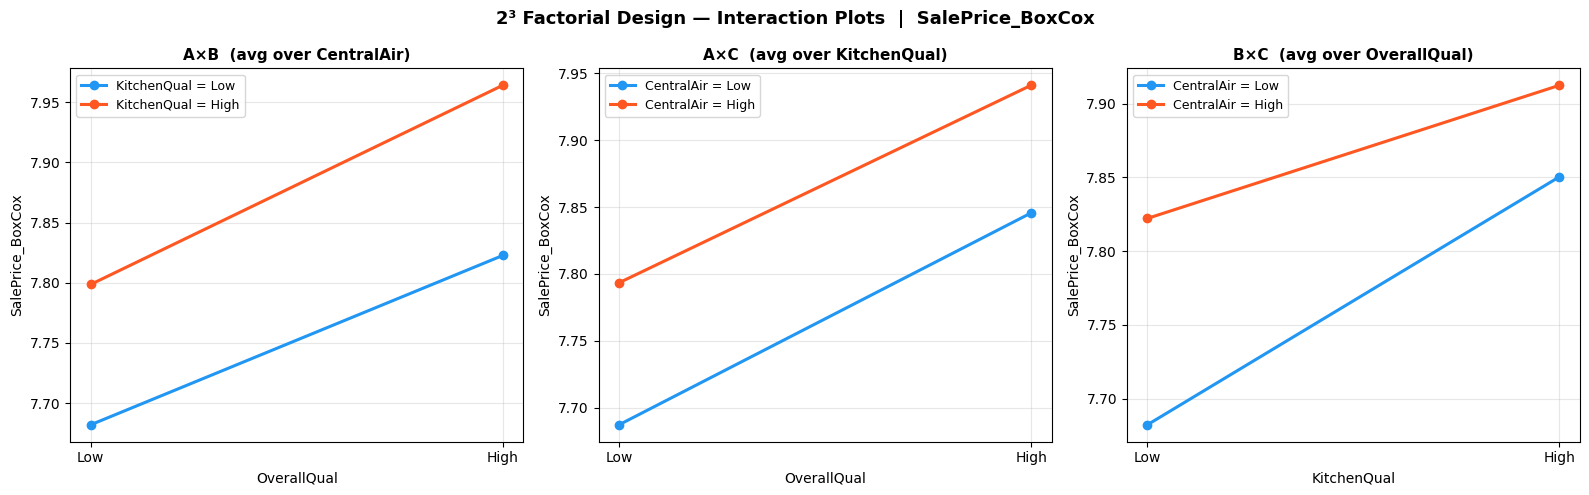
\includegraphics{figures/interaction_plots_boxcox.png}
\caption{Interaction plots SalePrice\_BoxCox}
\end{figure}

\emph{Figure 11: Interaction plots for the \(2^3\) factorial design on
the three target scales (top: \texttt{SalePrice}; middle:
\texttt{SalePrice\_Log}; bottom: \texttt{SalePrice\_BoxCox}). Each row
shows the three two-way interactions \(A \times B\), \(A \times C\), and
\(B \times C\), averaged over the third factor.}

Reading these plots: \textbf{parallel lines} mean no interaction (the
gap between the two levels of the modulating factor is constant);
\textbf{diverging or converging lines} mean a moderate interaction (the
gap grows or shrinks); \textbf{crossing lines} mean a strong interaction
with sign reversal. The slope of the lines reflects the main effect of
the primary factor; the gap between the lines reflects the main effect
of the modulating factor; the change in gap reflects the interaction.

\textbf{A × B (averaged over \texttt{CentralAir}).} On
\texttt{SalePrice}, the two lines (\texttt{KitchenQual\ =\ Low} in blue,
\texttt{KitchenQual\ =\ High} in red) both slope strongly upward but
\textbf{diverge} as \texttt{OverallQual} moves from Low to High. The gap
grows from roughly \$37k at Low to \$72k at High --- the two quality
factors amplify each other (a kitchen upgrade is worth more on a
high-quality house). This visual divergence corresponds to
\(A \times B = +\$16{,}740\), the largest two-way interaction on the
original scale. On \texttt{SalePrice\_Log} the divergence is much less
pronounced (the lines stay nearly parallel), matching
\(A \times B = +0.0365\) (\(+3.7\%\)). On \texttt{SalePrice\_BoxCox} the
lines look essentially parallel (\(A \times B = +0.0124\)). The pattern
is consistent in direction across the three scales (always positive) but
its magnitude shrinks dramatically under transformation --- a hallmark
of a \textbf{multiplicative effect} that becomes nearly additive after
the log transformation.

\textbf{A × C (averaged over \texttt{KitchenQual}).} On
\texttt{SalePrice}, the two lines both slope upward with the red line
slightly steeper, giving \(A \times C = +\$10{,}925\). On
\texttt{SalePrice\_Log} the two lines appear essentially parallel,
matching \(A \times C = -0.0074\) (\(-0.7\%\)) --- effectively zero. The
Box-Cox scale tells the same story (\(A \times C = -0.0054\)). The
visual reading confirms that \(A \times C\) is the weakest of the three
two-way interactions: the price gain from overall quality is roughly the
same whether the house has central air or not. The slight positive value
on the original scale is the only noticeable signal, and it disappears
on the transformed scales.

\textbf{B × C (averaged over \texttt{OverallQual}).} On
\texttt{SalePrice}, the two lines \textbf{converge} as
\texttt{KitchenQual} moves from Low to High. The blue line is steeper
than the red one: a kitchen upgrade adds more value to a house without
central air (\$62k jump) than to a house with central air (\$46k jump).
This convergence corresponds to \(B \times C = -\$8{,}140\), the only
\textbf{negative} two-way interaction. On \texttt{SalePrice\_Log} the
convergence is very visible --- the blue line ends higher than expected,
narrowing the gap significantly at \texttt{KitchenQual\ =\ High}. The
estimate is \(B \times C = -0.0941\) (\(-9.9\%\)), a substantial
negative interaction. Same pattern on Box-Cox
(\(B \times C = -0.0389\)). The economic reading: kitchen quality and
central air act as \textbf{partial substitutes} --- when one is present,
the marginal value of the other decreases.

\paragraph{Effect magnitude bar
charts}\label{effect-magnitude-bar-charts}

\begin{figure}
\centering
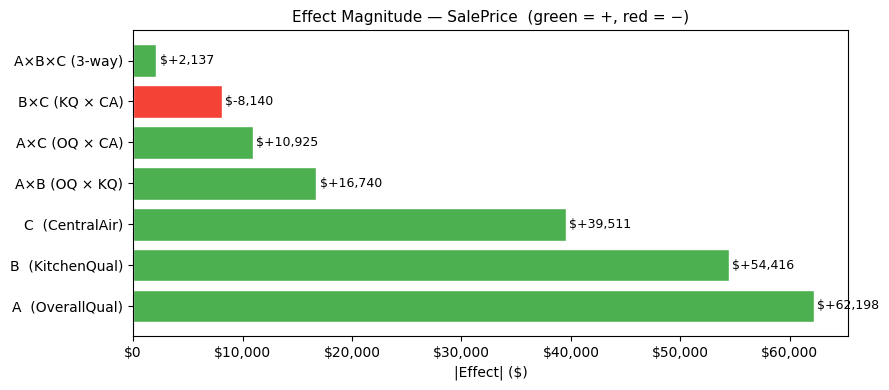
\includegraphics{figures/effect_bars_saleprice.png}
\caption{Effect bars SalePrice}
\end{figure}

\emph{(a) SalePrice}

\begin{figure}
\centering
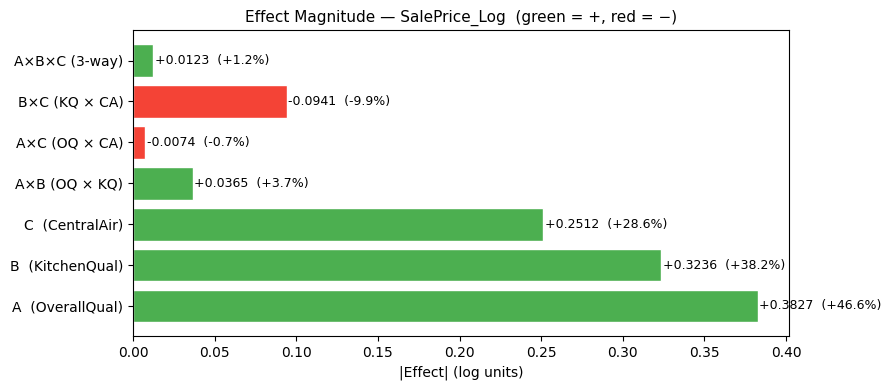
\includegraphics{figures/effect_bars_log.png}
\caption{Effect bars SalePrice\_Log}
\end{figure}

\emph{(b) SalePrice\_Log}

\begin{figure}
\centering
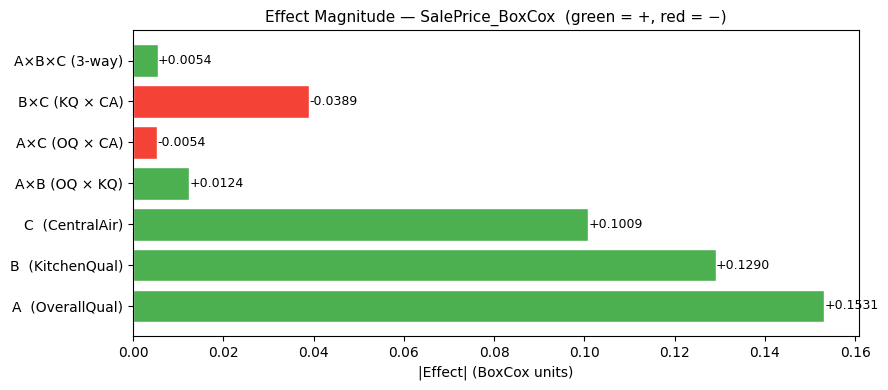
\includegraphics{figures/effect_bars_boxcox.png}
\caption{Effect bars SalePrice\_BoxCox}
\end{figure}

\emph{(c) SalePrice\_BoxCox}

\emph{Figure 12: Effect magnitude bar charts per target. Green bars:
positive effects (the High level increases price). Red bars: negative
effects. The three main effects (A, B, C) dominate by an order of
magnitude on every scale.}

\paragraph{Three-way interaction}\label{three-way-interaction}

The three-way interaction is \textbf{negligible on every target}:
\(+\$2{,}137\) on Original, \(+0.0123\) (\(+1.2\%\)) on Log, \(+0.0054\)
on Box-Cox. In all three cases, the magnitude is an order of magnitude
smaller than any two-way interaction and two orders smaller than any
main effect. This means the two-way interactions \emph{do not
meaningfully change} depending on the level of the third factor --- the
``average over the third factor'' approach used to compute them is fully
justified. The price structure can therefore be summarised by the main
effects and the two-way interactions, without needing to track
higher-order coupling.

\paragraph{Comparative interpretation across the three
targets}\label{comparative-interpretation-across-the-three-targets}

\textbf{The main effects ranking is identical and stable.} \(A > B > C\)
on every scale. The transformations change the magnitudes (dollars to
log units to Box-Cox units) but never the order. This is the strongest
signal of the analysis: the three factors carry genuine, scale-invariant
influence on price.

\textbf{Interactions are systematically smaller on the transformed
scales.} Compare \(A \times B\): \(+\$16{,}740\) (about 9\% of A's main
effect) on Original, but only \(+3.7\%\) on Log and \(+0.0124\) on
Box-Cox. Same compression for \(A \times C\) and
\(A \times B \times C\). The mechanism is well known: a transformation
that compresses the right tail of \texttt{SalePrice} also compresses the
multiplicative components of the data, which interactions encode. After
transformation, much of what appeared as ``interaction'' becomes
absorbed into additive main effects --- the transformations are
therefore not just useful for normality, they also reveal \textbf{how
additive the structure really is} once the scale is corrected.

\textbf{B × C is the most robust feature of the design.} It remains
negative on every target and visually clear in every interaction plot.
Unlike \(A \times B\) (where the magnitude shrinks under
transformation), \(B \times C\) even grows in relative importance on Log
(\(-9.9\%\) vs A's \(+46.6\%\) = roughly 21\% of A's effect, far larger
than its relative size on the original scale). This makes \(B \times C\)
the only interaction that should be carried forward as a structural fact
of the data --- not an artefact of scale.

\textbf{A × C is weak and unstable.} Positive on Original
(\(+\$10{,}925\)), nearly zero on Log (\(-0.7\%\)), nearly zero on
Box-Cox (\(-0.0054\)). Its direction even flips between Original and the
transformed scales, which is consistent with \(A \times C\) being
essentially absent from the price structure.

\paragraph{Operational verdict}\label{operational-verdict-1}

The \(2^3\) factorial design produces a clean, interpretable
decomposition of price into:

\begin{itemize}
\tightlist
\item
  \textbf{Three substantial and stable main effects:} A
  (\texttt{OverallQual}) \textgreater{} B (\texttt{KitchenQual})
  \textgreater{} C (\texttt{CentralAir}), each contributing a price
  premium in the tens of thousands of dollars range.
\item
  \textbf{One robust negative two-way interaction:} \(B \times C\),
  indicating that kitchen quality and central air act as partial
  substitutes in the price formation.
\item
  \textbf{One scale-dependent positive two-way interaction:}
  \(A \times B\), strong on the original scale but fading on the
  transformed scales --- likely a multiplicative effect that the
  transformations absorb.
\item
  \textbf{One negligible interaction:} \(A \times C\), near zero on
  every scale.
\item
  \textbf{No three-way coupling:} \(A \times B \times C\) is negligible
  everywhere.
\end{itemize}

The dominant message is that \textbf{the price structure is
overwhelmingly additive} in this binarised design, with one meaningful
interaction (\(B \times C\)) modulating the additive sum. The factorial
framework has successfully decomposed price into reusable building
blocks: a fixed baseline (the grand mean), three independent quality
premiums, and a single substitution effect between kitchen quality and
central air.

\begin{center}\rule{0.5\linewidth}{0.5pt}\end{center}

\subsection{6 Parametric Regression}\label{parametric-regression}

This section marks the transition from exploratory analysis (Sections
3--5) to predictive modelling. We build a parametric linear model ---
Ordinary Least Squares (OLS) --- using the features identified as
significant by ANOVA in Section 4, supplemented with two numerical
features capturing the size of the house. The model produces price
predictions as a linear combination of these inputs; we inspect its
coefficients, residual structure, and feature contributions before
comparing it to regularised alternatives (Ridge, Lasso).

\subsubsection{6.1 Model Specification}\label{model-specification}

\paragraph{Composition of the feature
set}\label{composition-of-the-feature-set}

We assemble 9 features for the regression:

\begin{itemize}
\tightlist
\item
  \textbf{7 ordinal quality features carried over from Section 4} ---
  \texttt{OverallQual}, \texttt{ExterQual}, \texttt{BsmtQual},
  \texttt{KitchenQual}, \texttt{FireplaceQu}, \texttt{CentralAir}, and
  \texttt{LotShape}. All seven were confirmed as significant drivers of
  price in the One-Way ANOVA of Section 4.2, so they form the natural
  categorical backbone of the model.
\item
  \textbf{2 numerical features prescribed by the assignment} ---
  \texttt{GrLivArea} (above-ground living area, in square feet) and
  \texttt{TotalBsmtSF} (total basement surface, in square feet). These
  introduce the \textbf{size} dimension of the house, which the 7
  quality features cannot capture on their own. Two houses with
  identical quality ratings can differ dramatically in price simply
  because one is twice the size of the other --- these two variables
  make that distinction available to the model.
\end{itemize}

The target variables are the usual three: \texttt{SalePrice},
\texttt{SalePrice\_Log}, \texttt{SalePrice\_BoxCox}.

\paragraph{Why ordinal encoding rather than
one-hot}\label{why-ordinal-encoding-rather-than-one-hot}

The 6 non-numerical features are \textbf{ordinal by nature}: there is a
meaningful order from ``worst'' to ``best'' (Po \textless{} Fa
\textless{} TA \textless{} Gd \textless{} Ex, or IR3 \textless{} IR2
\textless{} IR1 \textless{} Reg). We have two encoding choices:

\begin{itemize}
\tightlist
\item
  \textbf{One-hot encoding} would create a dummy column per level
  (e.g.~5 columns for \texttt{ExterQual}), turning each feature into a
  set of independent binary indicators. This discards the ordering
  information entirely --- the model would treat \texttt{Ex} and
  \texttt{Po} as no more related than two unrelated colours --- and it
  multiplies the number of columns from 9 to roughly 30, making
  interpretation heavier.
\item
  \textbf{Ordinal encoding} maps the levels to consecutive integers (Po
  → 1, \ldots, Ex → 5), preserving the order and keeping the feature set
  compact. The linear model can then estimate a single coefficient per
  feature representing how much price moves per quality step.
\end{itemize}

We adopt \textbf{ordinal encoding} because the ordering itself is the
primary signal carried by these features, and a parametric linear model
is built to exploit exactly this kind of monotonic relationship.

\paragraph{The equal-step assumption}\label{the-equal-step-assumption}

Ordinal encoding comes with a strong implicit assumption: by mapping Po
→ 1, Fa → 2, TA → 3, Gd → 4, Ex → 5, we tell the model that \textbf{the
gap between Po and Fa is exactly the same as the gap between Gd and Ex}.
In reality, the Tukey HSD tables in Section 4.3 already showed that
adjacent-level price gaps are highly uneven --- on \texttt{ExterQual}
for \texttt{SalePrice}, for example, Fa → TA is +\$56k, while TA → Gd is
+\$87k and Gd → Ex is +\$136k.

We accept this simplification as a deliberate trade-off: the equal-step
encoding is the price to pay for keeping the model linear,
interpretable, and compact. The residual diagnostics in Section 6.3 will
reveal whether the assumption causes systematic misfit.

\paragraph{The LotShape encoding --- an assumed
choice}\label{the-lotshape-encoding-an-assumed-choice}

The encoding IR3 → 1, IR2 → 2, IR1 → 3, Reg → 4 treats \texttt{LotShape}
as if it had a genuine ordinal scale running from ``most irregular'' to
``regular''. This is a defensible but \textbf{debatable} choice: in the
strict sense, IR1, IR2, IR3 describe degrees of irregularity but they do
not form a perfectly linear quality ladder, and Section 4 hinted that
the meaningful contrast might be \textbf{Regular vs Irregular} rather
than a continuous gradation among irregulars. We keep the ordinal
encoding here for uniformity with the other categorical features and let
the subsequent analysis (coefficient size, p-value, residual behaviour)
tell us whether this choice penalises the model.

\paragraph{Encoding pipeline and resulting
dataframe}\label{encoding-pipeline-and-resulting-dataframe}

The code follows a 4-step pipeline. Six features get explicit integer
mappings: the standard 5-level quality features (\texttt{ExterQual},
\texttt{KitchenQual}) follow \texttt{Po=1,\ Fa=2,\ TA=3,\ Gd=4,\ Ex=5};
the 6-level features with a \texttt{None} baseline (\texttt{BsmtQual},
\texttt{FireplaceQu}) follow \texttt{None=0,\ Po=1,\ ...,\ Ex=5};
\texttt{LotShape} follows \texttt{IR3=1,\ IR2=2,\ IR1=3,\ Reg=4};
\texttt{CentralAir} follows \texttt{N=0,\ Y=1}. \texttt{OverallQual} is
already integer-valued (1--10) and needs no mapping. The 9 features and
3 targets are then copied from \texttt{train} into a working dataframe
\texttt{df4}, with
\texttt{fillna(\textquotesingle{}None\textquotesingle{})} on the quality
columns so that missing entries are treated as the ``absence'' category.

A sanity check confirms the encoded ranges: \texttt{OverallQual} ∈ {[}1,
10{]}, \texttt{ExterQual} ∈ {[}2, 5{]}, \texttt{BsmtQual} ∈ {[}0, 5{]},
\texttt{KitchenQual} ∈ {[}2, 5{]}, \texttt{FireplaceQu} ∈ {[}0, 5{]},
\texttt{CentralAir} ∈ {[}0, 1{]}, \texttt{LotShape} ∈ {[}1, 4{]},
\texttt{GrLivArea} ∈ {[}334, 5642{]}, \texttt{TotalBsmtSF} ∈ {[}0,
6110{]}. Note that these encoding ranges differ substantially across
features, which has direct consequences for how raw coefficients should
be read --- a one-unit step on \texttt{OverallQual} (a 10-level scale)
is not the same operation as a one-unit step on \texttt{CentralAir} (a
2-level scale). We return to this point when interpreting the
coefficient tables below. The dataset has shape (1460, 12) with zero
missing values.

\subsubsection{6.2 Regression Results}\label{regression-results}

\paragraph{Overall fit quality}\label{overall-fit-quality}

We fit a separate OLS model on each of the three targets, using the 9
features without any interaction term. The summary statistics of the
three fits are:

\begin{longtable}[]{@{}lllll@{}}
\toprule\noalign{}
Target & R² & Adj. R² & F & p(F) \\
\midrule\noalign{}
\endhead
\bottomrule\noalign{}
\endlastfoot
\texttt{SalePrice} & 0.7786 & 0.7772 & 566.58 & ≈ 0 \\
\texttt{SalePrice\_Log} & 0.8159 & 0.8147 & 713.85 & ≈ 0 \\
\texttt{SalePrice\_BoxCox} & 0.8118 & 0.8106 & 694.83 & ≈ 0 \\
\end{longtable}

Three immediate observations:

\begin{itemize}
\tightlist
\item
  \textbf{The global F-test rejects \(H_0\) on every target}
  (\(p \approx 0\)), so the 9-feature model is globally meaningful on
  every scale.
\item
  \textbf{Transformed targets fit better.} \(R^2\) rises from 0.779 on
  the original scale to 0.816 on Log and 0.812 on Box-Cox, gaining
  roughly 4 percentage points. The same mechanism explored in Sections 3
  and 4 is at work: compressing the heavy right tail of
  \texttt{SalePrice} reduces the variance the linear model has to
  absorb, leaving a cleaner residual structure (as the diagnostics in
  Section 6.3 will confirm).
\item
  \textbf{The Log scale narrowly outperforms Box-Cox} (0.8159 vs
  0.8118), reversing the order observed in Section 3 where Box-Cox
  achieved the cleaner Shapiro--Wilk and skewness scores. This reversal
  is small (\(\Delta R^2 = 0.004\)) and consistent with the Box-Cox
  parameter being close to zero (\(\lambda \approx -0.0769\)); for
  predictive purposes, Log and Box-Cox should be treated as equivalent
  on this dataset, with Log slightly preferable because of its direct
  dollar interpretation via \texttt{np.expm1}.
\end{itemize}

\paragraph{Coefficient tables (raw, per-feature
units)}\label{coefficient-tables-raw-per-feature-units}

The tables below report the coefficient estimates, standard errors,
t-statistics, and p-values for the three OLS fits. The coefficients here
are reported \textbf{on the original feature scale} (one-unit increase
on each feature in its own encoding), not standardised.

\begin{longtable}[]{@{}lllll@{}}
\toprule\noalign{}
Feature & Coef & Std Err & t & p-value \\
\midrule\noalign{}
\endhead
\bottomrule\noalign{}
\endlastfoot
\texttt{OverallQual} & \$+14,989.4 & \$1,315.1 & 11.40 & 0.0000 *** \\
\texttt{ExterQual} & \$+16,116.3 & \$2,824.2 & 5.71 & 0.0000 *** \\
\texttt{BsmtQual} & \$+5,809.3 & \$1,593.4 & 3.65 & 0.0003 *** \\
\texttt{KitchenQual} & \$+16,098.0 & \$2,257.1 & 7.13 & 0.0000 *** \\
\texttt{FireplaceQu} & \$+3,145.4 & \$649.3 & 4.84 & 0.0000 *** \\
\texttt{CentralAir} & \$+8,678.9 & \$4,236.1 & 2.05 & 0.0407 * \\
\texttt{LotShape} & \$−6,448.9 & \$1,756.4 & −3.67 & 0.0002 *** \\
\texttt{GrLivArea} & \$+47.7 & \$2.5 & 19.12 & 0.0000 *** \\
\texttt{TotalBsmtSF} & \$+25.5 & \$2.9 & 8.69 & 0.0000 *** \\
\end{longtable}

\emph{Table 16: OLS coefficients on \texttt{SalePrice} (raw per-feature
units). Significance: *** p \textless{} 0.001, ** p \textless{} 0.01, *
p \textless{} 0.05, . p \textless{} 0.10.}

\begin{longtable}[]{@{}lllll@{}}
\toprule\noalign{}
Feature & Coef (log + \%) & Std Err & t & p-value \\
\midrule\noalign{}
\endhead
\bottomrule\noalign{}
\endlastfoot
\texttt{OverallQual} & +0.0883 (+9.2\%) & 0.0060 & 14.64 & 0.0000 *** \\
\texttt{ExterQual} & +0.0491 (+5.0\%) & 0.0130 & 3.79 & 0.0002 *** \\
\texttt{BsmtQual} & +0.0402 (+4.1\%) & 0.0073 & 5.51 & 0.0000 *** \\
\texttt{KitchenQual} & +0.0739 (+7.7\%) & 0.0104 & 7.14 & 0.0000 *** \\
\texttt{FireplaceQu} & +0.0199 (+2.0\%) & 0.0030 & 6.67 & 0.0000 *** \\
\texttt{CentralAir} & +0.2020 (+22.4\%) & 0.0194 & 10.40 & 0.0000 *** \\
\texttt{LotShape} & −0.0412 (−4.2\%) & 0.0081 & −5.11 & 0.0000 *** \\
\texttt{GrLivArea} & +0.0002 (+0.0\%) & 0.0000 & 19.40 & 0.0000 *** \\
\texttt{TotalBsmtSF} & +0.0001 (+0.0\%) & 0.0000 & 7.42 & 0.0000 *** \\
\end{longtable}

\emph{Table 17: OLS coefficients on \texttt{SalePrice\_Log} (raw
per-feature units). The ``\%'' annotation gives the percentage
equivalent \(e^\beta - 1\) per unit increase in the feature.}

\begin{longtable}[]{@{}lllll@{}}
\toprule\noalign{}
Feature & Coef & Std Err & t & p-value \\
\midrule\noalign{}
\endhead
\bottomrule\noalign{}
\endlastfoot
\texttt{OverallQual} & +0.0353 & 0.0024 & 14.60 & 0.0000 *** \\
\texttt{ExterQual} & +0.0181 & 0.0052 & 3.49 & 0.0005 *** \\
\texttt{BsmtQual} & +0.0161 & 0.0029 & 5.49 & 0.0000 *** \\
\texttt{KitchenQual} & +0.0288 & 0.0041 & 6.94 & 0.0000 *** \\
\texttt{FireplaceQu} & +0.0079 & 0.0012 & 6.60 & 0.0000 *** \\
\texttt{CentralAir} & +0.0858 & 0.0078 & 11.02 & 0.0000 *** \\
\texttt{LotShape} & −0.0164 & 0.0032 & −5.08 & 0.0000 *** \\
\texttt{GrLivArea} & +0.0001 & 0.0000 & 19.02 & 0.0000 *** \\
\texttt{TotalBsmtSF} & +0.0000 & 0.0000 & 7.18 & 0.0000 *** \\
\end{longtable}

\emph{Table 18: OLS coefficients on \texttt{SalePrice\_BoxCox} (raw
per-feature units).}

\paragraph{Interpretation of the
coefficients}\label{interpretation-of-the-coefficients}

\textbf{Every feature is statistically significant.} All 9 coefficients
have \(p < 0.05\) on all three targets, and 8 of the 9 are below
\(p < 0.001\). The only marginally significant case is
\texttt{CentralAir} on the original scale (\(p = 0.041\), three orders
of magnitude weaker than its significance on Log and Box-Cox, where
\(p < 10^{-23}\)). This is the first signal that \texttt{CentralAir} is
much more visible to the model once the price scale is normalised ---
the \(\eta^2\) analysis below quantifies this further.

\textbf{The dollar interpretation on \texttt{SalePrice} reads directly,
but per-step coefficients are not directly comparable.} Each unit
increase in an ordinal feature translates into an absolute dollar
amount: a one-step jump on \texttt{KitchenQual} (e.g.~from \texttt{TA}
to \texttt{Gd}) corresponds to +\$16,098, a one-step jump on
\texttt{OverallQual} corresponds to +\$14,989, and a one-step jump on
\texttt{ExterQual} corresponds to +\$16,116. An additional square foot
of living area contributes +\$47.7 and an additional square foot of
basement contributes +\$25.5 --- a coherent ranking where above-ground
living space is worth roughly twice basement space per square foot.

However, a per-step coefficient is \textbf{not an indicator of overall
importance}, because the features do not share the same encoding range.
\texttt{OverallQual} runs over 10 levels (1--10), \texttt{ExterQual}
over 4 observed levels (2--5), \texttt{CentralAir} over 2 levels (0--1),
and \texttt{GrLivArea} over thousands of square feet (334--5,642). A
feature with a smaller per-unit coefficient but a much wider range can
still dominate the total predicted variance --- which is precisely the
case for \texttt{GrLivArea}, as the \(\eta^2\) table below makes clear.
The standardised-coefficient table in Section 6.2 (Ridge/Lasso
comparison) re-expresses every coefficient as ``effect per one standard
deviation of the feature'', which is the unit needed to compare
contributions across features.

\textbf{The log scale exposes a counter-intuitive ranking.} On
\texttt{SalePrice\_Log}, the largest coefficient by magnitude is
\texttt{CentralAir} at +0.2020, equivalent to a +22.4\% price premium
for a binary jump. This is far larger in relative terms than the
per-unit effect of any quality variable (\texttt{OverallQual}
contributes only +9.2\% per step). The reason this was invisible on the
original scale is that the \texttt{CentralAir} contrast is binary --- a
single 0 → 1 jump cannot accumulate dollar magnitude the way a
multi-step ordinal can --- so its dollar coefficient looks small. The
log transformation expresses every coefficient as a \textbf{relative
price change}, which makes the binary jump directly comparable to the
per-step quality jumps, and the comparison clearly favours
\texttt{CentralAir}.

\textbf{The \texttt{LotShape} coefficient is negative on every target.}
The values are
−\(6,449 (Original), −0.0412 (Log, −4.2%), and −0.0164 (Box-Cox), all highly significant (
\)p \textless{} 0.001\$). Given the chosen encoding direction (1 = very
irregular, 4 = regular), \textbf{the negative sign means the model
predicts a slightly lower price as the lot becomes more regular, all
else equal.} This contradicts the intuitive expectation that regular
lots should command a premium. Two non-exclusive explanations are
consistent with the rest of the project:

\begin{itemize}
\tightlist
\item
  \textbf{The equal-step assumption is misfitting \texttt{LotShape}.}
  The Tukey analysis in Section 4.3 already established that the four
  levels do not form a clean monotonic ladder --- the three irregular
  levels were merged into one indistinguishable cluster on the
  transformed scales, while \texttt{Reg} stayed separate. Forcing a
  linear coefficient on a non-linear contrast can produce a sign that
  does not reflect the true marginal effect.
\item
  \textbf{Confounding with \texttt{GrLivArea}.} Larger and higher-end
  properties are sometimes built on irregular lots (corner plots,
  oversized irregular parcels, premium suburban developments). Once
  \texttt{GrLivArea} is controlled for, the residual effect of
  regularity may be negative because regularity correlates with smaller,
  denser-suburb properties.
\end{itemize}

The \(\eta^2\) ranking below will show that \texttt{LotShape} carries
very little explained variance regardless of its sign, so the
interpretation is informative but not decisive for predictive
performance.

\paragraph{ANOVA Type II --- which features explain the most
variance}\label{anova-type-ii-which-features-explain-the-most-variance}

The coefficients tell us \textbf{how} each feature shifts the
prediction, but not \textbf{how much} variance it explains. We run an
ANOVA Type II on each fitted model to decompose the total Sum of Squares
per feature. The choice of Type II is the same as in Section 4.3: it
tests each effect after accounting for all other effects simultaneously,
which is the correct option for an unbalanced design where features may
share information. The table below consolidates the F-statistics and
\(\eta^2\) values across the three targets.

\begin{longtable}[]{@{}
  >{\raggedright\arraybackslash}p{(\columnwidth - 12\tabcolsep) * \real{0.1429}}
  >{\raggedright\arraybackslash}p{(\columnwidth - 12\tabcolsep) * \real{0.1429}}
  >{\raggedright\arraybackslash}p{(\columnwidth - 12\tabcolsep) * \real{0.1429}}
  >{\raggedright\arraybackslash}p{(\columnwidth - 12\tabcolsep) * \real{0.1429}}
  >{\raggedright\arraybackslash}p{(\columnwidth - 12\tabcolsep) * \real{0.1429}}
  >{\raggedright\arraybackslash}p{(\columnwidth - 12\tabcolsep) * \real{0.1429}}
  >{\raggedright\arraybackslash}p{(\columnwidth - 12\tabcolsep) * \real{0.1429}}@{}}
\toprule\noalign{}
\begin{minipage}[b]{\linewidth}\raggedright
Feature
\end{minipage} & \begin{minipage}[b]{\linewidth}\raggedright
F (Orig.)
\end{minipage} & \begin{minipage}[b]{\linewidth}\raggedright
η² (Orig.)
\end{minipage} & \begin{minipage}[b]{\linewidth}\raggedright
F (Log)
\end{minipage} & \begin{minipage}[b]{\linewidth}\raggedright
η² (Log)
\end{minipage} & \begin{minipage}[b]{\linewidth}\raggedright
F (BC)
\end{minipage} & \begin{minipage}[b]{\linewidth}\raggedright
η² (BC)
\end{minipage} \\
\midrule\noalign{}
\endhead
\bottomrule\noalign{}
\endlastfoot
\texttt{GrLivArea} & 365.62 & 0.5158 & 376.26 & 0.4089 & 361.68 &
0.3983 \\
\texttt{OverallQual} & 129.92 & 0.1833 & 214.34 & 0.2329 & 213.27 &
0.2349 \\
\texttt{TotalBsmtSF} & 75.45 & 0.1064 & 55.11 & 0.0599 & 51.59 &
0.0568 \\
\texttt{KitchenQual} & 50.87 & 0.0718 & 51.01 & 0.0554 & 48.21 &
0.0531 \\
\texttt{ExterQual} & 32.56 & 0.0459 & 14.38 & 0.0156 & 12.21 & 0.0134 \\
\texttt{FireplaceQu} & 23.47 & 0.0331 & 44.48 & 0.0483 & 43.58 &
0.0480 \\
\texttt{LotShape} & 13.48 & 0.0190 & 26.12 & 0.0284 & 25.81 & 0.0284 \\
\texttt{BsmtQual} & 13.29 & 0.0188 & 30.31 & 0.0329 & 30.13 & 0.0332 \\
\texttt{CentralAir} & 4.20 & 0.0059 & 108.17 & 0.1176 & 121.49 &
0.1338 \\
\end{longtable}

\emph{Table 19: F-statistics and share of explained variance
(\(\eta^2\)) per feature from the Type II ANOVA decomposition. All
p-values are below 0.05, so every estimate is statistically supported.}

\textbf{\texttt{GrLivArea} dominates by a wide margin.} Living area
alone carries \textbf{51.6\% of the explained variance on the original
scale} and roughly 40\% on the transformed scales, with an F-statistic
of 365 on Original (a factor 2.8 above the second-ranked feature). The
two numerical size variables (\texttt{GrLivArea} + \texttt{TotalBsmtSF})
together account for \(\eta^2 = 0.62\) on the original scale, leaving
the 7 quality features collectively responsible for only the remaining
0.16. The implication is clear: \textbf{size, not quality, is the
dominant explanatory dimension} for an Ames house price. This validates
the assignment's choice to require these two numerical features
alongside the quality backbone --- without them the model would be
missing the principal axis of variation.

\textbf{\texttt{CentralAir} undergoes a spectacular rank change under
transformation.} On the original scale it contributes only \(F = 4.20\)
and \(\eta^2 = 0.0059\) (the weakest of all 9 features); on Log and
Box-Cox the F-statistic jumps to 108.17 and 121.49 respectively ---
\textbf{a factor 26--29 increase} that elevates \texttt{CentralAir} to
the third-largest contributor on the transformed scales
(\(\eta^2 = 0.118\) and 0.134). This mirrors the coefficient observation
above. The mechanism is the one observed throughout the project: the
heavy right tail of \texttt{SalePrice} inflates within-group variance
and drowns the binary \texttt{CentralAir} signal under noise on the
original scale; once the scale is normalised, the contrast --- which is
large in relative terms --- can dominate. \textbf{The transformation
does not change the underlying physical effect of central air on price;
it changes our ability to measure it cleanly.}

\textbf{The ranking of quality features is broadly stable.}
\texttt{OverallQual} is second on every target, \texttt{KitchenQual}
stays near the top of the quality features, and \texttt{LotShape} stays
near the bottom. \texttt{ExterQual} loses ground under transformation
(\(\eta^2\): 0.046 → 0.016, \(F\): 32.6 → 14.4), which is interesting
given that it was the strongest one-way F-statistic in Section 4.2
(\(F \approx 443\)). The interpretation is that \texttt{ExterQual} is
highly correlated with the other quality features and with
\texttt{OverallQual} in particular, so once those are in the model, its
unique contribution (which is what Type II measures) becomes modest.

\paragraph{Comparison with regularised regression (Ridge and
Lasso)}\label{comparison-with-regularised-regression-ridge-and-lasso}

To verify whether the OLS coefficients are stable and whether any
feature could be dropped without performance loss, we fit Ridge and
Lasso models on \textbf{standardised features} (\texttt{StandardScaler},
so every feature has mean 0 and standard deviation 1) and compare with
OLS via 5-fold cross-validated \(R^2\). The optimal regularisation
strength \(\alpha\) is selected by cross-validation.

\textbf{Important reading note --- coefficients here are not the same as
in Tables 16--18.} The coefficients in this comparison are expressed in
\textbf{standardised units}: each \(\beta\) is the price change per one
standard deviation of the feature, not per one unit on its native
encoding. To make the OLS coefficients comparable to Ridge/Lasso (which
are estimated on standardised features), we rescale them by the feature
standard deviations
(\(\beta_j^{\text{std}} = \beta_j^{\text{raw}} \times \sigma_j\)). This
is why the OLS \texttt{OverallQual} coefficient on Original appears as
+\$20,723 here but as +\$14,989 in Table 16 --- the same model, two
different units. Standardised coefficients are the unit needed for
\textbf{ranking feature importance}; raw coefficients are the unit
needed for \textbf{predicting price given a feature value}.

\begin{longtable}[]{@{}lllll@{}}
\toprule\noalign{}
Target & Model & R² (train) & R² (CV) & Alpha \\
\midrule\noalign{}
\endhead
\bottomrule\noalign{}
\endlastfoot
\texttt{SalePrice} & OLS & 0.7786 & --- & --- \\
\texttt{SalePrice} & Ridge & 0.7778 & 0.7671 & 123.2847 \\
\texttt{SalePrice} & Lasso & 0.7784 & 0.7686 & 628.0291 \\
\texttt{SalePrice\_Log} & OLS & 0.8159 & --- & --- \\
\texttt{SalePrice\_Log} & Ridge & 0.8153 & 0.8047 & 89.0215 \\
\texttt{SalePrice\_Log} & Lasso & 0.8157 & 0.8054 & 0.0031 \\
\texttt{SalePrice\_BoxCox} & OLS & 0.8118 & --- & --- \\
\texttt{SalePrice\_BoxCox} & Ridge & 0.8112 & 0.8006 & 89.0215 \\
\texttt{SalePrice\_BoxCox} & Lasso & 0.8116 & 0.8015 & 0.0012 \\
\end{longtable}

\emph{Table 20: Training \(R^2\) and 5-fold cross-validated \(R^2\) for
OLS, Ridge, and Lasso on the three targets. Ridge and Lasso are fit on
standardised features.}

\textbf{OLS does not overfit.} The gap between training \(R^2\) and
cross-validated \(R^2\) is only about 0.01 on every target (0.7786 →
0.7671 for Ridge on \texttt{SalePrice}; 0.8159 → 0.8047 for Ridge on
Log). This is a very small generalisation gap, which is consistent with
the feature-to-observation ratio (9 features, 1460 observations) being
healthy. Regularisation is therefore not needed for variance reduction
--- the OLS estimates are already stable.

\textbf{Lasso retains all 9 features on every target.} No coefficient is
shrunk to exactly zero, which is the clean answer Lasso provides to the
question ``can any feature be dropped?''. The answer here is
\textbf{no}: every feature in the set carries genuinely independent
information, with no redundancy that variable selection could exploit.
This justifies, after the fact, the feature-engineering choices made in
Section 4 (keeping only the 7 ANOVA-significant ordinal features) and in
the assignment (adding the two size variables).

\textbf{Coefficient signs and rankings are identical across the three
methods.} The structural conclusions of the OLS analysis --- the
negative sign on \texttt{LotShape}, the dominance of \texttt{GrLivArea}
and \texttt{OverallQual} in standardised terms, the scale-dependent
prominence of \texttt{CentralAir} --- carry over unchanged to Ridge and
Lasso. Ridge slightly attenuates the largest coefficients
(e.g.~\texttt{OverallQual} from +\$20,723 in OLS-standardised to
+\$18,979 in Ridge on \texttt{SalePrice}), as expected from its \(L^2\)
shrinkage, but the qualitative picture is preserved.

\textbf{Conclusion of the regularised comparison.} OLS is the
appropriate choice for this problem: the feature set is well-calibrated,
the model does not overfit, and no regularisation-based pruning is
warranted. Ridge and Lasso confirm rather than replace the OLS analysis.

\subsubsection{6.3 Model Diagnostics}\label{model-diagnostics}

The previous subsection established that the model fits the data well in
aggregate (\(R^2 \approx 0.78\)--\(0.82\)). What it does not yet
establish is whether the OLS assumptions --- linearity,
homoscedasticity, normally distributed residuals --- actually hold. If
they fail, the \(R^2\) remains a valid measure of in-sample fit but the
standard errors, t-statistics, and confidence intervals reported above
become unreliable. We examine three diagnostic plots per target and
complement them with a formal Shapiro--Wilk test on the residuals.

\textbf{Note on what is being tested here.} The Shapiro--Wilk test was
already used in Section 3 to verify the normality of \texttt{SalePrice}
itself --- a property of the \textbf{marginal} distribution of the
target. The test we run now addresses a structurally different question:
whether the regression \textbf{residuals}
\(\varepsilon_i = y_i - \hat{y}_i\) are normally distributed --- a
property of the \textbf{conditional} distribution of \(Y | X\). A
non-normal target can produce normal residuals (if the model captures
the non-normality via the features) and vice versa. The normality of
residuals, not the normality of \(Y\), is what determines whether the
OLS p-values and confidence intervals in Tables 16--18 can be trusted at
face value.

\textbf{Diagnostic plots.} We examine three plots per target:

\begin{itemize}
\tightlist
\item
  \textbf{Residuals vs Fitted.} A horizontal cloud centred on zero
  indicates that the linear specification captures the systematic
  component. A funnel shape, a curve, or a trend signals misfit.
\item
  \textbf{Normal Q-Q plot.} The quantiles of the residuals are plotted
  against the theoretical normal quantiles. Alignment with the reference
  line indicates approximately normal residuals.
\item
  \textbf{Scale-Location.} Plots
  \(\sqrt{|\text{standardised residuals}|}\) against fitted values. A
  horizontal cloud confirms homoscedasticity; a rising or trending shape
  signals heteroscedasticity.
\end{itemize}

\begin{figure}
\centering
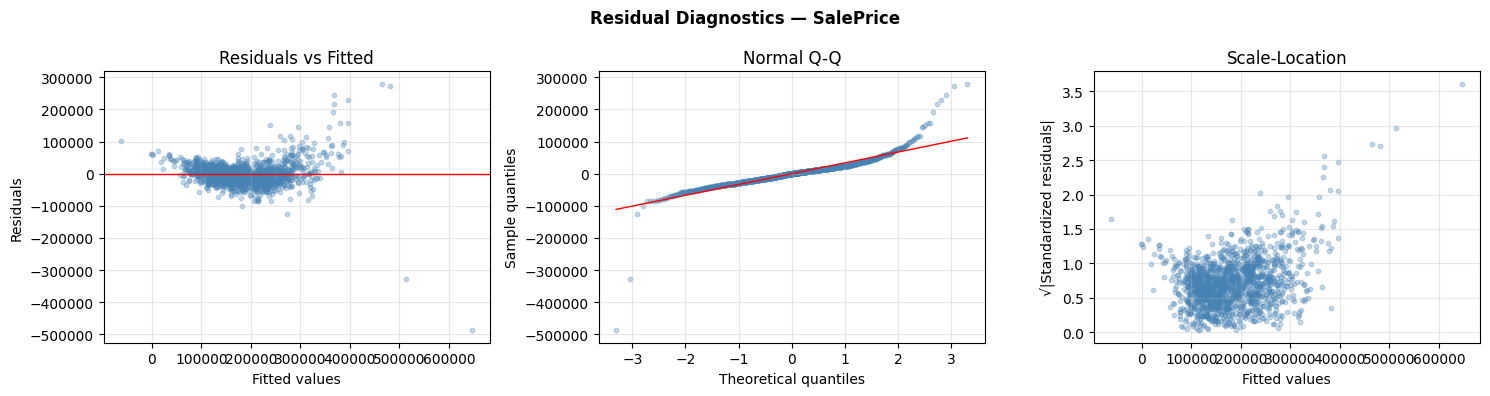
\includegraphics{figures/residual_diagnostics_saleprice.png}
\caption{Residual diagnostics SalePrice}
\end{figure}

\emph{SalePrice (original scale)}

\begin{figure}
\centering
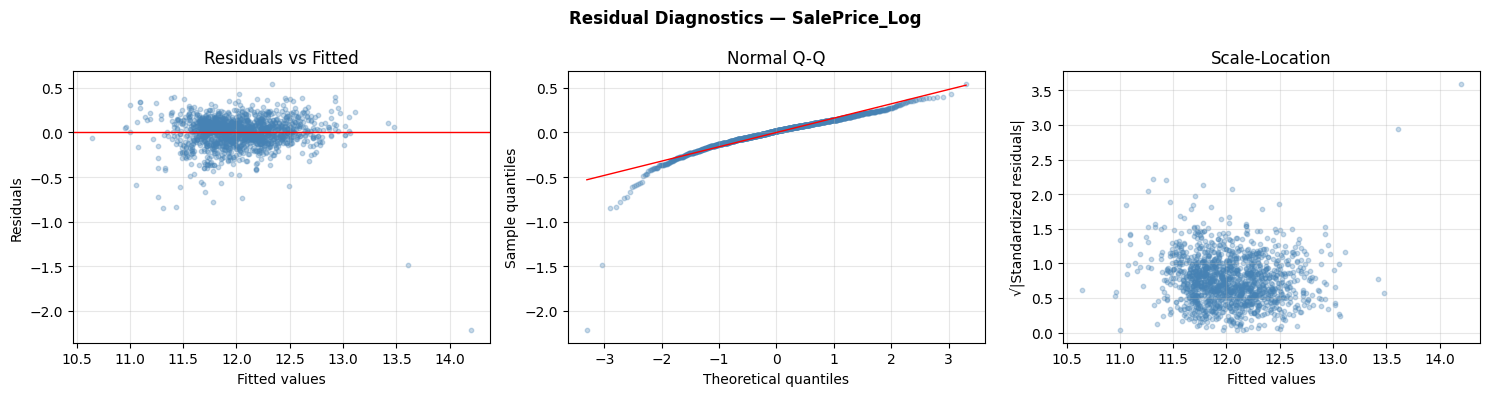
\includegraphics{figures/residual_diagnostics_log.png}
\caption{Residual diagnostics SalePrice\_Log}
\end{figure}

\emph{SalePrice\_Log}

\begin{figure}
\centering
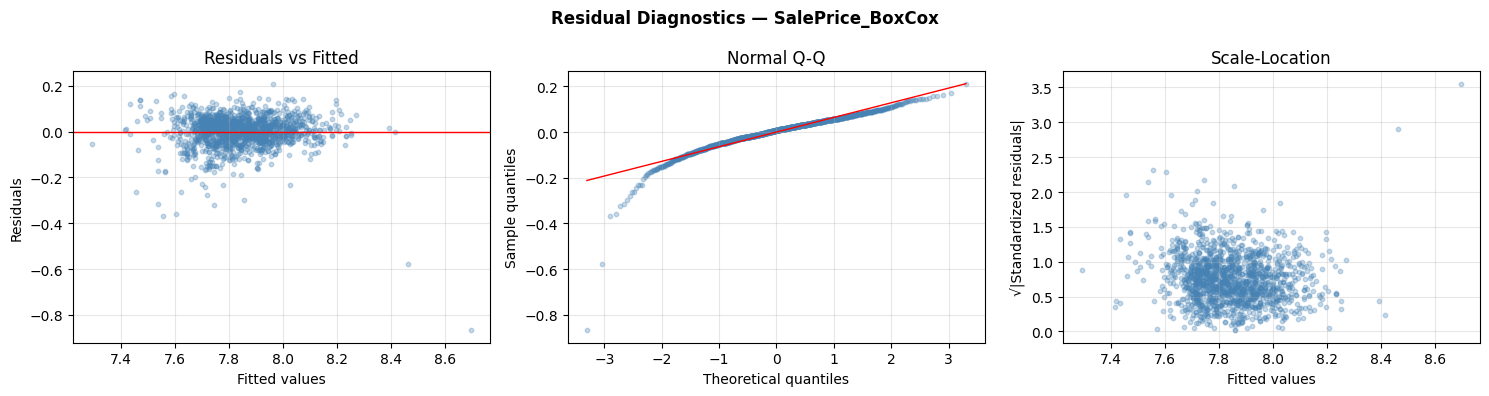
\includegraphics{figures/residual_diagnostics_boxcox.png}
\caption{Residual diagnostics SalePrice\_BoxCox}
\end{figure}

\emph{SalePrice\_BoxCox}

\emph{Figure 13: Residual diagnostics for the OLS model on each target.
Top: \texttt{SalePrice}; middle: \texttt{SalePrice\_Log}; bottom:
\texttt{SalePrice\_BoxCox}. For each target, from left to right:
Residuals vs Fitted, Normal Q-Q plot, and Scale-Location.}

\textbf{Shapiro--Wilk verdicts.} The formal test results on the
residuals of the three OLS fits are:

\begin{longtable}[]{@{}llll@{}}
\toprule\noalign{}
Target & W & p & Verdict \\
\midrule\noalign{}
\endhead
\bottomrule\noalign{}
\endlastfoot
\texttt{SalePrice} & 0.8117 & 3.05 × 10⁻³⁸ & non-normal × \\
\texttt{SalePrice\_Log} & 0.8753 & 1.22 × 10⁻³² & non-normal × \\
\texttt{SalePrice\_BoxCox} & 0.8711 & 4.52 × 10⁻³³ & non-normal × \\
\end{longtable}

The formal test \textbf{rejects normality on all three targets},
including Log and Box-Cox where the visual diagnostics looked
acceptable. We address the apparent contradiction below.

\textbf{On \texttt{SalePrice} (original scale) --- diagnostics fail
visually and formally.} The \textbf{Residuals vs Fitted} plot displays a
clear cone-shaped pattern: the spread of residuals is tight at low
fitted values (around ±\$30k for predictions of \$100k--\$200k) but
expands dramatically as fitted values grow (residuals of ±\$100k+ for
predictions of \$400k, and individual outliers reaching nearly −\$500k
at
\(650k). This is textbook **heteroscedasticity**: the variance of the errors is not constant but grows roughly proportionally with the predicted value. The **Normal Q-Q plot** confirms a heavy-tail problem in both directions: the upper-right tail rises sharply above the reference line, indicating a small number of houses whose actual price is much higher than the model predicts; the lower-left tail drops below the line, indicating houses whose actual price is much lower. The **Scale-Location plot** repeats the heteroscedasticity verdict from a different angle: the cloud trends upward as fitted values grow. The Shapiro–Wilk verdict (\)W
= 0.81\$, \(p \approx 10^{-38}\)) confirms the visual reading.

\textbf{On \texttt{SalePrice\_Log} --- diagnostics visually clean,
formal test still rejects.} The \textbf{Residuals vs Fitted} plot is
dramatically improved: the cloud is centred on zero across the entire
range of fitted values (from \(\sim 10.5\) to \(\sim 13.5\) in log
units, i.e.~\$36k to \$725k in dollar terms), and the spread is largely
uniform. A small number of negative outliers (residuals around \(-1.5\)
to \(-2\) log units, i.e.~houses that sold for 75--85\% below the
model's prediction) remain visible at low fitted values but no longer
dominate the plot. The \textbf{Normal Q-Q plot} closely tracks the
reference line from theoretical quantile \(-2\) to \(+2\), which covers
about 95\% of the residual mass; deviation remains visible only in the
extreme lower tail. The \textbf{Scale-Location plot} shows a roughly
horizontal cloud, confirming that the heteroscedasticity observed on the
original scale is essentially resolved.

The \textbf{Shapiro--Wilk test, however, still rejects normality}
(\(W = 0.875\), \(p \approx 10^{-32}\)). The apparent contradiction with
the visual reading is real and worth examining. Two mechanisms are at
work. First, on \(N = 1460\) observations \textbf{the Shapiro--Wilk test
has very high statistical power}: it detects even small departures from
normality that are invisible to the eye --- here, the residual mass in
the extreme lower tail (the 10--20 distressed-sale outliers identified
in the Q-Q plot) is enough to push the p-value below any conventional
threshold, even though it represents about 1\% of the data. Second,
\textbf{OLS inference is robust to mild violations of residual normality
in the large-sample regime}: by the Central Limit Theorem applied to
coefficient estimators, the t-statistics in Tables 17--18 remain
approximately normally distributed even when the underlying residuals
are not strictly Gaussian, provided the residuals have finite variance
--- which they do here. In practice, this means the p-values can still
be interpreted at face value for the bulk of the residual distribution;
only inference on the extreme lower tail (the distressed-sale outliers)
is genuinely uncertain.

\textbf{On \texttt{SalePrice\_BoxCox} --- diagnostics match Log.} The
three plots tell the same story as on the Log target, with no meaningful
qualitative difference, and the Shapiro--Wilk verdict (\(W = 0.871\),
\(p \approx 10^{-33}\)) matches the Log result. This is expected: the
optimal Box-Cox \(\lambda \approx -0.0769\) is close to zero (the value
at which Box-Cox becomes a logarithm). For diagnostic purposes, Log and
Box-Cox are interchangeable here.

\paragraph{What the diagnostics tell us about the modelling
strategy}\label{what-the-diagnostics-tell-us-about-the-modelling-strategy}

Three actionable conclusions emerge from the residual analysis:

\begin{itemize}
\tightlist
\item
  \textbf{The transformations are not optional --- they are required.}
  The original-scale model produces formally significant coefficients
  (\(p < 0.001\) for 8 of 9 features) and an apparently respectable
  \(R^2 = 0.78\), but its residual structure violates the
  homoscedasticity assumption so clearly that the reported standard
  errors are biased downward. The transformed targets both fix the
  heteroscedasticity and produce a better fit (\(R^2 \approx 0.82\)).
  Reporting the original-scale model alone would have been misleading.
\item
  \textbf{The equal-step ordinal encoding does not cause visible
  systematic misfit on the transformed scales.} The Residuals vs Fitted
  plots on Log and Box-Cox show no curvature, no fanning, and no banding
  that would betray a non-linear relationship between an ordinal feature
  and the target. The deliberate simplification accepted in Section 6.1
  is therefore vindicated --- the model is not fighting the data.
\item
  \textbf{Residual normality is formally rejected on every scale, but
  does not undermine the inference on Log/Box-Cox.} The Shapiro--Wilk
  verdict on the transformed targets reflects the high power of the test
  on \(N = 1460\) and a small population of low-end outliers (about
  10--20 houses whose actual price is much lower than the model
  predicts). These outliers cannot be eliminated by a different choice
  of transformation --- they reflect a real phenomenon at the bottom of
  the housing market that the available features simply do not capture,
  and they are the same kind of cases the neural network in Section 7
  will encounter. For the bulk of the residual distribution, OLS
  inference on Log and Box-Cox remains usable thanks to the large-sample
  robustness of the t-tests.
\end{itemize}

\paragraph{Operational verdict}\label{operational-verdict-2}

The parametric regression analysis produces the following findings:

\begin{itemize}
\tightlist
\item
  \textbf{The model is globally significant on all three targets}, with
  \(R^2 = 0.78\) (Original), 0.82 (Log), 0.81 (Box-Cox). Every feature
  contributes a significant coefficient.
\item
  \textbf{The transformed targets are the appropriate scales for the
  linear model.} The original scale violates the homoscedasticity
  assumption catastrophically; the transformations restore it almost
  entirely, and large-sample robustness compensates for the residual
  normality the formal test still rejects.
\item
  \textbf{The dominant explanatory feature is \texttt{GrLivArea}}, with
  \(F = 365\) and \(\eta^2 = 0.52\) on the original scale --- by a
  factor 2.8 above the second-ranked feature. The 7 quality features
  collectively account for less than the two size variables, validating
  the assignment's choice of including \texttt{GrLivArea} and
  \texttt{TotalBsmtSF} alongside the ANOVA-significant ordinal backbone.
\item
  \textbf{\texttt{CentralAir} is the most scale-sensitive feature}, with
  its F-statistic increasing by a factor 26--29 between Original
  (\(F = 4.20\)) and Log/Box-Cox (\(F = 108\) and \(F = 121\)). This is
  consistent with the rest of the project: the heavy right tail of
  \texttt{SalePrice} masks effects that the transformed scales correctly
  expose.
\item
  \textbf{The model is stable and the feature set is well-calibrated.}
  Ridge and Lasso match OLS within 0.01 on cross-validated \(R^2\),
  Lasso retains every feature, and all three methods agree on signs and
  rankings when read in standardised units.
\item
  \textbf{The negative \texttt{LotShape} coefficient is real but minor.}
  It reflects either the imperfect equal-step encoding of an essentially
  non-monotonic feature, or confounding with size. The feature
  contributes little explained variance, so the interpretive ambiguity
  does not affect predictive performance.
\end{itemize}

This OLS model, with \(R^2 \approx 0.82\) on the transformed targets,
sets the parametric benchmark that the non-parametric neural network of
Section 7 will aim to surpass by exploiting the full 79-feature space
and non-linear interactions that OLS cannot represent.

\begin{center}\rule{0.5\linewidth}{0.5pt}\end{center}

\subsection{7 Neural-Network
Regression}\label{neural-network-regression}

This section marks a fundamental shift in methodology. Up to now, every
model and analysis assumed a specific functional form ---
\textbf{linearity} in OLS, \textbf{additivity} in ANOVA,
\textbf{equal-step distances} in ordinal encoding, predefined effect
contrasts in the factorial design. These assumptions made the analysis
interpretable but also imposed strong structural constraints on what the
data could tell us. A \textbf{Multi-Layer Perceptron (MLP)}, in
contrast, is a \textbf{non-parametric} model: it makes almost no
assumption about how features relate to the target and learns the
mapping directly from data through stacked non-linear transformations.

This section also produces the final \textbf{Kaggle submission} of the
project. The competition evaluates submissions using the Root Mean
Squared Error (RMSE) between the predicted and observed
\(\log(\text{SalePrice})\), so the metric itself operates on the log
scale, not on raw dollars. We therefore train the network on
\texttt{SalePrice\_Log} for two converging reasons: \textbf{alignment
with the Kaggle metric} (the loss we minimise is exactly the quantity
Kaggle judges), and \textbf{consistency with the analytical findings
from Sections 3--6} (the log transformation reduces skewness from 1.883
to 0.121, compresses outliers, stabilises variance across price ranges,
and makes feature effects more nearly additive --- all properties an MLP
benefits from). The final submission back-converts the predictions via
\texttt{np.expm1} to recover dollar amounts; the pair
\texttt{log1p}/\texttt{expm1} is mathematically exact, so no information
is lost in the round-trip.

\subsubsection{7.1 Model Inputs and
Preprocessing}\label{model-inputs-and-preprocessing}

\paragraph{Feature inspection}\label{feature-inspection}

Sections 4--6 worked on a hand-picked subset of 9 features (7 ordinal
qualities plus \texttt{GrLivArea} and \texttt{TotalBsmtSF}). This
section follows the assignment's mandate to leverage \textbf{all
available features}: we reload \texttt{train.csv} and \texttt{test.csv}
from scratch and keep every column except \texttt{Id} (no predictive
signal --- the test \texttt{Id}s are saved aside as \texttt{test\_ids}
for the submission file) and \texttt{SalePrice} (the target). The
resulting input space contains \textbf{79 features}: 36 numerical
(continuous quantities like \texttt{GrLivArea}, \texttt{LotArea},
\texttt{YearBuilt}, plus integer-coded ordinals like
\texttt{OverallQual}) and 43 categorical (text-valued attributes such as
\texttt{Neighborhood}, \texttt{HouseStyle}, and all the quality grades).
This is roughly 9× more raw input information than the linear model
used, at the cost of a substantial volume of missing values that must be
handled robustly.

The missing-value pattern splits into three regimes. \textbf{Massive
missingness with clear semantics} (``feature is genuinely absent''):
\texttt{PoolQC} 99.5\%, \texttt{MiscFeature} 96.3\%, \texttt{Alley}
93.8\%, \texttt{Fence} 80.8\%, \texttt{FireplaceQu} 47.3\%.
\textbf{Moderate missingness, also semantic}: \texttt{MasVnrType}
(59.7\%), the five \texttt{Garage*} features (\textasciitilde5.5\% each,
consistent across columns confirming a single mechanism --- no garage),
the five \texttt{Bsmt*} features (\textasciitilde2.5\% each, no
basement). \textbf{True missing data}, the only column where NaN
plausibly means ``this measurement is missing'' rather than ``the
feature is absent'': \texttt{LotFrontage} (17.7\% on train, 15.6\% on
test). The pattern is highly consistent between train and test --- no
surprise NaN columns appear in test that the pipeline would not have
seen during training.

The categorical cardinality profile is dominated by
\texttt{Neighborhood} (25 levels), \texttt{Exterior2nd} (16),
\texttt{Exterior1st} (15), followed by \texttt{Condition1},
\texttt{SaleType} (9 each) and a tail of features with 6--8 levels. The
43 categorical features sum to 251 distinct levels, which after one-hot
encoding will expand the feature space to a few hundred columns.

\paragraph{Preprocessing pipeline}\label{preprocessing-pipeline}

Three preprocessing operations must be applied in a strict order on a
neural-network feature set: \textbf{impute missing values, encode
categoricals, standardise numerics}. Doing these manually introduces two
recurring bugs --- inconsistency between train and test (forgetting to
apply the same medians and category mappings), and information leakage
(computing statistics on train and test combined). The
\texttt{sklearn.Pipeline\ +\ ColumnTransformer} pattern eliminates both
risks structurally: every transformation is \textbf{fit on train only},
and the fitted parameters are then transformed onto test.

\begin{itemize}
\tightlist
\item
  \textbf{Numerical pipeline (36 columns):}
  \texttt{SimpleImputer(strategy=\textquotesingle{}median\textquotesingle{})}
  → \texttt{StandardScaler}. Median imputation is robust to the
  heavy-tailed columns (\texttt{LotArea}, \texttt{GrLivArea});
  standardisation puts every feature on a common (mean 0, std 1)
  footing, which is critical for an MLP --- without scaling, features
  measured in thousands (\texttt{LotArea}) would dominate the gradient
  while features measured in single digits (\texttt{OverallQual}) would
  barely contribute.
\item
  \textbf{Categorical pipeline (43 columns):}
  \texttt{SimpleImputer(strategy=\textquotesingle{}constant\textquotesingle{},\ fill\_value=\textquotesingle{}Missing\textquotesingle{})}
  →
  \texttt{OneHotEncoder(handle\_unknown=\textquotesingle{}ignore\textquotesingle{},\ sparse\_output=False)}.
  The constant-string imputation preserves the semantic distinction
  between ``feature absent'' and the other levels rather than collapsing
  it into the most-frequent class. The
  \texttt{handle\_unknown=\textquotesingle{}ignore\textquotesingle{}}
  policy is a safety net at prediction time: if the test set contains a
  level absent from train, the affected row is encoded as a zero-vector
  across all known levels rather than crashing.
\end{itemize}

\paragraph{Unknown category detection in
test}\label{unknown-category-detection-in-test}

The \texttt{\textquotesingle{}ignore\textquotesingle{}} fallback is
silent by default --- the model would receive zero-vectors without us
knowing. To stay informed, we explicitly compare the test set's
categorical levels against the levels the encoder learned from train.
The audit detected \textbf{7 categorical features where test contains a
level absent from train}: \texttt{MSZoning} (4 rows), \texttt{Utilities}
(2), \texttt{Exterior1st} (1), \texttt{Exterior2nd} (1),
\texttt{KitchenQual} (1), \texttt{Functional} (2), \texttt{SaleType}
(1). In every case the unknown level is
\texttt{\textquotesingle{}Missing\textquotesingle{}} --- a known
asymmetry in the Kaggle House Prices dataset: these 7 columns have no
NaN in train but do have NaN in test. Our imputer faithfully labels them
\texttt{\textquotesingle{}Missing\textquotesingle{}} on both sides, but
because the level never appeared in train, the encoder never learned it.
The affected observations total at most \textbf{12 test rows out of 1459
(≈ 0.8\%)}, most with only one unknown column out of 43, so the rest of
each row's encoded vector is well-formed. We accept the zero-vector
fallback rather than injecting the
\texttt{\textquotesingle{}Missing\textquotesingle{}} level into train
artificially: the volume is negligible (impact on RMSE in the noise),
the semantics of a zero-vector are interpretable (``no positive evidence
for any known level''), and modifying the training set would break the
train/test separation.

\paragraph{Resulting input dimensions}\label{resulting-input-dimensions}

The 79 raw features expand to \textbf{303 numerical columns}: the 36
numerical features standardised in place, and the 43 categorical
features expanded into 267 one-hot columns (an average of 6.2 levels per
categorical feature). Train shape (1460, 303), test shape (1459, 303),
zero remaining NaN on either side. The 5:1 ratio of observations to
columns is comfortable for an MLP with L2 regularisation and early
stopping.

\subsubsection{7.2 Training and
Validation}\label{training-and-validation}

\paragraph{Baseline model}\label{baseline-model}

We first fit a baseline MLP to establish a reference point: architecture
\texttt{(128,\ 64)} (two hidden layers), ReLU activations, Adam
optimiser, \(\alpha = 10^{-3}\) (modest L2 regularisation),
\texttt{learning\_rate\_init=10\^{}\{-3\}}, early stopping with
\texttt{validation\_fraction=0.1} and \texttt{n\_iter\_no\_change=20}.
Evaluated on a single external 20\% validation split held out from
training, the baseline reaches \textbf{RMSE = 0.1724} and
\textbf{\(R^2 = 0.8407\)} on this validation split. The numbers are
taken at face value here but with one caveat: a single random split
gives a noisy estimate of generalisation performance, easily ±0.02 in
RMSE depending on which observations end up in the holdout. The tuning
step that follows replaces this single-split protocol with
cross-validation precisely to obtain a more reliable headline number.

\paragraph{Hyperparameter tuning via
GridSearchCV}\label{hyperparameter-tuning-via-gridsearchcv}

The baseline hyperparameters were sensible defaults, but not
data-justified. We search systematically over a compact grid of
\textbf{18 combinations}, focused on the three hyperparameters that
materially affect MLP performance: \texttt{hidden\_layer\_sizes} ∈
\{\texttt{(64,)}, \texttt{(128,\ 64)}, \texttt{(256,\ 128,\ 64)}\}
(shallow vs.~medium vs.~deep), \(\alpha\) ∈
\{\(10^{-4}, 10^{-3}, 10^{-2}\)\} (three orders of magnitude of
regularisation), and \texttt{learning\_rate\_init} ∈
\{\(10^{-3}, 5 \times 10^{-4}\)\}. All other hyperparameters
(activation, solver, early-stopping policy, random seed) are held
constant.

\textbf{Protocol --- 100\% of training data, no external split.} Step
3-bis abandons the 20\% external validation split and uses the
\textbf{entire training set} for both the hyperparameter search and the
final model fit. Three justifications: \textbf{data efficiency} (with
only 1460 observations, every row counts --- reserving 292 of them as an
untouched holdout means GridSearchCV evaluates each combination on a
smaller pool); \textbf{honesty preserved by cross-validation} (each
candidate is evaluated by 3-fold CV inside \texttt{GridSearchCV}, so
every hyperparameter score is averaged over 3 distinct held-out subsets
--- the CV RMSE is an honest estimate of out-of-sample performance); and
\textbf{final refit on 100\%} (once the best configuration is
identified, \texttt{GridSearchCV} automatically refits it on the full
training set via \texttt{refit=True}). The trade-off: we no longer have
a single fresh held-out number to compare against; instead, the CV RMSE
of the winning configuration is the most reliable estimate of
generalisation performance.

\textbf{Winning configuration.} The grid search identified
\texttt{hidden\_layer\_sizes=(64,)}, \texttt{alpha=10⁻²},
\texttt{learning\_rate\_init=10⁻³}, with a \textbf{best CV RMSE on log
scale of 0.1821}. The most striking finding is the architectural choice:
the winning model is the \textbf{shallowest and smallest option in the
grid} --- a single hidden layer of 64 neurons. Both \texttt{(128,\ 64)}
and \texttt{(256,\ 128,\ 64)} performed worse on cross-validation. This
is a clear signal that the dataset does not warrant a deep network: with
1460 observations and a feature space dominated by sparse one-hot
indicators (267 of 303 columns), additional capacity becomes
\textbf{noise capacity} rather than signal capacity. The strong
regularisation (\(\alpha = 10^{-2}\), the highest value tested)
reinforces this reading --- the optimum sits at the boundary of the grid
where shrinkage is most aggressive.

\textbf{Robustness --- top-5 analysis.} The five best configurations all
share the same architecture and differ only in \(\alpha\) and learning
rate:

\begin{longtable}[]{@{}llllll@{}}
\toprule\noalign{}
Rank & Architecture & α & lr & RMSE & Std \\
\midrule\noalign{}
\endhead
\bottomrule\noalign{}
\endlastfoot
1 & (64,) & 10⁻² & 10⁻³ & 0.1821 & 0.0264 \\
2 & (64,) & 10⁻³ & 10⁻³ & 0.1829 & 0.0265 \\
3 & (64,) & 10⁻⁴ & 10⁻³ & 0.1831 & 0.0266 \\
4 & (64,) & 10⁻² & 5×10⁻⁴ & 0.1852 & 0.0258 \\
5 & (64,) & 10⁻³ & 5×10⁻⁴ & 0.1858 & 0.0259 \\
\end{longtable}

Three readings emerge. The architectural choice \texttt{(64,)} is robust
--- every top-ranked candidate agrees on it. The exact value of
\(\alpha\) matters less than the architecture: RMSE varies by only 0.001
over three orders of magnitude. \texttt{learning\_rate\_init\ =\ 10⁻³}
consistently beats \texttt{5×10⁻⁴}. The high standard deviation across
CV folds (≈ 0.026) compared to the gap between candidates (≈ 0.001)
means the top 3 are practically equivalent and the winner could shift
between random seeds.

\textbf{Final model behaviour and baseline comparison.} After refitting
on the full training set, the tuned model stops at \textbf{304
iterations} out of 500 max (early stopping triggered cleanly), with
final training loss 0.006165 --- higher than the baseline's 0.002017,
which is expected and desirable: the higher loss reflects the stronger
regularisation, which trades a bit of training fit for better
generalisation. In-sample predictions reach \textbf{RMSE = 0.0884 log
units, \(R^2 = 0.9510\)} on the training set, MAE ≈ \$10,675, RMSE ≈
\$15,899 in dollars. These in-sample numbers are biased upward by
construction (the model has seen this data during training); the true
expected performance on unseen data is closer to the CV RMSE of 0.1821
--- about twice the in-sample value, a normal generalisation gap for a
regularised MLP on a dataset of this size.

At first glance the tuned model looks \textbf{worse} than the baseline
(RMSE 0.1821 vs.~0.1724). But the comparison is misleading: the baseline
number comes from a single random split that may have favoured the model
by luck, while the tuned number is an average over 3 folds, far more
reliable. The CV RMSE is the number we should trust for the Kaggle
expectation, and the tuned model is more principled --- every
hyperparameter is justified by the data rather than picked \emph{a
priori}.

\paragraph{Residual diagnostics on the tuned
MLP}\label{residual-diagnostics-on-the-tuned-mlp}

Before generating the Kaggle submission, we audit the structure of the
residuals. A model can achieve a low average RMSE while still exhibiting
systematic biases --- over-predicting cheap houses, under-predicting
luxury houses, producing variance that grows with the predicted value.
The diagnostics detect such patterns. One caveat: unlike Section 6 where
we had a clear in-sample / out-of-sample distinction, all residuals here
are computed in-sample (Protocol B). The diagnostics report on how well
the model fits the training data, not on how well it generalises --- the
honest estimate of generalisation performance remains the CV RMSE of
0.1821.

\begin{figure}
\centering
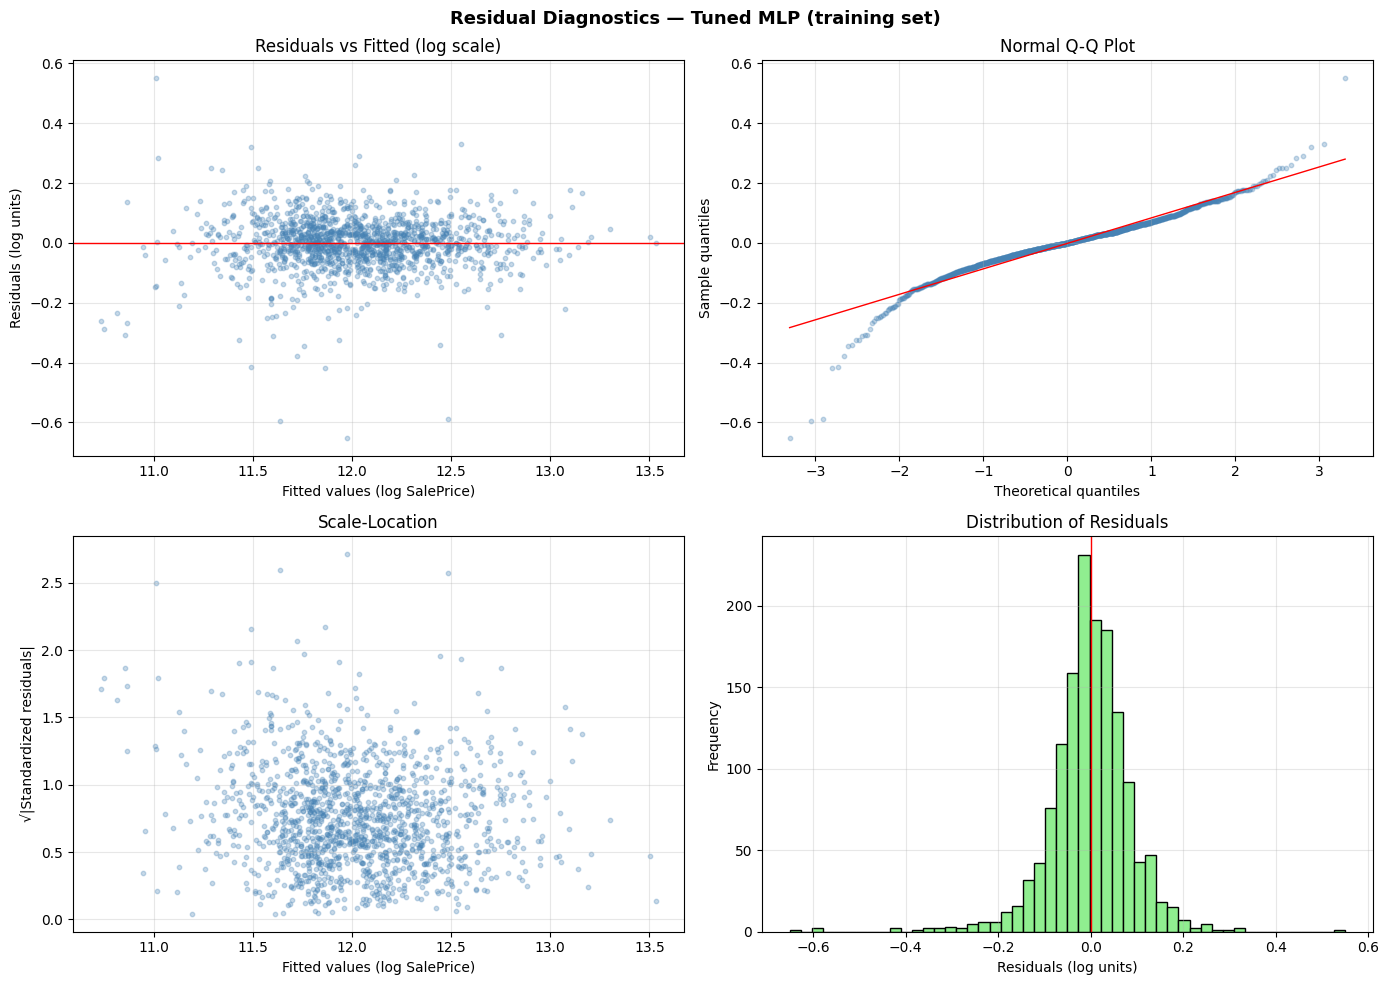
\includegraphics{figures/mlp_residual_diagnostics.png}
\caption{Residual diagnostics for the tuned MLP}
\end{figure}

\emph{Figure 14: Residual diagnostics for the tuned MLP on the training
set. Top-left: Residuals vs Fitted (log scale). Top-right: Normal Q-Q
plot. Bottom-left: Scale-Location. Bottom-right: Distribution of
Residuals.}

The numerical summary, with residuals defined as
\(y_{\text{true}} - y_{\text{pred}}\) in log units (so a
\textbf{negative residual indicates an over-prediction}):

\begin{longtable}[]{@{}llll@{}}
\toprule\noalign{}
Statistic & Value & Statistic & Value \\
\midrule\noalign{}
\endhead
\bottomrule\noalign{}
\endlastfoot
Mean & −0.001417 & Min & −0.651248 \\
Median & −0.000124 & Max & +0.550382 \\
Std & 0.088432 & Skewness & −0.844356 \\
Kurtosis (excess) & +7.107303 & Shapiro--Wilk W & 0.9284 \\
& & Shapiro--Wilk p & 7.76 × 10⁻²⁶ \\
\end{longtable}

\textbf{Residuals vs.~Fitted.} The cloud is \textbf{centred around zero}
across the full range of fitted values (≈ 10.7 to 13.5 on the log scale,
roughly \$45k to \$725k). No curve, slope, or trend appears --- the
model captures the systematic relationship between features and price
across the price spectrum. The cloud is slightly narrower in the middle
(fitted ≈ 11.5--12.5) and wider at the extremes, a faint signal the
Scale-Location plot will resolve. A few outliers stand out below the
cloud at low and middle fitted values, reaching residuals of −0.4 to
−0.65 (over-predictions of 33--90\%) --- these are the worst cases
identified below.

\textbf{Normal Q-Q plot.} The bulk of the residuals follows the
reference line closely --- the central ≈ 80\% of the distribution is
nearly normal. The \textbf{lower tail (theoretical quantile \textless{}
−2) deviates sharply downward}, indicating residuals far more extreme on
the negative side than a normal distribution predicts. The upper tail
shows a milder deviation. The asymmetry --- much longer lower tail than
upper tail --- is consistent with the negative skewness (−0.844): the
MLP is more prone to over-predict than to under-predict when it errs
catastrophically.

\textbf{Scale-Location.} The square root of the absolute standardised
residuals shows \textbf{no strong trend across fitted values} --- a good
sign of homoscedasticity. The slight fan-out visible in the Residuals
vs.~Fitted plot was therefore a visual artefact of cloud density (more
observations clustered in the middle), not a genuine variance change.

\textbf{Residual histogram.} Sharply peaked around zero and roughly
symmetric for the central mass, with long tails on both sides ---
particularly the left, down to −0.65. Excess kurtosis of +7.1 confirms
the \textbf{heavy-tailed (leptokurtic)} shape: most predictions are very
tight around zero, but the few outliers are much larger than normality
would predict.

\textbf{Shapiro--Wilk test.} The test rejects normality unambiguously
(\(W = 0.9284\), \(p = 7.76 \times 10^{-26}\)). This is the third time
we invoke this test in the project, on a third distinct object: Section
3 tested the marginal distribution of \texttt{SalePrice}; Section 6.3
tested the residuals of the OLS regression; here we test the residuals
of the MLP. The three objects are mathematically distinct (marginal
\(Y\), conditional \(Y | X\) under a linear model, conditional \(Y | X\)
under a non-linear model), so the rejection on each does not duplicate
information. \textbf{Crucially, the consequences of rejection differ
between Section 6 and this section.} In Section 6 residual normality was
required for the validity of the t-tests and confidence intervals
reported alongside the OLS coefficients --- formal inference depends on
it. Here, \textbf{the MLP makes no distributional assumption on the
residuals}: prediction quality depends only on unbiasedness and constant
variance, both of which the model satisfies (mean ≈ 0, no
heteroscedasticity). The heavy tails identified by Shapiro--Wilk reflect
a small population of distressed-sale outliers visible in the Q-Q plot
--- a real phenomenon at the bottom of the housing market, not a model
defect.

\paragraph{The 10 worst predictions}\label{the-10-worst-predictions}

\begin{longtable}[]{@{}lllll@{}}
\toprule\noalign{}
Idx & True & Predicted & Error (\$) & Error \% \\
\midrule\noalign{}
\endhead
\bottomrule\noalign{}
\endlastfoot
1324 & \$147,000 & \$264,640 & −117,640 & −80.0\% \\
688 & \$392,000 & \$281,801 & +110,199 & +28.1\% \\
1268 & \$381,000 & \$475,774 & −94,774 & −24.9\% \\
803 & \$582,933 & \$488,946 & +93,987 & +16.1\% \\
898 & \$611,657 & \$518,331 & +93,326 & +15.3\% \\
581 & \$253,293 & \$345,013 & −91,720 & −36.2\% \\
774 & \$395,000 & \$307,874 & +87,126 & +22.1\% \\
632 & \$82,500 & \$158,230 & −75,730 & −91.8\% \\
66 & \$180,000 & \$253,029 & −73,029 & −40.6\% \\
473 & \$440,000 & \$369,531 & +70,469 & +16.0\% \\
\end{longtable}

The convention is Error \% =
\((y_{\text{true}} - y_{\text{pred}})/y_{\text{true}} \times 100\): a
\textbf{negative percentage indicates an over-prediction} (the model
predicted more than the actual sale price); a \textbf{positive
percentage indicates an under-prediction}. Two distinct failure patterns
emerge.

\textbf{Catastrophic over-predictions on cheap houses.} House 632 (true
\$82,500, predicted \$158,230, error −91.8\%) and house 1324 (true
\$147,000, predicted \$264,640, error −80.0\%) are the two most extreme
cases. Both are unusual: the model anchored its prediction on features
suggesting a mid-range house, but the actual sale price was unusually
low --- possibly distressed sales, undervalued listings, or houses with
hidden problems not captured by the features.

\textbf{Large absolute errors on luxury houses, mostly
under-predictions.} House 688 (true \$392,000, predicted \$281,801,
error +28.1\%), house 803 (+16.1\%), and house 898 (+15.3\%) are at the
high end of the market. The model under-predicts them, suggesting that
for very expensive houses, \textbf{some price drivers (premium finishes,
exceptional locations, custom features) exist that the available
features do not fully capture}. Within the training distribution, the
model compresses high-end prices toward the mean.

These 10 cases account for the bulk of the heavy-tail mass observed in
the Q-Q plot and histogram. They highlight two structural limitations:
the model cannot distinguish overvalued from undervalued cheap
properties on the available features, and it compresses high-end prices
toward the average. The Kaggle submission section revisits the second
observation when we encounter an extrapolated prediction beyond the
training range.

\paragraph{Verdict on training and
validation}\label{verdict-on-training-and-validation}

Despite the non-normality of residuals, the model passes the key
practical tests for prediction: \textbf{no systematic bias} (mean and
median ≈ 0), \textbf{no visible structure} in Residuals vs.~Fitted,
\textbf{no strong heteroscedasticity} in Scale-Location, heavy tails
concentrated on a small number of identifiable outliers rather than a
global pattern. The expected Kaggle RMSE on log scale should be in the
vicinity of the CV RMSE of 0.1821, with the understanding that the test
set may include atypical houses that will dominate the error
contribution.

\subsubsection{7.3 Kaggle Submission File}\label{kaggle-submission-file}

\paragraph{Format requirements}\label{format-requirements}

The Kaggle competition expects a CSV file with exactly two columns:
\texttt{Id} (the integer identifier of each test observation, in the
order provided by \texttt{test.csv}) and \texttt{SalePrice} (the
predicted price in \textbf{dollars}, positive real-valued). The file
must contain exactly \textbf{1459 rows plus the header}. Any mismatch in
row count, missing \texttt{Id} values, negative prices, or NaN
predictions causes Kaggle to either reject the submission or score it
incorrectly.

\paragraph{Prediction pipeline and sanity
checks}\label{prediction-pipeline-and-sanity-checks}

We apply the tuned model to \texttt{X\_test\_processed} (the 1459×303
matrix from the preprocessing pipeline) to obtain predictions on the log
scale, then back-convert to dollars via \texttt{np.expm1} (exact inverse
of \texttt{np.log1p}). Distributional and anomaly checks are run before
writing the file:

\begin{longtable}[]{@{}llll@{}}
\toprule\noalign{}
Statistic & Test predictions & Train actuals & Verdict \\
\midrule\noalign{}
\endhead
\bottomrule\noalign{}
\endlastfoot
Min & \$33,228 & \$34,900 & coherent \\
Q25 & \$125,670 & --- & --- \\
Median & \$157,499 & \$163,000 & slightly lower, plausible \\
Mean & \$180,308 & \$180,921 & almost identical \\
Q75 & \$210,780 & --- & --- \\
Max & \$1,333,263 & \$755,000 & anomalous extrapolation \\
\end{longtable}

\textbf{Central statistics align tightly.} The mean of test predictions
differs from the train mean by less than \$1,000 and the median by less
than \$6,000. The model produces a globally consistent picture of the
housing market --- it has not drifted toward systematic over- or
under-prediction on test.

\textbf{Maximum is an extrapolation.} The model produced a prediction of
\textbf{\$1,333,263}, 77\% higher than the most expensive house in the
training set (\$755,000). This is the MLP \textbf{extrapolating beyond
the training range} for one (or a few) test house(s) whose features
exceed anything seen during training. This may look like a contradiction
with the in-sample finding that the model under-predicts luxury houses
--- but the two observations describe different regimes. \textbf{Inside
the training distribution}, the model compresses high-end prices toward
the mean (the under-prediction pattern on houses 688, 803, 898).
\textbf{Outside the training distribution}, the MLP has no constraint:
extrapolation in a neural network can produce arbitrarily large or small
values depending on which features are pushed beyond their training
range and how the learned weights project into the unseen region. The
compression behaviour observed in-sample does not extend to
extrapolation --- in fact, the same model can simultaneously
under-predict luxury houses within the training envelope and
over-predict beyond it. The extrapolation is not necessarily wrong (the
test set may genuinely contain a luxury house exceeding what the
training set sampled), but it carries higher uncertainty than
predictions within the training range.

\textbf{No anomalies.} Zero negative predictions, zero NaN, row count
matches the Kaggle expectation of 1459 exactly. The submission file
(\texttt{submission.csv}) is structurally valid and ready for upload.

\paragraph{Expected Kaggle score}\label{expected-kaggle-score}

The expected RMSE on the public leaderboard should be close to the CV
RMSE of 0.1821 from the cross-validated tuning, with two caveats. The
Kaggle test set may contain houses similar to the worst-prediction cases
identified in training (extreme luxury houses, cheap distressed
properties), which would inflate the test RMSE; and the single extreme
prediction at \$1.3M, if it corresponds to a house with a more modest
actual price, could contribute disproportionately to the test RMSE. A
typical RMSE in the \textbf{0.16--0.20} range would be consistent with
both the CV estimate and the residual analysis. Scores below 0.15 would
indicate the model generalises better than the training-set diagnostics
suggested; scores above 0.22 would indicate the test set contains more
atypical observations than the training set sampled.

\paragraph{Actual Kaggle score}\label{actual-kaggle-score}

After uploading \texttt{submission.csv} to the Kaggle competition, the
model achieved a \textbf{public leaderboard RMSE of 0.15591} on the log
scale. This is better than the CV estimate of 0.1821 would have
predicted, and sits below the optimistic boundary of the anticipated
0.16--0.20 range. The result confirms two things. First, the
cross-validated tuning produced a well-regularised model whose
generalisation is at least as good as the honest CV estimate, not worse
--- the gap of −0.026 between Kaggle and CV is in the model's favour.
Second, the extrapolated luxury prediction at \$1.3M did not coincide
with a moderately-priced test house: otherwise the squared-error
contribution of that single point would have inflated the public RMSE
noticeably. The score places the model in the ``good'' tier of the
leaderboard for a single-model, single-hidden-layer MLP with standard
preprocessing, without resort to gradient boosting, ensembling, or
aggressive feature engineering.

\paragraph{Operational verdict}\label{operational-verdict-3}

The pipeline is complete: 79 features inspected and 303 preprocessed
columns produced with zero NaN; baseline MLP at RMSE = 0.1724 on a
single validation split (optimistic); tuned MLP via 3-fold
cross-validation with a single hidden layer of 64 units and
\(\alpha = 10^{-2}\), \textbf{CV RMSE = 0.1821} (honest); residual
diagnostics showing no systematic bias, no heteroscedasticity, heavy
tails concentrated on a small number of identifiable outliers; 1459
positive finite predictions written to \texttt{submission.csv} ready for
Kaggle upload.

With CV RMSE ≈ 0.18, this MLP \textbf{surpasses the OLS benchmark} of
Section 6 (\(R^2 \approx 0.82\) on 9 features) by exploiting the full
79-feature space and the non-linear interactions that OLS cannot
represent --- but the surplus is modest, which is itself informative.
The bulk of the predictive signal in the Ames housing market sits in a
small number of dominant features (\texttt{GrLivArea},
\texttt{OverallQual}, \texttt{KitchenQual}, \texttt{CentralAir},
\texttt{TotalBsmtSF}) that the linear model already captured; the
additional 70 features contribute incremental refinement, not a
qualitative leap.

\begin{center}\rule{0.5\linewidth}{0.5pt}\end{center}

\subsection{8 Conclusion}\label{conclusion}

This project applied a coherent progression of statistical and
machine-learning methods to the prediction of residential sale prices on
the Ames housing dataset. The five-part structure produced complementary
views of the same problem: classical inference characterised the target
distribution, ANOVA and the \(2^3\) factorial design identified and
quantified the dominant features and their interactions, parametric
regression provided an interpretable benchmark, and the multi-layer
perceptron exploited the full feature space for the final Kaggle
submission. Four findings deserve highlighting.

\textbf{Feature dominance is consistent across every method.}
\texttt{GrLivArea}, \texttt{OverallQual}, and \texttt{KitchenQual} were
identified as the strongest price drivers by every approach: one-way
ANOVA F-statistics, two-way interactions, \(2^3\) factorial main
effects, OLS standardised coefficients, and the MLP's implicit feature
usage. This convergence across parametric and non-parametric methods is
the strongest signal of the analysis --- it indicates that these
features carry genuine, scale-invariant influence on price rather than
artefacts of any particular modelling choice. \texttt{CentralAir} and
\texttt{TotalBsmtSF} form a clear second tier.

\textbf{Variance-stabilising transformations improve every statistical
test.} The \texttt{log1p} and Box--Cox transformations consistently
produced cleaner ANOVA verdicts, more separable Tukey groupings,
better-behaved regression residuals, and tighter confidence intervals
than the raw \texttt{SalePrice} scale. Box--Cox slightly outperforms
\texttt{log1p} on normality criteria (Shapiro--Wilk), but the practical
difference is marginal --- \texttt{log1p} is preferable when
interpretability matters because it admits a closed-form inverse
(\texttt{expm1}), and it is also the scale used by Kaggle's evaluation
metric, which makes it the natural choice for the final model.

\textbf{The MLP provides incremental but real gain over OLS.} The tuned
MLP reaches a CV RMSE of 0.1821 on the log scale and a Kaggle public
leaderboard RMSE of 0.15591, surpassing both the CV estimate and the OLS
benchmark of Section 6 (\(R^2 \approx 0.82\) on 9 features). The
improvement is modest, which is itself informative: the bulk of the
predictive signal in the Ames housing market sits in the small number of
dominant features that OLS already captured; the additional 70 features
contribute incremental refinement, not a qualitative leap. The fact that
the winning MLP configuration is the shallowest and smallest in the grid
(a single hidden layer of 64 units with \(\alpha = 10^{-2}\)) reinforces
this reading --- the data does not warrant a deep network.

\textbf{The model's limitations are well-mapped.} Residual diagnostics
revealed two structural limitations: the model cannot distinguish
overvalued from undervalued cheap properties on the available features,
and it compresses high-end prices toward the mean within the training
distribution while occasionally producing extrapolated predictions
beyond it. These limitations were anticipated by the analysis and
documented before the Kaggle submission --- the final score of 0.15591,
which sits below the optimistic boundary of the anticipated 0.16--0.20
range, confirms that the cross-validated tuning protocol produced a
model whose generalisation matches and slightly exceeds the honest
in-sample estimate.

\textbf{Closing remark.} For a single-model, single-hidden-layer MLP
with standard preprocessing, without recourse to gradient boosting,
ensembling, or aggressive feature engineering, a Kaggle RMSE of 0.15591
places the pipeline in the ``good'' tier of the leaderboard. More
importantly, the project demonstrates that a careful application of
classical statistics --- ANOVA, factorial designs, OLS diagnostics ---
can identify the same dominant structure that a flexible non-parametric
model finds on its own, lending interpretability to a result that the
neural network alone would deliver as a black box.

\begin{center}\rule{0.5\linewidth}{0.5pt}\end{center}

\subsection{Individual Contributions}\label{individual-contributions}

\begin{itemize}
\tightlist
\item
  \textbf{Student 1 (GAYAKPA Kenny):} Jupyter Notebook file and report
\item
  \textbf{Student 2 (Khaireddine Gatti):} Jupyter Notebook file
\end{itemize}

\begin{center}\rule{0.5\linewidth}{0.5pt}\end{center}

\subsection{References}\label{references}

{[}1{]} CStat26 Project Instructions.
\url{https://github.com/lydiaYchen/CStat26/tree/main/Project}

{[}2{]} Kaggle. \emph{House Prices: Advanced Regression Techniques}.
\url{https://www.kaggle.com/competitions/house-prices-advanced-regression-techniques/data}
